%%%%%%%%%%%%%%%%%%%%%%%%%%%%%%%%%%%%%%%%%
% Masters Thesis 
% LaTeX Template
% Version 2.5 (27/8/17)
%
% This template was downloaded from:
% http://www.LaTeXTemplates.com
%
% Version 2.x major modifications by:
% Vel (vel@latextemplates.com)
%
% This template is based on a template by:
% Steve Gunn (http://users.ecs.soton.ac.uk/srg/softwaretools/document/templates/)
% Sunil Patel (http://www.sunilpatel.co.uk/thesis-template/)
%
% Template license:
% CC BY-NC-SA 3.0 (http://creativecommons.org/licenses/by-nc-sa/3.0/)
%
%%%%%%%%%%%%%%%%%%%%%%%%%%%%%%%%%%%%%%%%%

%----------------------------------------------------------------------------------------
%	PACKAGES AND OTHER DOCUMENT CONFIGURATIONS
%----------------------------------------------------------------------------------------

\documentclass[
11pt, % The default document font size, options: 10pt, 11pt, 12pt
%oneside, % Two side (alternating margins) for binding by default, uncomment to switch to one side
english, % ngerman for German
singlespacing, % Single line spacing, alternatives: onehalfspacing or doublespacing
%draft, % Uncomment to enable draft mode (no pictures, no links, overfull hboxes indicated)
%nolistspacing, % If the document is onehalfspacing or doublespacing, uncomment this to set spacing in lists to single
liststotoc, % Uncomment to add the list of figures/tables/etc to the table of contents
%toctotoc, % Uncomment to add the main table of contents to the table of contents
%parskip, % Uncomment to add space between paragraphs
%nohyperref, % Uncomment to not load the hyperref package
headsepline, % Uncomment to get a line under the header
%chapterinoneline, % Uncomment to place the chapter title next to the number on one line
%consistentlayout, % Uncomment to change the layout of the declaration, abstract and acknowledgements pages to match the default layout
]{MastersDoctoralThesis} % The class file specifying the document structure

\usepackage[utf8]{inputenc} % Required for inputting international characters
\usepackage[T1]{fontenc} % Output font encoding for international characters

\usepackage{mathpazo} % Use the Palatino font by default

% original code 
%\usepackage[backend=bibtex,style=authoryear,natbib=true]{biblatex} 
%\addbibresource{example.bib} % The filename of the bibliography
%%% Use the bibtex backend with the authoryear citation style 
%%% (which resembles APA)

%new code
\usepackage[round]{natbib}      % this reference works
\bibliographystyle{apalike}     % this reference works

\usepackage[nottoc]{tocbibind}
\usepackage[autostyle=true]{csquotes} 
% Required to generate language-dependent quotes in the bibliography

%%% Custom added packages
\usepackage[utf8]{inputenc}
\usepackage{array}
\usepackage{comment}

\usepackage{url}        % url package for long urls's in bib files

\usepackage{xcolor,colortbl}
    \definecolor{Gray}{gray}{0.85}
    \definecolor{LightCyan}{rgb}{0.88,1,1}
    \definecolor{closeToBlue11}{HTML}{12ABDB}
    \definecolor{closeToDarkBlue15}{HTML}{0070AD}
    \definecolor{orcidlogocol}{HTML}{A6CE39}
    \definecolor{bondiblue}{rgb}{0.0, 0.58, 0.71}
    \definecolor{prussianblue}{rgb}{0.0, 0.19, 0.33}
    \definecolor{red04}{rgb}{0.93, 0.23, 0.38}
    \definecolor{white07}{rgb}{1, 1, 1}
    \colorlet{mdtRed}{red!50!black}
    \definecolor{colorNice}{HTML}{AAACED}
    


\usepackage{tabularx}   % tabularx package for advanced table magic
    \newcolumntype{C}{>{\centering\arraybackslash}X}
    \newcolumntype{L}{>{\arraybackslash}X}
    \newcolumntype{a}{>{\columncolor{colorNice}}C}
    \newcolumntype{s}{>{\columncolor[HTML]{AAACED}}p{3cm}}

\usepackage{listings} %  package for CODE magic

\usepackage{graphicx} % package for 2 figure side
\usepackage{subfig}% by side
\usepackage{multirow}% to use multi row for a table
\usepackage{rotating} % to rotate
\usepackage{pdfpages} % to use pdf as a file
\usepackage{placeins}


    
%----------------------------------------------------------------------------------------
%	MARGIN SETTINGS
%----------------------------------------------------------------------------------------

\geometry{
	paper=a4paper, % Change to letterpaper for US letter
	inner=2.5cm, % Inner margin
	outer=3.8cm, % Outer margin
	bindingoffset=.5cm, % Binding offset
	top=1.5cm, % Top margin
	bottom=1.5cm, % Bottom margin
	%showframe, % Uncomment to show how the type block is set on the page
	head=27.2pt,
}

%----------------------------------------------------------------------------------------
%	THESIS INFORMATION
%----------------------------------------------------------------------------------------

\thesistitle{CYBERNEWSFEED TECHNOLOGY: REVEAL} % Your thesis title, this is used in the title and abstract, print it elsewhere with \ttitle
\supervisor{Dr. Yuri \textsc{Bobbert}} % Your supervisor's name, this is used in the title page, print it elsewhere with \supname
\examiner{} % Your examiner's name, this is not currently used anywhere in the template, print it elsewhere with \examname
\degree{Masters in IT Management} % Your degree name, this is used in the title page and abstract, print it elsewhere with \degreename
\author{Ashish \textsc{Ranjan}} % Your name, this is used in the title page and abstract, print it elsewhere with \authorname
\addresses{} % Your address, this is not currently used anywhere in the template, print it elsewhere with \addressname

\subject{IT Assurance and Governance, Management, Enterprise Architecture and Cyber Security} % Your subject area, this is not currently used anywhere in the template, print it elsewhere with \subjectname
\keywords{} % Keywords for your thesis, this is not currently used anywhere in the template, print it elsewhere with \keywordnames
\university{\href{http://www.antwerpmanagementschool.be/en/}{Antwerp Management School}} % Your university's name and URL, this is used in the title page and abstract, print it elsewhere with \univname
\department{\href{https://www.antwerpmanagementschool.be/nl}{Executive Masters in IT Management }} % Your department's name and URL, this is used in the title page and abstract, print it elsewhere with \deptname
\group{\href{https://www.antwerpmanagementschool.be/nl}{Research Domain: Cyber Security}} % Your research group's name and URL, this is used in the title page, print it elsewhere with \groupname
\faculty{\href{https://www.antwerpmanagementschool.be/nl}{Faculty Management}} % Your faculty's name and URL, this is used in the title page and abstract, print it elsewhere with \facname

\AtBeginDocument{
\hypersetup{pdftitle=\ttitle} % Set the PDF's title to your title
\hypersetup{pdfauthor=\authorname} % Set the PDF's author to your name
\hypersetup{pdfkeywords=\keywordnames} % Set the PDF's keywords to your keywords
}

\begin{document}

\thispagestyle{empty}
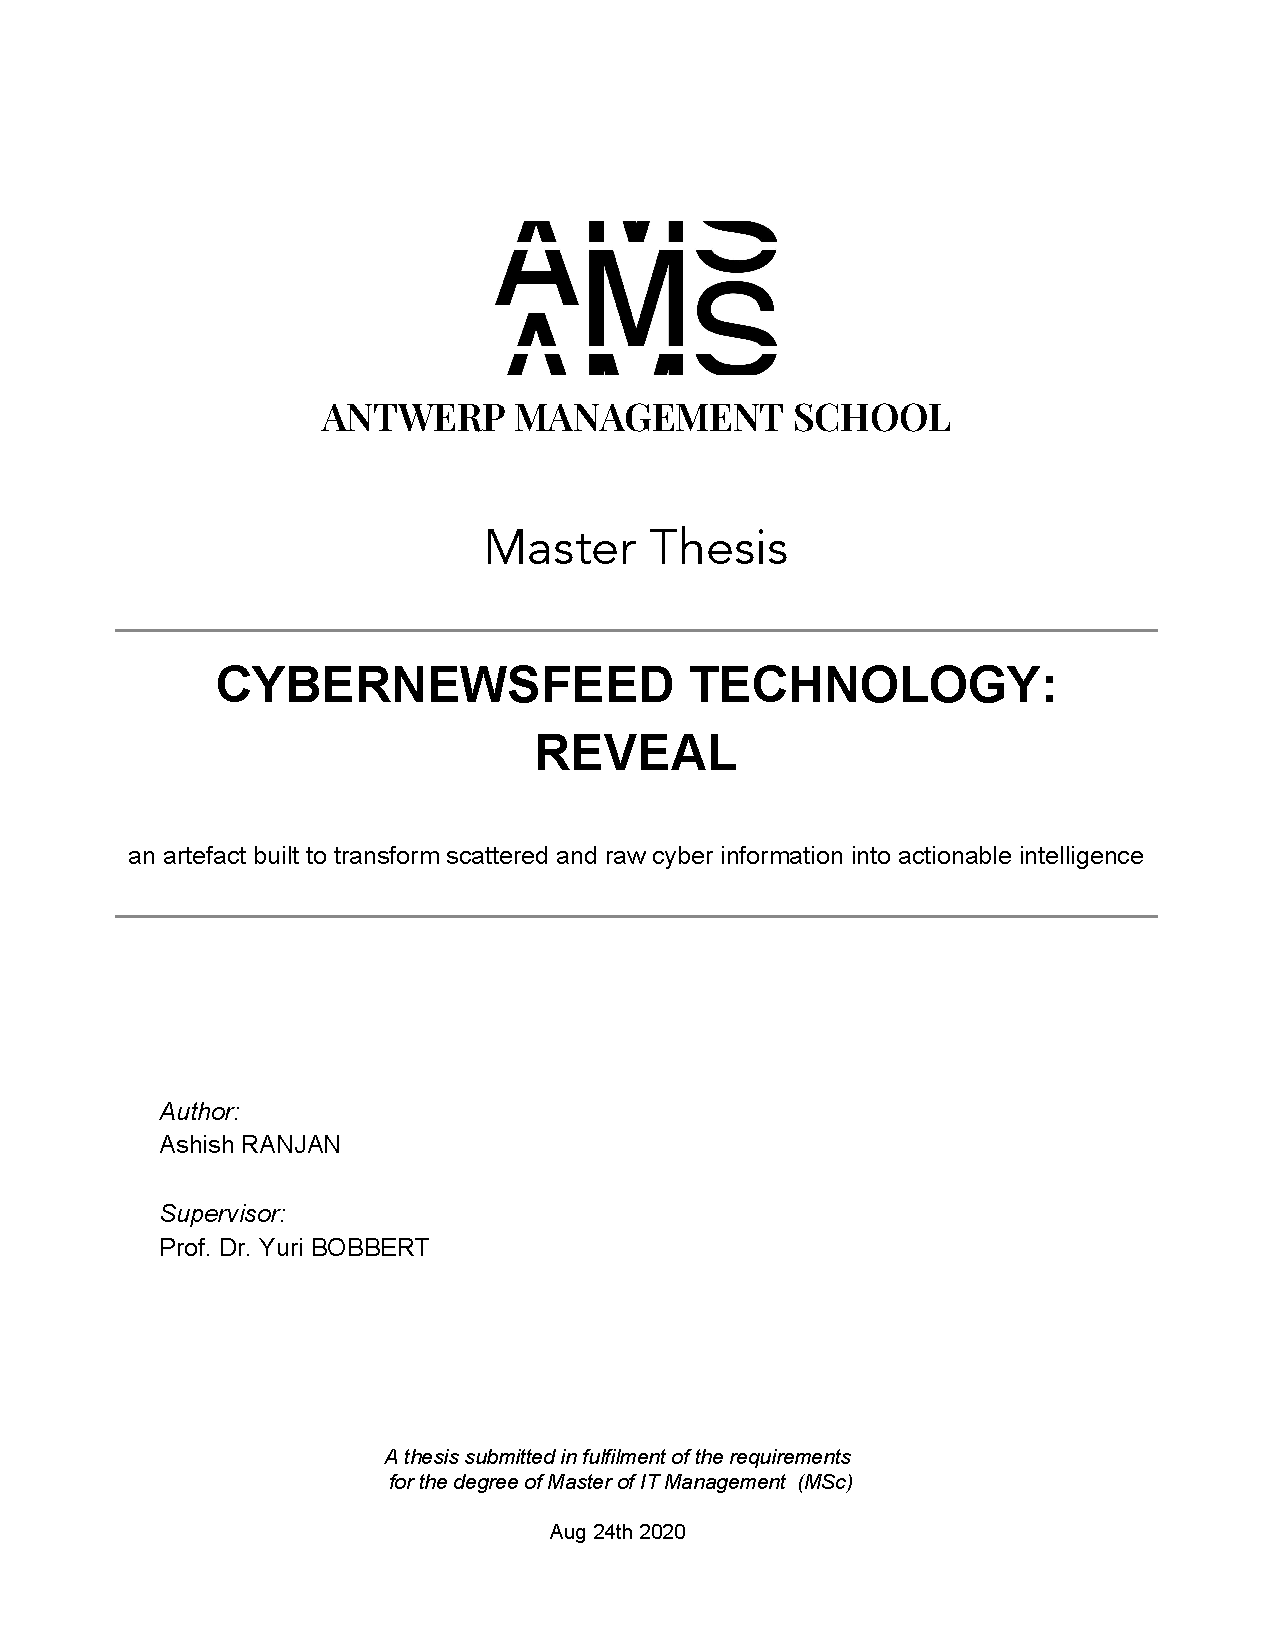
\includepdf[pages=-]{frontpage-ams.pdf}
%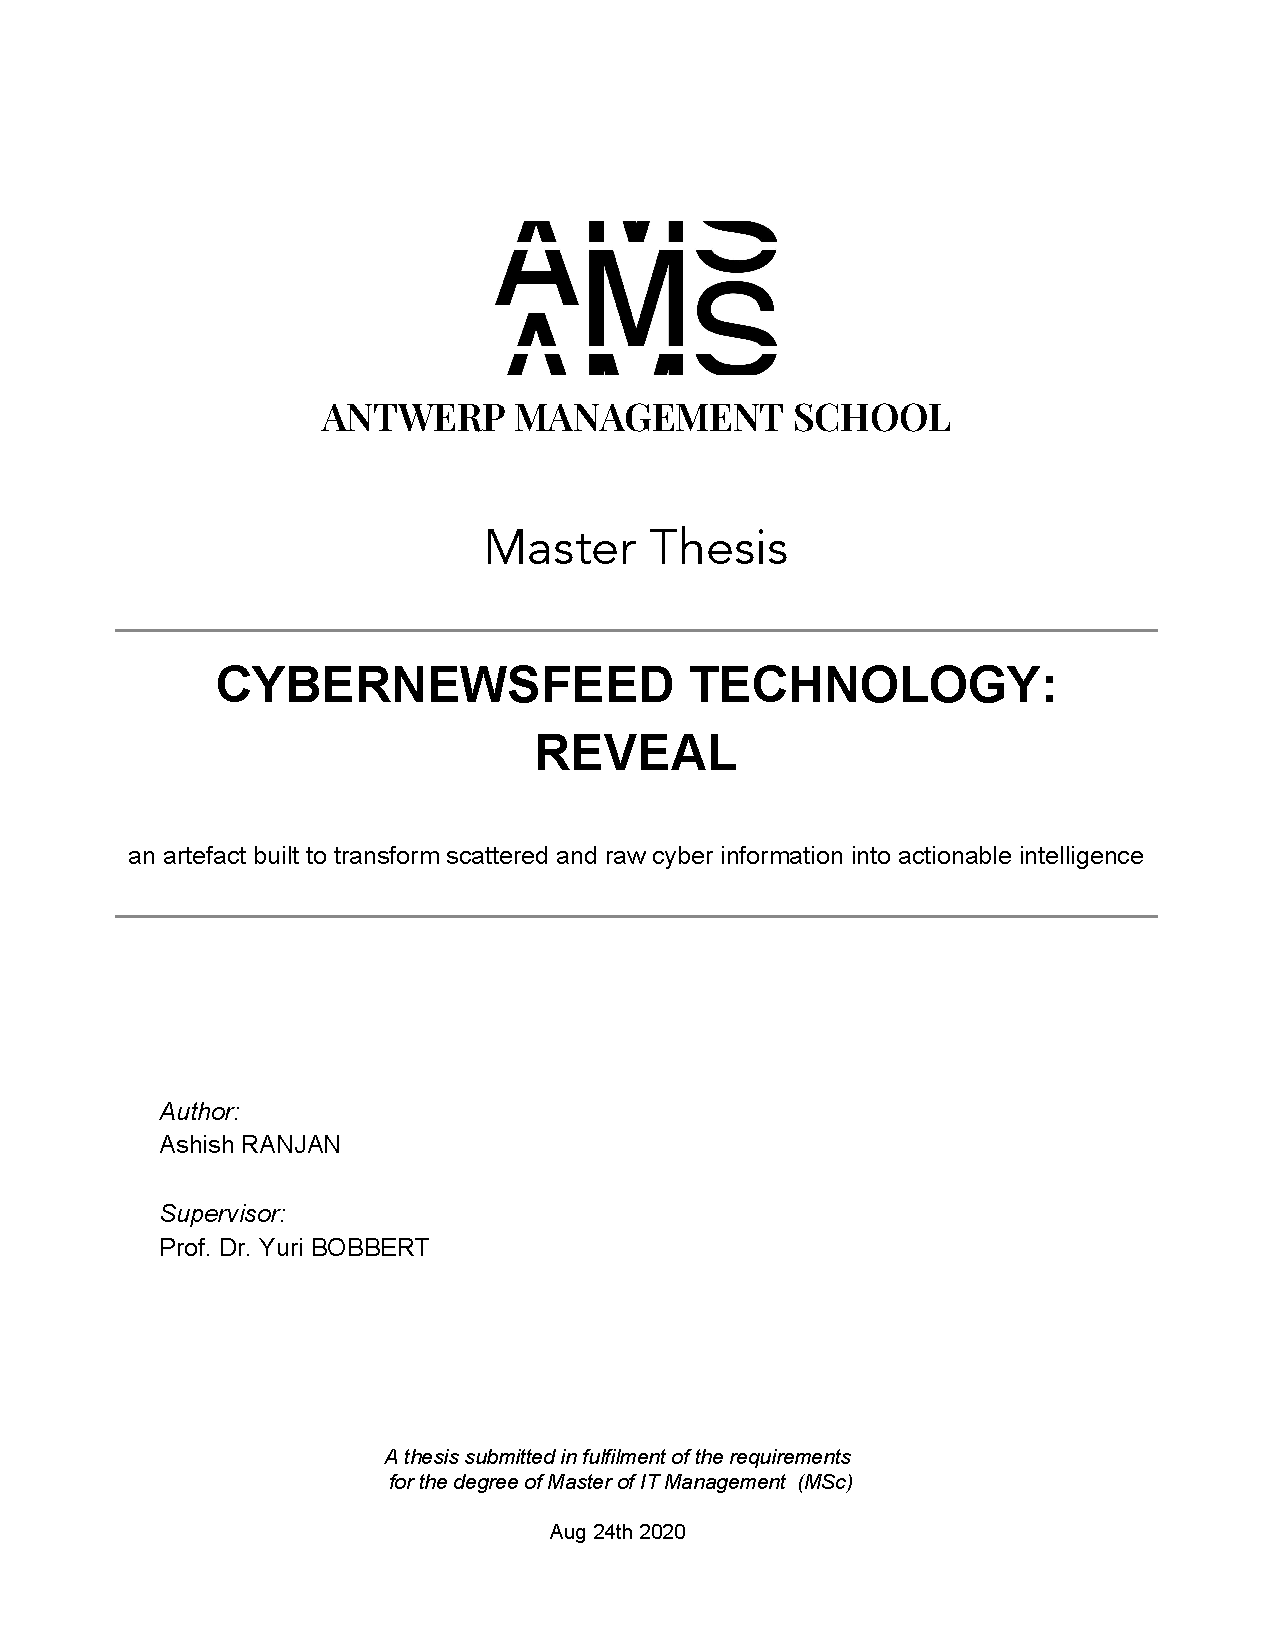
\includepdf{frontpage-ams.pdf}
\thispagestyle{empty}


\frontmatter % Use roman page numbering style (i, ii, iii, iv...) for the pre-content pages

\pagestyle{plain} % Default to the plain heading style until the thesis style is called for the body content

%----------------------------------------------------------------------------------------
%	TITLE PAGE
%----------------------------------------------------------------------------------------

% Chapter 2

\chapter{Executive Summary} % Main chapter title

\label{Chapter0_Executive Summary} % For referencing the chapter elsewhere, use \ref{Chapter1} 

%----------------------------------------------------------------------------------------



%----------------------------------------------------------------------------------------

%\section*{Introduction}

This Master thesis project aims to improve the quality of cyber intelligence by solving the volumetric problems of scattered cyber information over the internet by implementation of an artefact. 
An artefact prototype 
\enquote{Cybernewsfeed Technology: REVEAL} 
has been built by implementing Creative process 
\citep{mednick1962associative} under the Design Science Research (DSR) framework 
\citep{bobbert2017exploring}. 
This technology converts a \enquote{Scattered \& Raw} 
cyber information 
(FIGURE \ref{fig:cyber-feed-info}), 
into an \enquote{Actionable} Cyber Intelligence (FIGURE \ref{fig:cyber-feed-intel}). 
This artefact has been validated by a Focus Group in a Group Support Session (GSS)\citep{briggs2001thinklets}. 
Additionally, a feasibility check was done via a simulation. 
The outcome of the simulated system was validated positively by the Focus Group. 

%----------------------------------------------------------------------------------------

\begin{figure}[!htbp]
  \centering
  \subfloat["Scattered \& Raw" Cyber Information]{\fbox{\includegraphics[width=0.45\textwidth]{cyber-feed-info.PNG}\label{fig:cyber-feed-info}}}\hspace{1em}
  \subfloat["Actionable" Cyber Intelligence for CISO ]{\fbox{\includegraphics[width=0.45\textwidth]{cyber-feed-intel.PNG}\label{fig:cyber-feed-intel}}}
  \caption{"Scattered \& Raw" vs "Actionable" cyber newsfeed}
\end{figure}


The current status quo is that cyber news or cyber information are being pushed via multiple media \enquote{RSS, mail, WWW, news feeds etc} to multiple organisational stakeholders in a scattered way \citep{schales2011stream}
and are manually interpreted, 
this causes a dilute and incomplete picture 
\citep{liao2016acing}. 
Especially in a world where threats emerge in numbers and sophistication. In 2018 there were one billion unique malware samples counted \citep{kucuk2020deceiving}.
 
 
%\begin{figure}[ht]
%    \centering
%    \fbox{
\includegraphics[width=0.4\linewidth]{Figures/problem2.png}}
%    \caption{Problem with information from multiple feeds. }
%    \label{fig:problem2}
%\end{figure}



% \bigbreak

%----------------------------------------------------------------------------------------

\section*{The Solution: Cybernewsfeed Technology }

To deal with the volumetric cyber newsfeed information, the artefact \enquote{Cybernewsfeed Technology: REVEAL} was build. The design of the artefact is based on literature research on existing threat intelligence tools and users requirements from ON2IT.

The artefact is a software prototype and is created by applying Creative process
\citep{mednick1962associative}.
This artefact collects, processes and transforms cyber newsfeeds into actionable and organisation-specific valuable data. The data aids security professionals in making better decisions.

The artefact helps  organizations getting organisation-specific  actionable  cyber newsfeeds. 
%--------------------------------------

%We build an artefact to see, if we could overcome the volumetric problem. To design the artefact, a literature research was done on existing capability of the threat intelligence platforms and then, the requirements of an ideal system were explored with the cyber security experts. The gaps found between the existing threat intelligence system and the required system was addressed. A new artefact prototype \enquote{Cybernewsfeed Technology: REVEAL} was build and validated. 

\subsection*{Prototype requirement, design and validation}

The first iteration of the requirements for the artefact prototype was collected with the help of ON2IT team. If the reader wants to see the list of requirements, these requirements are are mentioned in TABLE  \ref{tab:requirement-appendix} of Appendix \ref{AppendixA}.

Based on the feedback of the Focus group, I concluded that It is very important to add context and meaning to the cyber information so that it transforms to a cyber intelligence (See FIGURE  \ref{fig:problem-context}).
 

%\subsubsection*{Requirement}\label{Requirement_ES}

%The artefact required some extra code and business logic to filter the relevant cyber newsfeed, some Graphical User Interface (GUI) to interact with cyber newsfeed data and some mechanism to adjust the configurable parameters. In addition to these requirements, the cyber newsfeed data sources needs to kept regularly sanitized.
%Some requiremens needed involvements of human intervention, for example, to perform detail analyis, to add advisory information, and to able to perform editorial checks before shipping to stakeholders. The above requirements would make the cyber newsfeed information not only intelligent but also actionable.

%\subsubsection*{Solution design}

%Based on the requirement mentioned in above section 
%(\nameref{Requirement_ES}), 
%I started exploring existing open source tools to find the capabilities mentioned in section 
%(\nameref{Requirement_ES}). 
%After assessment of 23 different open source tools based on the assessment parameters in mentioned table \ref{table:assessment}, 
%I selected one tool for further customisation and development. 
%The solution artefact is build on top of this open source tool\footnote{Tool used in this thesis for cyber newsfeed collection \url{https://freshrss.org/}} and is made of three modules. 
%These modules comprise of processes, 
%activities and tools at implementation level. 
%The demo of these modules have shown the capability to transform a scattered cyber raw information into an actionable cyber intelligence.

%
\begin{table}
    \caption{Assessment Parameters for tool selection}
    \label{table:assessment}
    \centering{}
   \resizebox{0.75\textwidth}{!}{
    \begin{tabular}{|>{\columncolor[HTML]{ECB4E8}}l|l|}
    \toprule
      \rowcolor[HTML]{BFCEED} 
    
    \textbf{Assessment Parameters} & \textbf{Focus}\\
    \midrule
    Distribution & Open Source\\
    Application Support Forum  Available? & Ease of trouble shoot\\
    Application Active Since years & Old and stable\\
    Application's Last Issue resolved date & Most recent is better\\
    Functional Features &	More is better\\
    Database and GUI & User Friendly\\
   \bottomrule
 
    \end{tabular}
}
\end{table}



%\begin{figure}[ht]
%    \centering
%    \fbox{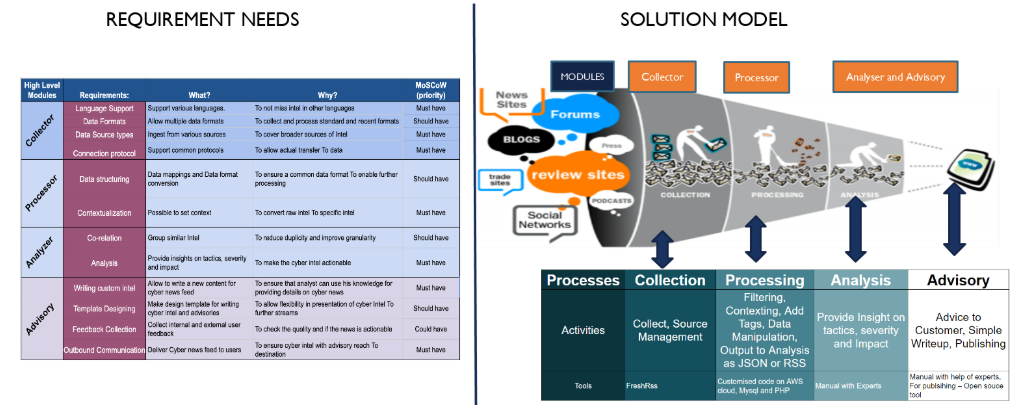
\includegraphics[width=1\linewidth]{Figures/requirement-solution.PNG}}
%    \caption{Requirement versus Solution design}
%    \label{fig:requirement-solution}
%\end{figure}

%\subsection*{Prototype Validation}

The created artefact was validated by the six members of the Focus Group and a CEO of a Cyber security company.

%\section*{Conclusion }



As confirmed by the Focus group participants, 
an  organization-specific cyber newsfeeds can be delivered to an organisation, by configuring the artefact. 
The output newsfeed from this artefact is complemented with the advisory of actionable steps based on the cyber newsfeed content
(see FIGURE \ref{fig:problem-context}).

\begin{figure}[ht]
    \centering
   \fbox{ 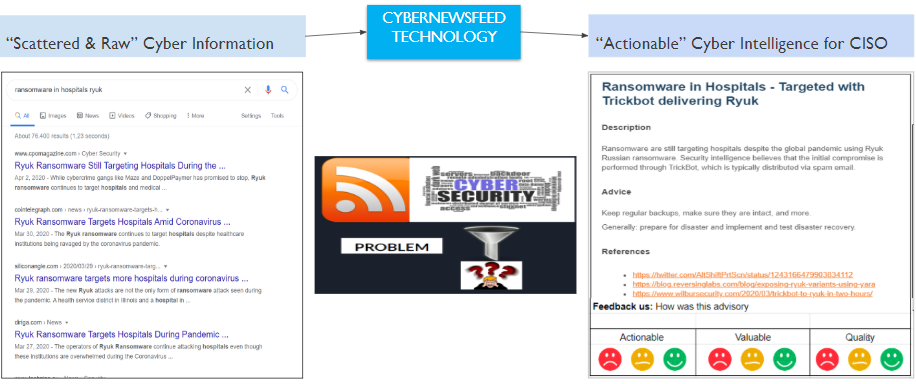
\includegraphics[width=1\linewidth]{Figures/problem-context.PNG}}
    \caption{Cybernewsfeed Technology attempt to address the issue}
    \label{fig:problem-context}
\end{figure}

The results of thesis has been rated useful both in term of its academic purpose and practical use by the stakeholders. The main highlight of this thesis is a demo video, depicting  the academic and rigor concepts being implemented.









\begin{titlepage}
\begin{center}

\vspace*{.06\textheight}
{\scshape\LARGE \univname\par}\vspace{1.5cm} % University name
\textsc{\Large Master Thesis}\\[0.5cm] % Thesis type

\HRule \\[0.4cm] % Horizontal line
{\huge \bfseries \ttitle\par}\vspace{0.4cm} % Thesis title
\HRule \\[1.5cm] % Horizontal line
 
\begin{minipage}[t]{0.4\textwidth}
\begin{flushleft} \large
\emph{Author:}\\
\href{https://www.linkedin.com/in/ashish-ranjan-30510115/}{\authorname} % Author name - remove the \href bracket to remove the link
\end{flushleft}
\end{minipage}
\begin{minipage}[t]{0.4\textwidth}
\begin{flushright} \large
\emph{Supervisor:} \\
\href{https://www.linkedin.com/in/yuribobbert/}{\supname} % Supervisor name - remove the \href bracket to remove the link  
\end{flushright}
\end{minipage}\\[3cm]
 

\includegraphics[width=50mm,scale=0.5]{Logo} 

\large \textit{A thesis submitted in fulfillment of the requirements\\ for the degree of \degreename}\\[0.3cm] % University requirement text
\textit{in the}\\[0.4cm]
\groupname\\\deptname\\[2cm] % Research group name and department name
 
%\vfill
{\large \today}\\[4cm] % Date
%{\usvardate\today}\\[0.4cm] % Date


%
\includegraphics{Logo} % University/department logo - uncomment to place it
 
\vfill
\end{center}
\end{titlepage}

%----------------------------------------------------------------------------------------
%	DECLARATION PAGE
%----------------------------------------------------------------------------------------

\begin{declaration}
\addchaptertocentry{\authorshipname} % Add the declaration to the table of contents
\noindent I, \authorname, declare that this thesis titled, \enquote{\ttitle} and the work presented in it are my own. I confirm that:

\begin{itemize} 
\item This work was done wholly or mainly while in candidature for a research degree at this University.
\item Where any part of this thesis has previously been submitted for a degree or any other qualification at this University or any other institution, this has been clearly stated.
\item Where I have consulted the published work of others, this is always clearly attributed.
\item Where I have quoted from the work of others, the source is always given. With the exception of such quotations, this thesis is entirely my own work.
\item I have acknowledged all main sources of help.
\item Where the thesis is based on work done by myself jointly with others, I have made clear exactly what was done by others and what I have contributed myself.\\
\end{itemize}
 
\noindent Signed:\\
\rule[0.5em]{25em}{0.5pt} % This prints a line for the signature
 
\noindent Date:\\
\rule[0.5em]{25em}{0.5pt} % This prints a line to write the date
\end{declaration}

\cleardoublepage

%----------------------------------------------------------------------------------------
%	QUOTATION PAGE
%----------------------------------------------------------------------------------------

\vspace*{0.2\textheight}

\noindent\enquote{\itshape 
Thanks to my solid mental strength, 
I would be finishing my Master's, 
during the period of Covid-Cobit. 
I had no earnings still all responsibilities, 
and I really enjoyed this time}\bigbreak

\hfill Ashish Ranjan

%----------------------------------------------------------------------------------------
%	ABSTRACT PAGE
%----------------------------------------------------------------------------------------

%\begin{abstract}
%\addchaptertocentry{\abstractname} % Add the abstract to the table of contents
%\textit{This study is an attempt to contribute to improve transformation process of cyber intelligence. 
%This piece of work examined the use of pre-configured parameters to filter
%the relevant and actionable cyber information from the internet sources (RSS feeds). 
%For that an exploration on existing tools were done and additional system was build on the top of one of the tools.  
% This contextualised cyber information is further enhanced by the cyber analysts and editors to make it actionable and intelligent cyber news feed.
%With the use of this technology, the role of cyber analysts are also very important to transform a raw cyber newsfeed information into cyber intelligence. According to the research conclusion, there is a need of such a technology, where the stakeholders wants to receive the organisation-specific news immediately as a text messages and are willing to invest a descent amount.}
%
%\end{abstract}

%----------------------------------------------------------------------------------------
%	ACKNOWLEDGEMENTS
%----------------------------------------------------------------------------------------
%\input{./Chapters/Chapter0_acknowledgment}

%----------------------------------------------------------------------------------------
%	ACKNOWLEDGEMENTS
%----------------------------------------------------------------------------------------
\begin{acknowledgements}
This master's journey changed my life, my knowledge improved, I feel mature and stronger.
\bigbreak
Although I am the one writing this thesis to finalise but the journey to the finish line would have never been possible without the blessings, wishes and hopes of the people whom I mentioned here.
\bigbreak
First acknowledgment to my Father Arvind Kumar Singh, my Mother Saraswati Singh, my brother in law Nidish and to my wife Pooja who suggested to take this course.
\bigbreak
Second, to my line managers Sameer Sheety and Hans Vancompernolle who supported me with the decision. I am very thankful for their continuous support during the course program.
\bigbreak
Then to the participants of the Focus Group for the validation session.
1) Barry Derksen
2) Joshua Paffen
3) Marcel de Haan
4) Mark Butterhoff
5) Nico Kuijper
6) Rion Rijker 
7) Pascale van Damme

\bigbreak
At the Antwerp Management School side, my sincere thanks to Stevan de Haes and Danny Lauwerns for considering my application and allowing to pursue this course. Their help and flexibility is beyond the scope of my write up.
\bigbreak
And now to my friends at AMS, I made a good reputation and connection with almost every one, but I must mention the special one here because of their support to me in one or another way. Theo, Jan, Dave, Titi, Gafoor, Tapan, Jousua, Amie, Nick, Laurence, Stefan, Jeroen, Benoit, Tim, Dorian, Chao, Maria, Joris, Pascale, Ahemad and the list is never ending. I am really lucky to have a very nice group of people in 2018-2020 batch. Edzo is the one who supported me at almost every part of my research and finalising this thesis.
\bigbreak
I am also grateful to ON2IT Research and Development department(Jean-Hugues Migeon and Jeroen Scheerder) for helping me understand the domain quickly,  my three proof readers Edzo Botjes, Hatem Smine and Tapan Kumar who helped reviewing this work.
\bigbreak
Finally, a very special thanks to Yuri Bobbert Sir for his belief in my potential. Thanks to his direction, his time and effort investments in me, it was a real boom, and I know he is the real "Guru", my project advisor\ldots


\end{acknowledgements}

%----------------------------------------------------------------------------------------
%%----------------------------------------------------------------------------------------
%	ACKNOWLEDGEMENTS
%----------------------------------------------------------------------------------------
\begin{acknowledgements}
This master's journey changed my life, my knowledge improved, I feel mature and stronger.
\bigbreak
Although I am the one writing this thesis to finalise but the journey to the finish line would have never been possible without the blessings, wishes and hopes of the people whom I mentioned here.
\bigbreak
First acknowledgment to my Father Arvind Kumar Singh, my Mother Saraswati Singh, my brother in law Nidish and to my wife Pooja who suggested to take this course.
\bigbreak
Second, to my line managers Sameer Sheety and Hans Vancompernolle who supported me with the decision. I am very thankful for their continuous support during the course program.
\bigbreak
Then to the participants of the Focus Group for the validation session.
1) Barry Derksen
2) Joshua Paffen
3) Marcel de Haan
4) Mark Butterhoff
5) Nico Kuijper
6) Rion Rijker 
7) Pascale van Damme

\bigbreak
At the Antwerp Management School side, my sincere thanks to Stevan de Haes and Danny Lauwerns for considering my application and allowing to pursue this course. Their help and flexibility is beyond the scope of my write up.
\bigbreak
And now to my friends at AMS, I made a good reputation and connection with almost every one, but I must mention the special one here because of their support to me in one or another way. Theo, Jan, Dave, Titi, Gafoor, Tapan, Jousua, Amie, Nick, Laurence, Stefan, Jeroen, Benoit, Tim, Dorian, Chao, Maria, Joris, Pascale, Ahemad and the list is never ending. I am really lucky to have a very nice group of people in 2018-2020 batch. Edzo is the one who supported me at almost every part of my research and finalising this thesis.
\bigbreak
I am also grateful to ON2IT Research and Development department(Jean-Hugues Migeon and Jeroen Scheerder) for helping me understand the domain quickly,  my three proof readers Edzo Botjes, Hatem Smine and Tapan Kumar who helped reviewing this work.
\bigbreak
Finally, a very special thanks to Yuri Bobbert Sir for his belief in my potential. Thanks to his direction, his time and effort investments in me, it was a real boom, and I know he is the real "Guru", my project advisor\ldots


\end{acknowledgements}

%----------------------------------------------------------------------------------------

%----------------------------------------------------------------------------------------
%	LIST OF CONTENTS/FIGURES/TABLES PAGES
%----------------------------------------------------------------------------------------

\tableofcontents % Prints the main table of contents

\listoffigures % Prints the list of figures

\listoftables % Prints the list of tables

%----------------------------------------------------------------------------------------
%	ABBREVIATIONS
%----------------------------------------------------------------------------------------

\begin{abbreviations}{ll} % Include a list of abbreviations (a table of two columns)

%\textbf{LAH} & \textbf{L}ist \textbf{A}bbreviations \textbf{H}ere\\
% \textbf{WSF} & \textbf{W}hat (it) \textbf{S}tands \textbf{F}or\\


\textbf{API} &
\textbf{A}pplication \textbf{P}rogramming \textbf{I}nterfaces\\
\textbf{BIS} &
\textbf{B}usiness \textbf{I}nformation \textbf{S}ecurity\\
\textbf{CERT} &
\textbf{C}omputer \textbf{E}mergency \textbf{R}esponse \textbf{T}eam\\
\textbf{CISO} &
The \textbf{C}hief \textbf{I}nformation \textbf{S}ecurity \textbf{O}fficer\\
\textbf{COVID} &
\textbf{Co}rona \textbf{Vi}rus \textbf{d}isease\\
\textbf{CSIRT} &
A \textbf{c}omputer \textbf{s}ecurity \textbf{i}ncident \textbf{r}esponse \textbf{t}eam\\
\textbf{CVE} &
\textbf{C}ommon \textbf{V}ulnerabilities and \textbf{E}xposures\\
\textbf{DSR} &
\textbf{D}esign \textbf{S}cience \textbf{R}esearch\\
\textbf{FBI} &
\textbf{F}ederal \textbf{B}ureau of \textbf{I}nvestigation division\\
\textbf{GSS} &
\textbf{G}roup \textbf{S}upport \textbf{S}ystem\\
\textbf{IDF} &
\textbf{I}nverse \textbf{D}ocument \textbf{F}requency\\
\textbf{IOC} &
\textbf{I}ndicator \textbf{o}f \textbf{C}ompromise\\
\textbf{NCSC} &
The \textbf{N}ational \textbf{C}yber \textbf{S}ecurity \textbf{C}entre\\
\textbf{NIST} &
The \textbf{N}ational \textbf{I}nstitute of \textbf{S}tandards and \textbf{T}echnology\\
\textbf{NVD} &
\textbf{N}ational \textbf{V}ulnerability \textbf{D}atabase\\
\textbf{OEM} &
\textbf{O}riginal \textbf{E}quipment \textbf{M}anufacturer\\
\textbf{RSS} &
\textbf{R}DF \textbf{S}ite \textbf{S}ummary or \textbf{R}eally \textbf{S}imple \textbf{S}yndication\\
\textbf{SANS} &
\textbf{S}ysAdmin, \textbf{A}udit, \textbf{N}etwork, and \textbf{S}ecurity\\
\textbf{SIEM} &
\textbf{S}ecurity \textbf{I}nformation and \textbf{E}vent \textbf{M}anagement\\
\textbf{SOC} &
\textbf{S}ecurity \textbf{O}perations \textbf{C}enter\\
\textbf{STIX} &
\textbf{S}tructured \textbf{T}hreat \textbf{I}nformation e\textbf{X}pression\\
\textbf{TF} &
\textbf{T}erm \textbf{F}requency\\
\textbf{TI} &
\textbf{T}hreat \textbf{I}ntelligence\\
\textbf{TIP} &
\textbf{T}hreat \textbf{I}ntelligence \textbf{P}latform\\
\textbf{TTPs} &
\textbf{T}actics, \textbf{T}echniques and \textbf{P}rocedures\\
\textbf{URL} &
\textbf{U}niform \textbf{R}esource \textbf{L}ocator\\
\textbf{WWW} &
\textbf{W}orld \textbf{W}ide \textbf{W}eb\\
\textbf{US-CERT} &
The \textbf{U}nited \textbf{S}tates \textbf{C}omputer \textbf{E}mergency \textbf{R}eadiness \textbf{T}eam\\
\textbf{USB} &
\textbf{U}niversal \textbf{S}erial \textbf{B}us\\
\textbf{VSM} &
The \textbf{V}ector-\textbf{S}pace \textbf{M}odel\\
\textbf{PINA} &
 \textbf{P}ublic-\textbf{I}nfo \textbf{N}ot \textbf{A}vailable\\
\textbf{NOC} &
 \textbf{N}etwork \textbf{O}peration \textbf{C}enter \\
\textbf{ROI} &
 \textbf{R}eturn \textbf{o}n \textbf{I}nvestment \\


\end{abbreviations}

%----------------------------------------------------------------------------------------
%	PHYSICAL CONSTANTS/OTHER DEFINITIONS
%----------------------------------------------------------------------------------------

%\begin{constants}{lr@{${}={}$}l} % The list of physical constants is a three column table

% The \SI{}{} command is provided by the siunitx package, see its documentation for instructions on how to use it

%Speed of Light & $c_{0}$ & \SI{2.99792458e8}{\meter\per\second} (exact)\\


%Constant Name & $Symbol$ & $Constant Value$ with units\\

%\end{constants}

%----------------------------------------------------------------------------------------
%	SYMBOLS
%----------------------------------------------------------------------------------------

\begin{symbols}{lll} % Include a list of Symbols (a three column table)

%$a_1$ & distance & \si{\meter} \\
%$P$ & power & \si{\watt} (\si{\joule\per\second}) \\
%Symbol & Name & Unit \\
$p_1$ & source quality metrics  & extensive parameter1\\
$i$ & sequence & number\\
$\max y_i$ & maximum & number\\
$o_i$ & sum & sum of filled-in optional properties\\
$z$ & total & number\\
$\sum\limits_{n=1}^{z}$ & limit & integration(1 to z)\\
 
\addlinespace % Gap to separate the Roman symbols from the Greek

%$\omega$ & angular frequency & \si{\radian} \\




\end{symbols}

%----------------------------------------------------------------------------------------
%	DEDICATION
%----------------------------------------------------------------------------------------

\dedicatory{Dedicated to my kids Aahaan and Aarna, they ofen used to come and ask me, If I could spend some time with them. 
\bigbreak And I know the time I have invested in this thesis, It was their time\ldots} 

%----------------------------------------------------------------------------------------
%	THESIS CONTENT - CHAPTERS
%----------------------------------------------------------------------------------------

\mainmatter % Begin numeric (1,2,3...) page numbering

\pagestyle{thesis} % Return the page headers back to the "thesis" style

% Include the chapters of the thesis as separate files from the Chapters folder
% Uncomment the lines as you write the chapters


\include{Chapters/Chapter2} 
% Chapter 3

\chapter{Key Concepts and Terms About Cyber newsfeed} % Main chapter title

\label{Chapter3key_concepts-and-terms} % For referencing the chapter elsewhere, use \ref{Chapter3} 

%----------------------------------------------------------------------------------------



%----------------------------------------------------------------------------------------

\section{Introduction} 
This chapter provides key concepts, 
keywords and important terms which are both 
1) about the cyber newsfeeds and 
2) are related to cyber newsfeeds.
I have used the mindmap approach \citep{buzan2006mind}  
to list the central concepts first 
and then map the required concepts 
in relation to each other\footnote{Refer to Appendix \ref{AppendixChapter3} for more details}. 
Understanding the concepts mentioned in the mindmap 
are required to understand the problem context 
and the subsequent chapters of this master thesis. 
The terms and the concepts introduced in this chapter 
are relevant throughout the rest of this master thesis. I have made use of tools, technology, prototype and artefact for \enquote{Cybernewsfeed Technology: REVEAL} and they denotes the same thing.



%----------------------------------------------------------------------------------------
\section{Cyber Threat - Information vs. Intelligence and link to newsfeed}
It is critically important to acknowledge  
the fundamental difference between 
raw information and processed information in context of cyber security. 
The processed information becomes intelligence 
if it is evaluated to be useful for the stakeholders \citep{liew2013dikiw}. 
A useful comparison of the difference between information and intelligence is summarized below in 
TABLE \ref{table:info-intel} \citep{threat-intelligence}.
The cyber newsfeed is a raw information, and it is important to highlight that the processing of a cyber newsfeeds makes cyber intelligence.
%----------------------------------------------------------------------------------------


\begin{table}[htbp!]
   \setlength{\arrayrulewidth}{0.1mm}
    \setlength{\tabcolsep}{3pt}
    \renewcommand{\arraystretch}{1.0}

    \centering{}
 
    \caption{Difference: Information vs Intelligence}
    \label{table:info-intel}
    
    \begin{tabularx}{0.9\linewidth}{| X|X|} 
    
%    |a|>{\columncolor[HTML]{FFFFFF}}C|C|C|
     \arrayrulecolor[HTML]{06000A}
        %% Table Body
        \hline
       
         \rowcolor[HTML]{BFCEED} INFORMATION & INTELLIGENCE \\
        \hline
      Raw, unfiltered data	&	Processed, sorted, and distilled information	\\
      \hline
Unevaluated when delivered	&	Evaluated and interpreted by trained expert analysts	\\
\hline
Aggregated from virtually every source	&	Aggregated from reliable sources and cross correlated for accuracy	\\
\hline
May be true, false, misleading, incomplete, relevant, or irrelevant	&	Accurate, timely, complete (as possible), assessed for relevancy	\\
       
        \hline
    \end{tabularx}

\end{table}

\FloatBarrier



\section{The word \enquote{cyber newsfeed}}
During my interaction with a group of cyber professionals working at 
ON2IT\footnote{A cybersecurity company \url{https://www.linkedin.com/company/on2it-b-v-/}} (Jean-Hugues Migeon, Jeroen Scheerder, Richard Stone, Harald van Wijner and Brandon Brown), I heard it first time but could not find a direct mention  in academic literatures. 
Let’s start by looking into the meaning of the word  \textit{cyber newsfeed}. 
%The term \textit{cyber newsfeed} as a word does not exist in the literature. 
It's a composite of three words: 
1) \textit{cyber}
2) \textit{news} and 
3) \textit{feed} altogether for ease and as a common jargon among cyber securities practitioners. Essentially cyber newsfeeds are Really Simple Syndication (RSS)\footnote{RSS \url{https://en.wikipedia.org/wiki/RSS}} feeds published at various websites and the term is used as common jargon among cyber security practitioners. 


\section{What is cyber newsfeed?}

In this master thesis a cyber newsfeed is a news information\footnote{Look at FIGURE \ref{fig:darkreading} and in FIGURE \ref{fig:databreaches} in Appendix \ref{AppendixChapter3}}  
or news items which are specific to the cybersecurity world 
and is available on the internet \footnote{Cyber newsfeed websites at 1) \url{https://www.databreaches.net } and 2) \url{ https://www.darkreading.com}}. 
So far as explored on Internet, the available cyber newsfeed items were also found as audio and text. 
It would be nice to explain it in more detail by citing one example from a website providing cyber newsfeed. 
For example, (see FIGURE \ref{fig:cyber-feed}). In the example, the four cyber related news items are listed from a website publishing cyber newsfeeds. 

\begin{figure}[htbp!]
\centering
    \fbox{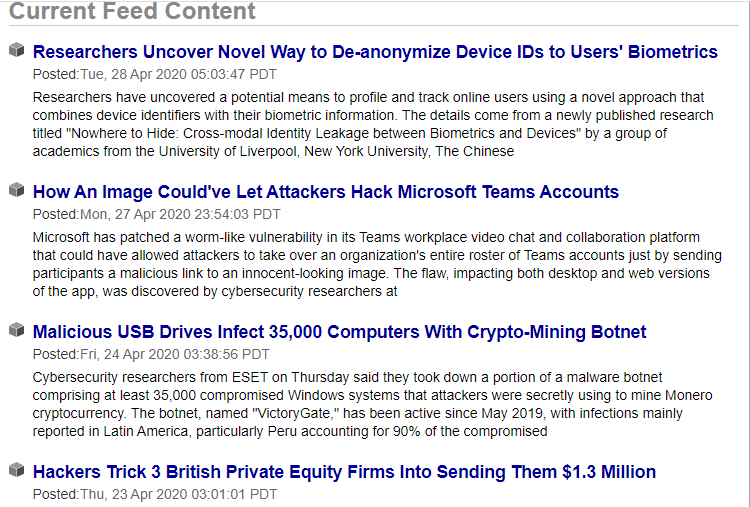
\includegraphics[scale=0.45]{Figures/cyber-feed}}
    \caption{Raw Cyber newsfeed from source \citep{news-feed}}
    \label{fig:cyber-feed}
\end{figure}
\FloatBarrier

Here, we see how a cyber newsfeed reading pane normally looks. 
It is a list of  cyber newsfeed items presented at a cyber news publishing  website \citep{news-feed}. 
The general construct of a cyber newsfeed item is 
1) one liner headline 
2) date and time of the cyber news posted and 
3) a more detailed paragraph about that particular news shown under the headline. 

The actual content of the detailed newsfeed item could be more, may be it is hosted with some pictures or links explaining some cyber issues and more detail on the particular cyber newsfeed item. Let see the other informations available in a cyber newsfeed item with an example from \citep{news-feed}.

For instance, the cyber news about \enquote{Malicious USB Drives…}, as shown in FIGURE \ref{fig:cyber-feed}, when accessed at \citep{news-feed} on the web-page gave more information about the cyber newsfeed item.  The extra information retrieved on the news item are the following: 

\begin{itemize}
  \item \textbf{Author} of this cyber newsfeed item.
  \item \textbf{Place of origin} of this cyber newsfeed item.
  \item \textbf{Impacted}  users, machines and servers.
  \item Potential \textbf{loss} due to Malicious USB Drives.
  \item \textbf{Mitigation} ways to avoid this.
\end{itemize}

The goal of a cyber newsfeed is to provide enough information about the cyber news topic at the time of the publication at the website. 
It is also good to know that publications of such cyber newsfeed items do not follow a common standard and the structure of the contents published vary from one website to another website. This was confirmed after comparing the contents of two websites\footnote{Look at Appendix \ref{AppendixChapter3} for the difference between \url{https://www.databreaches.net}
(figure \ref{fig:databreaches}) 
and content of 
\url{https://www.darkreading.com.} 
(figure \ref{fig:darkreading})} 
1) \url{https://www.databreaches.net} and 
2) \url{ https://www.darkreading.com}.

\section{Why do we need cyber newsfeed?}

The objectives of the cyber newsfeeds are to provide timely cyber awareness and information about  any ongoing cyber threats. With such informations, the organizations can prepare themselves to avoid or mitigate certain cyber risks which may impact business operations \citep{ring2014threat}. 
Such cyber informations acknowledged by the organisation  will ensure that the organization’s critical business information is safe from the vulnerabilities related to similar threats.
It helps organizations to understand the motivation of a threat actor\footnote{\url{https://en.wikipedia.org/wiki/Threat_actor}}, 
their behaviour and technique of attack \citep{jouini2014classification}. 
It also helps to identify the vulnerable system and the input points of attack. 
The designated and responsible cyber security team can use this information as a heads up and start analysing their situation and get prepare in case of a potential attack \citep{chismon2015threat}. 

Some examples of such information extracted from a cyber newsfeed items which may be useful for the awareness of security professionals, are as listed below:
\begin{itemize}
    \item \textbf{Indicators of Compromise (IOCs):} 
    System artefacts or observable that contain patterns, 
    such as malicious Internet Protocol addresses (IPs) or hashes of files containing malware, 
    which can help identify suspicious or malicious activity \citep{hyeisuncyber}.
    
    \item \textbf{Tactics, Techniques and Procedures (TTPs): }
    Description of the behaviour of an actor that can assist operational activities, such as details of exploits and malware delivery mechanisms. TTPs include tradecrafts, i.e., behaviour used to conduct a malicious activity, infrastructure used to deliver malicious content or maintain command and control capabilities, and attackers’ intentions 
    \citep{shahi2018tactics}. 
    
    \item \textbf{Security alerts:} 
    Notification, usually human-readable regarding security issues, such as vulnerabilities 
    \citep[page 189]{RFC2828}. 
    
    \item \textbf{Threat intelligence reports:} 
    Collections of threat intelligence for various topics, such as threat actors, malware and attack techniques 
    \citep{ring2014threat}. 
   
    
    \item \textbf{Vulnerabilities:} 
    Known weaknesses in software implementations or procedures, and corresponding mitigations, such as security patches. Although in the information security literature, vulnerabilities are not threats, they are considered as an important component in the cyber threat information sharing ecosystem 
    \citep{rantos2020interoperability}. 
    
\end{itemize}

\subsection{Practical usage in Security Operations Center
(SOC) department }

The security operations centre of any organization using Information Technology systems protects Information and Information systems, by performing tasks, like cyber Intel collection, analysis, distribution, creation and fusion
\citep{onwubiko2015cyber}. 
These cyber newsfeeds are also used in threat assessment and to establish new trend on old cyber newsfeeds items 
\citep{zimmerman2014ten}.

\subsection{Where does it fit into big picture?}

Since the cyber newsfeed items is a information and is related to Cyber, 
we can say that cyber newsfeed item is a kind of cyber information. 
I would say they are fuel to cyber threat
\citep[page 169]{RFC2828} Intelligence Sharing Platforms.  
In FIGURE \ref{fig:TIP-model}, 
the data as cyber newsfeed is being collected from various sources and 
is getting processed for a more actionable information transformation.

\begin{figure}
\centering
    \fbox{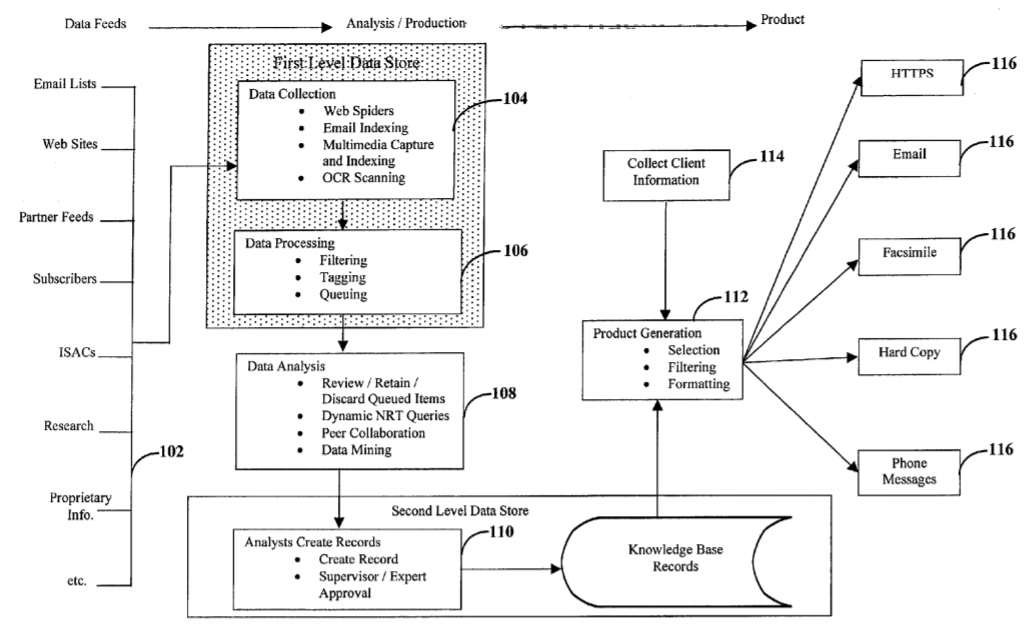
\includegraphics[scale=.63]{Figures/TIP-model.png}}
    \caption{System and Method of data collection, Processing, Analysis, and annotating Cyber threats \citep{edwards2002system}}
    \label{fig:TIP-model}
\end{figure}

\section{How are cyber newsfeeds made? Who are the producers?}

Cyber newfeed creation is a work of cyber security professionals working individually or for the organizations. 
These security professionals are the one, 
who focus on one or more security domains or practice and also keep learning from the hackers community 
\citep{mahmood2010moving}. 
They, then collaborate and share their respective findings about a certain threat or group of threats openly; 
among themselves, 
and on the internet as an information
or an intelligence for the awareness among security defenders. 
The focus area of such information may vary from vulnerabilities,
incident response, identifying intrusions, 
data breaches and potential threats 
\citep{rantos2020interoperability}. 
Vendors providing hardware and software products, 
manufactures of IT hardware and 
software products are also the major contributors of cyber newsfeed. 
For example, Microsoft releases information about its patches on its website\footnote{Microsft patches updates: \url{https://portal.msrc.microsoft.com/en-us/security-guidance.}}.

\section{How are cyber newsfeeds consumed? Who are the consumers?}

The collection and processing of cyber newsfeed  
depends on the purpose of cyber newsfeeds items. 
If the sole purpose is just reading then, 
an individual can explore the website producing cyber newsfeeds items 
his particular interests area.  
I want to highlight that, 
an automated collection system can also be configured 
to collect cyber newsfeed items from different sources and 
store in a single database 
\citep{sauerwein2017threat}. 
Another case is where specialized cyber security companies scan 
the web for all known and trusted cyber newsfeed and 
collect via dedicated servers into their own cyber Intelligence system 
to run analytics and make it selective and relevant. 
Like ON2IT has its own setup for collecting cyber newsfeed items. 
Cyber newsfeed consumers vary from people to organization, 
people may include security analysts, security officers, 
security advisors, security architects and general IT users 
\citep{shackleford2015s}.

\section{What are the sources of cyber newsfeeds?}

There is no “standard” list of 
cyber newsfeed or cyber information sources, 
however there are huge numbers of sources that are free and 
are open to access the cyber newsfeeds items. 
For illustration, 
here is a list of links that I have found as a good example on internet. 
The sources were working perfectly at the time of writing (Aug 2020) this thesis.
it is possible that some of the websites 
may not work at later point of time, 
but it is easy to find alternative websites containing similar information. 
The examples of the cyber newsfeed sources 
are based on different type of cyber newsfeed 
or information contents.

\begin{itemize}
    \item \textbf{General technology and security trends:} 
        \begin{itemize}
            \item Schneier on Security Blog: 
            \url{http://www.schneier.com} 
            
            \item Krebs on Security: 
            \url{http://krebsonsecurity.com}
            
            \item Security Dark Reading: 
            \url{http://www.darkreading.com}
            
            \item Slashdot: 
            \url{http://slashdot.org}
            
            \item Securosis: 
            \url{https://securosis.com/blog}
            
        \end{itemize}

    \item \textbf{Threat intelligence }
        \begin{itemize}
            \item Team Cymru (also has subscription service): 
            \url{http://www.team-cymru.org}
            
            \item FBI cybercrime information: 
            \url{http://www.fbi.gov/about-us/investigate/cyber/cyber}
            
        \end{itemize}
        
    \item \textbf{Malware and threats }
        \begin{itemize}
            \item SANS Internet Storm Center: 
            \url{http://isc.sans.edu}
            
            \item Dshield: 
            \url{http://www.dshield.org}
            
            \item Offensive Security’s Exploit Database: \url{http://www.exploit-db.com} 
            
        \end{itemize}
    
    \item \textbf{Bad domains, IP addresses, and other indicators} 
        \begin{itemize}
            \item Malware Domain List: 
            \url{http://www.malwaredomainlist.com}
            
            \item Unspam Technologies Project Honeypot: 
            \url{http://www.projecthoneypot.org/index.php}
            
            \item Shadowserver Foundation: 
            \url {http://www.shadowserver.org/wiki} 
            
        \end{itemize}
        
    \item \textbf{Automatic threat analyzers }
        \begin{itemize}
            \item Virustotal: 
            \url{http://www.virustotal.com}
            
            \item Metascan online: 
            \url{http://www.metascan-online.com}
            
        \end{itemize}
        
    \item \textbf{Patches and vulnerabilities} 
            \begin{itemize}
            \item MITRE’s\footnote{\url{https://en.wikipedia.org/wiki/Mitre_Corporation}} CVE: 
            \url{https://cve.mitre.org}
            
            \item NIST’s\footnote{\url{https://en.wikipedia.org/wiki/National_Institute_of_Standards_and_Technology}} National Vulnerability Database: 
            \url{http://nvd.nist.gov}
        \end{itemize}
        
\end{itemize}

Apart from these sources, 
some social networking sites like Twitter\footnote{Twitter link  \url{https://twitter.com/cyber}}
is also a very good source of sharing cyber related news 
and those can also be considered as cyber newsfeed.

\section{Keywords and definition}

\subsection{Artefact}	

Artefacts could be constructs, models, methods, 
and instantiations. 
They are built to address to unsolved problems 
\citep{march1995design}. 
Artefacts are output of design science research,
commonly used within Information technology to develop 
IT systems and related processes.

\subsection{Threat}	

A potential for violation of security, 
which exists when there is a circumstance, 
capability, action, or event 
that could breach security and cause harm.
That is, 
a threat is a possible danger that might exploit a vulnerability. 
A threat can be either "intentional" 
(i.e., intelligent; 
e.g., an individual cracker or a criminal organization) 
or "accidental" 
(e.g., the possibility of a computer malfunctioning, 
or the possibility of an "act of God" such as an earthquake, 
a fire, or a tornado) \citep[page 169]{RFC2828}.

\subsection{Attack}	

An assault on system security that derives from an intelligent threat, 
i.e., an intelligent act that is a deliberate attempt 
(especially in the sense of a method or technique) 
to evade security services and 
violate the security policy of a system 
\citep[page 13]{RFC2828}.

\subsection{Data Sources}	

An online source of cyber information owned and 
maintained by the owner of the website 
used to publish and share cyber information 
to cyber world 
\citep{eu2014cyber}. 
The sources could be with paid or free subscriptions.

\subsection{Feed}

A feed is a cyber information 
available at any cyber data source 
or cyber information source 
\citep{eu2014cyber}. 

\subsection{Vulnerability}	

A flaw or weakness in a system's design, implementation, 
or operation and management 
that could be exploited to violate the system's security policy
\citep[page 189]{RFC2828}.

\subsection{Computer emergency response team (CERT)}

An organization that studies computer and 
network INFOSEC in order to provide incident response services 
to victims of attacks, 
publish alerts concerning vulnerabilities and threats, 
and offer other information to help improve computer and network security
\citep[page 41]{RFC2828}.

\subsection{Digital Assets}

A digital asset is any text or media 
that is formatted into a binary source 
and includes the right to use it 
\citep{toygar2013new}.

\subsection{Threat Information}	

Cyber-threat information is any information 
that can help an organization to identify, assess, monitor,
and respond to cyber-threats. 
Examples of cyber-threat information include indicators 
(system artefacts
or observables associated with an attack), 
TTPs, security alerts, threat intelligence reports, 
and
recommended security tool configurations 
\citep{johnson2017cyber}.

\subsection{Threat intelligence:}	

Cyber threat intelligence is the task of 
converting cyber information 
into actionable insights 
by collecting evidence-based knowledge 
and evaluated in the context of reliability. 
Threat intelligence is used by organisational governance 
and management entities 
to protect digital assets 
and business information. 
This includes context, mechanisms, indicators, implications 
and actionable advice, 
about an existing or emerging cyber threats. 
The relevant cyber threat intelligence 
can be used to calculate risk 
and perform decisions to protect the digital assets including IT systems and business information. 
In the context of this paper 
it is important to make a note 
that cyber newsfeed mentioned in 
FIGURE \ref{fig:cyber-feed} 
is also a cyber information 
\citep{mavroeidis2017cyber}.



\subsection{Threat intelligence  platform}	

Threat Intelligence  Platform  
%\citep{wiki:TIP,dandurand2013towards} 
 Threat Intelligence Sharing Platform (TISP) can manage cyber threat intelligence data and convert this data into actionable intelligence, delivered to the different tools and assist in incident response has been introduced. Information security vendors and community are currently offering TISP solutions to provide threat intelligence feed and system that can assist cyber threat response. The solution can be divided into two categories which is content aggregation that can provide various threat data feeds and Threat Intelligence Management System for deriving business value from the collected information.
\citep{abu2018cyber}
\subsection{Collector or Data Collection engine}	



Data and Information 
is used interchangeably 
in this paper and data collection engine is a software that pushes new cyber intel  data into the system from a multitude of data sources like NIST’s National Vulnerability Database, Twitter, Reddit, Security blogs, dark web markets [9], etc.  The data is then stored in a database \citep{mittal2019cyber}.

%and data collector 
%is an essential functionality 
%of a Threat intelligence platform
%\citep{wiki:TIP} to collect cyber information 
%from multiple data sources.

\subsection{Processor}	

A term used to denote an engine or module 
which has key responsibilities 
of processing activities like filtration
\citep{CanAtasoy2019} 
of required data or information, 
tagging (enrichment) and context determination (contextualization)
within a Threat intelligence platform
\citep{CanAtasoy2019}.

\subsection{Analyser}

A term used to denote a engine or module 
which has key responsibilities of 
Analytics
activities  
\citep{CanAtasoy2019} 
like correlation within existing data or information, 
pattern discovery 
and other analytical capabilities within a Threat intelligence platform
\citep{CanAtasoy2019}.

\subsection{Publisher}	

A term coined to denote an engine or module 
for the artefact 
having capabilities of editorial tasks and delivery 
of the Cyber newsfeeds to the end users.

\subsection{IT Governance}	

IT governance is the responsibility of 
the Board of Directors and executive management.
It is an integral part of enterprise governance and
consists of the leadership and organizational
structures and processes that ensure that the
organization’s IT sustains and extends the
organization’s strategy and objectives 
\citep{guldentops2009board}.

\subsection{Information Security Management}	

A process of managing and safeguarding information 
and related systems 
in order to secure business information 
and digital assets
\citep{humphreys2016implementing}.

\subsection{IT System development}	

Development of a software based application for automation, 
compute or information sharing.

\section{Conclusion }
The terminologies and related concepts
described in chapter \ref{Chapter3key_concepts-and-terms} 
will be used in the further chapters
of this thesis.


% Chapter 4

\chapter{Problem Domain and Research Question} % Main chapter title

\label{Chapter4_problem-domain} % For referencing the chapter elsewhere, use \ref{Chapter4} 

%----------------------------------------------------------------------------------------



%----------------------------------------------------------------------------------------

\section{Introduction}
This chapter describes about the background of the problem domain, which includes the importance of cybersecurity, the role of contextual cyber information in cybersecurity, and human limitations. 
I have also highlighted stakeholders
\citep{farnham2013tools} concerns related to cyber newsfeeds. 
In the end, I have also 
framed the problem statement and my research question.

\section{Problem Background}
This section is about the evolution of Cyber threat intelligence analysis technology.
Organizations are relying more on Information technology 
and are trying to reduce the time to market process by
utilizing Information technology,
adopting emerging practices 
and tools to deliver product features at a rapid pace
\citep{lederer2001organizations}. 
Increased use of Information technology 
also leads to an increased risk of cybercrime. 
The threat landscape continues to evolve at a rapid pace. 
The number of global cyber-attacks 
against governments and commercial enterprises 
continues to grow in frequency and severity 
\citep{walters2015cyber}.

Therefore readiness and awareness 
based on cyber intelligence 
are key preparation to avoid security risks. 
For this reason, 
a vast body of cyber intelligence 
on newly detected (or suspected) threat avenues 
are reported in different formats 
at number of distinct data sources. 
Common Vulnerabilities and Exposures\footnote{\url{https://cve.mitre.org/cve/}} 
(CVE), 
National Vulnerability Database\footnote{\url{https://www.nist.gov/pao/nist-rss-feeds}} 
(NVD), 
US-CERT Vulnerability Notes Database\footnote{\url{https://us-cert.cisa.gov/mailing-lists-and-feeds}}, 
Microsoft Security Bulletins 
and Seclists\footnote{\url{https://www.microsoft.com/en-us/msrc/technical-security-notifications}} are some of the sources with information on security threats and vulnerabilities.

Full-Disclosure are few to be named 
as a list of cyber newsfeed data sources 
are enormous. 
As per my observation in a specific organisation, 
there were more than 250 active data sources at a certain moment. 
Apart from cyber newsfeeds, 
there are other sources of 
threat intelligence such as  mailing lists, 
twitter blogs 
and online forums, 
which are also equally important to scan. 
A considerable amount of non-public sources 
is offered as well, 
for-pay vendor threat bulletins 
and announcements in closed channels.

According to \cite{leszczyna2019threat}, the individual analysis 
of cyber newsfeeds 
or cyber information 
and response preparation to each attack 
has a limit and 
a promising response to this challenging situation 
is building up enhanced threat intelligence (TI) 
that interlinks information sharing 
and fine-grained situation awareness 
\citep{leszczyna2019threat}. 
The cyber threat intelligence analysis technology 
is drawing attention in analyzing different cyber threats 
to enhance the cybersecurity 
and obtaining decision-making information 
by collecting a large quantity of cyber-attack information 
and performing relation analysis 
\citep{chung2016internet}. 
The process of turning cyber newsfeeds  
into an actionable cyber intelligence
requires skilled security professionals 
and tools which are capable of 
running cyber threat intelligence analysis and knowledge management. 
The skilled professionals 
should be experienced, analytical 
and having knowledge extending across the fields 
of criminology, law (enforcement), 
policy, computer science, engineering, et cetera 
\citep{martini2014building}.

\section{Stakeholders}

The stakeholders
\citep{farnham2013tools} 
are those who are responsible for safeguarding 
and protecting the digital assets 
and business information 
of any organisation having digital capabilities. 
These organisational entities 
are involved in detection and response 
of cyber Incidents 
at their own respective levels 
as shown in FIGURE \ref{fig:stakeholders}. 
The stakeholders 
are functional at different levels 
and ensures the common organisational goals
of protecting digital assets and business information security.

\begin{figure}[htbp!]
\centering
    \fbox{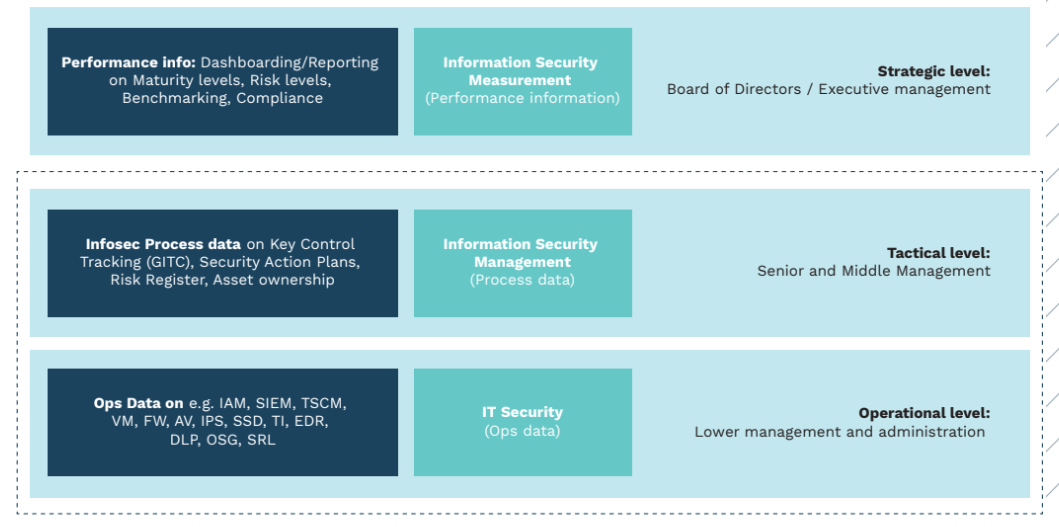
\includegraphics[scale=0.35]{Figures/stakeholders.png}}
    \caption{Cyber Security Stakeholders at Functional levels.}
    \label{fig:stakeholders}
\end{figure}
\FloatBarrier
The stakeholders
at a strategic level 
can be board of directors or an executive management, 
for example a Chief Information Security Officer (CISO) 
who is responsible for security related compliance 
and eventually also for its legal implications
\citep{farnham2013tools}. 
For a CISO, 
a cyber intelligence place them in an elevated knowledge zone 
of known risks 
and help to prepare their strategic decisions 
to tackle the potential risk,  
safeguarding and protecting the digital assets 
and safeguarding and protecting the business information. 

Tactical level stakeholders
transforms the strategic decisions to operational tasks 
and help Operational level to execute tasks 
for protection of digital assets and business information
\citep{farnham2013tools}.

\section{Problem Definition}

In this section, I have explicate the problem by first
explaining about the challenges being faced by the stakeholders in detail and then the over all implication of the problem on the stakeholder’s organisations. 
And lastly the impact if it does not get addressed.

\subsection{Problem}

The current status quo 
is that cyber news or cyber information 
are being pushed via multiple media 
\enquote{RSS, mail, WWW, news feeds etc} 
to multiple stakeholders of an organisation  
in a scattered way 
\citep{schales2011stream}
and are manually interpreted (see FIGURE \ref{fig:problem2}), 
this causes a dilute and incomplete picture 
\citep{liao2016acing}. 
Especially in a world where threats emerge 
in numbers and sophistication. 
In 2018 there where one billion unique malware samples counted
\citep{kucuk2020deceiving}.

\begin{figure}[ht]
    \centering
    \fbox{
\includegraphics[width=0.4\linewidth]{Figures/problem2.png}}
    \caption{Problem with information from multiple feeds. }
    \label{fig:problem2}
\end{figure}

\subsubsection{Impacted Stakeholder}

Stakeholders at every level faces problems 
with respect to cyber information and cyber intelligence
\citep{tounsi2018survey}. 
Stakeholders misses the fine link 
between cyber information and cyber intelligence 
due to volumetric issues, 
due to lack of contextualisation, 
due to lack of insight, 
due to lack of clear language and 
due to lack of advice \citep{barnum2012standardizing}.
Stakeholders concerns at each level are discussed below.

\subsubsection{Concerns at Strategic Levels}

The essence is to be aware of the latest news on cyber crimes 
and security breaches 
which can have legal implications. 
Here they face the problem of the need to scan 
the cyber newsfeed over thousand of intel sources 
before they can transform any cyber information into cyber intelligence.

\subsubsection{Concerns at Tactical Levels}

Their focus is to define the security action plans 
for the digital assets they hold the accountability. 
Here they have the problem to find the cyber information 
which is relevant to their digital assets and lack of advice. 

\subsubsection{Concerns at Operational Levels}

Their focus is to protect IT systems 
by taking required actions against the known threats 
and vulnerabilities 
defined in the security action plans; provided by the tactical level. 
Here they have the problem of time consumption 
for identifying systems, IOCs and solution analysis.

\begin{figure}
\centering
    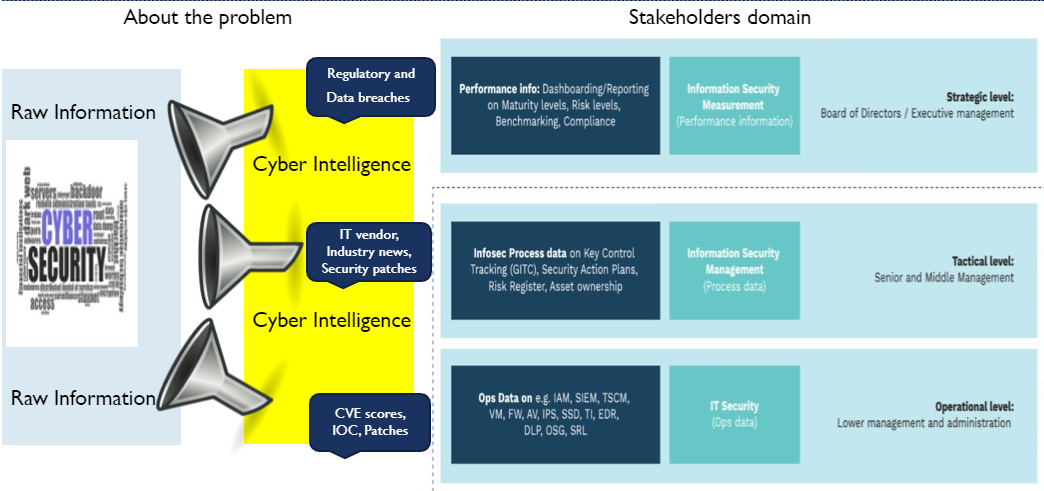
\includegraphics[scale=0.60]{Figures/stakeholder-problem.png}
    \caption{Stakeholders concerns at respective levels.}
    \label{fig:stakeholder-problem-domain}
\end{figure}


\subsection{Problem Statement}

There are Paid Sources and Open Sources to collect cyber information or cyber newsfeed into cyber intelligence platform- ‘Cyber-All-Intel’. ‘Cyber-All-Intel’ takes as input cybersecurity related text data from various unstructured sources like Dark Web, blogs, social media, National Vulnerability Databases (NVDs), newspaper articles, etc \citep{mittal2019cyber}. Other similar tools like 
Taranis\footnote{About Taranis \url{https://github.com/NCSC-NL/taranis3/wiki}}, 
IntelMQ\footnote{About IntelMQ \url{https://github.com/certtools/intelmq}}
and 
C1fApp\footnote{About C1fApp \url{https://www.c1fapp.com/}} 
are designed to collect, process and extract threat intelligence from open sources to obtain actionable cybersecurity information for the security analyst and advisors. 

\bigbreak

\textit{\textbf{But these tools require certain automations and efficient algorithms to filter, co-relate and tagging logics to make relevant cyber newsfeeds which get collected from over thousand of newsfeeds sources. 
And, it is difficult for stakeholders to manage enormous sources and exponentially available cyber information manually. 
This ultimately impacts the pace required to keep up to date with the Cyber threat Intelligence. 
Scanning all threats from all sources is tedious 
\citep{ghazi2018supervised} and most important is to transform and customize news feeds to make relevant for an organization in a specific sector, so that it could be operational and useful.
}
}

%----------------copy from res %question-------------------------------%-----------------------------------------------
\section{Research Question}\label{Research Question}
The scenario here is to transform the retrieved cyber threat information from multiple sources into organisation-specific cyber newsfeed intelligence. Would it be beneficial for the stakeholders if,  we could design a prototype artefact 1) to filter the cyber newsfeed into a specific context, 2) to tag relatable cyber newsfeeds data, and 3) to overcome the volumetric problem of sources for transforming cyber newsfeed into cyber intelligence?

As an example; given any vital sector
\citep[table 2]{luiijf2003critical} like water, housing, finance and hospitals, the companies who are subjective to EU directives\footnote{Directive (EU) 2016/1148 of the European Parliament and of the Council of 6 July 2016 concerning measures for a high common level of security of network and information systems across the Union: \url{http://data.europa.eu/eli/dir/2016/1148/oj}} would like to receive  cyber intelligence related to their digital landscape.

%\footnote{\url{https://en.wikipedia.org/wiki/Water_industry}}
\bigbreak
\textbf{How can we create a prototype, for filtering organisation-specific contextual cyber newsfeed, for tagging organisation-specific relatable cyber newsfeed, and for assessing the quality of the cyber newsfeed data sources; which can be validated by the stakeholders?}

\subsection{Sub-research questions}\label{Sub-research question}
To answer the aforementioned research question, we need to disseminate the research question into logical  sub-research questions to focus on granular details. With this problem  in mind, I  define three sub-research questions:

\begin{enumerate}
    \item What are elements in a cyber newsfeed processing chain and what are the parameters for automation?
    \begin{enumerate}
        \item What are the core concepts of cyber newsfeeds and how do they work according to the literature?
        
        \item How does the vendor field of automated cyber newsfeed suppliers of artefacts look like according to the literature?
    \end{enumerate}
    

    \item How to make a prototype to filter contextual cyber intelligence, perform automatic relevance tagging and perform analysis for risk determination and advisory?
    
    \item How to make a prototype for assessing the quality of the data sources?
    
    \item How to get the prototype validated for \emph{both 1) the design and 2) the output of this artefact} by the stakeholders of the specific organizations?
\end{enumerate}


\subsection{Research Deliverables}
An Implemented prototype artefact
for converting the cyber newsfeeds  
into relevant and contextual cyber intelligence 
based on  organisational-specific context 
and tags 
with results duly validated by the stakeholders.

\begin{enumerate}
   \item For Sub-research Question 1a and 1b: A literature review to explore the core concepts in the field of cyber newsfeed and   a literature review to explore the available artefacts.
       
  
    
    \item For Sub-research Question 2: 
    \begin{itemize}
        \item  A prototype which will have modules or sub-modules for collection, processing, analysis, publication and collection of user feedback. This is in chapter \ref{Chapter8_artefact-design}, section \label{New artefact prototype}, \nameref{New artefact prototype}.
        \item Power point presentation to the Cyber Analysts. Presentation listed in appendix \ref{Presentation to on2it}.
        \item Tool demonstration to the Cyber Analysts. It is in Chapter \ref{Chapter9_artefact-evaluation}, \nameref{Chapter9_artefact-evaluation} in section \ref{Demo Link},  \nameref{Demo Link}.
        
    \end{itemize}
    
   
     \item For Sub-research Question 3: A prototype to access the quality of data sources. This is presented in chapter \ref{Chapter8_artefact-design} section \ref{quality_source}, \nameref{quality_source}.
    \item For Sub-research Question 4:
    \begin{itemize}
    \item A demo of the simulated prototype and evaluation  report from the Focus group. Demo is in chapter  \ref{Chapter9_artefact-evaluation}, \nameref{Chapter9_artefact-evaluation} in section \ref{Demo Link} and evaluation report is in chapter \nameref{Chapter9_artefact-evaluation}, section \ref{Artefact Evaluation Results}, \nameref{Artefact Evaluation Results}. 
     \item Power point presentation to the Focus Group. Presentation listed in appendix  \ref{Presentation to GSS}.
        \item Tool demonstration to the Focus Group. It is in Chapter \ref{Chapter9_artefact-evaluation}, \nameref{Chapter9_artefact-evaluation} in section \ref{Demo Link},  \nameref{Demo Link}.
        \item Power point presentation to the CEO of a cybersecurity company. Presentation listed in appendix \ref{Presentation to CEO}.
       
     \end{itemize}
\end{enumerate}
The prototype was developed as a simulator software in coordination with ON2IT research department. An output of this simulation will be verified for the relevancy and actionability in the context of stakeholder’s interest.

\section{Conclusion}
With the end of this chapter, I have tried to help readers to get familiar with the problem background, and to understand the problem context; and expectations from this research work.








 
%% Chapter 5

\chapter{Research question} % Main chapter title

\label{Chapter5_research-question} % For referencing the chapter elsewhere, use \ref{Chapter5} 

%----------------------------------------------------------------------------------------

The scenario here is about the retrieving cyber threat information to transform into cyber intelligence over various different sources. Would it be beneficial for the stakeholders if,  we could design an prototype artefact 1) to overcome the volumetric problem of sources, 2) to filter the cyber newsfeed into a specific context, and 3) to tag relatable data stream for automatic risk determination?

As an Example: For any vital sector\citep{luiijf2003critical}[table 2] like water\footnote{\url{https://en.wikipedia.org/wiki/Water_industry}} industry, may only like to receive water industry-specific cyber newsfeeds. A water industry may not be interested in hospital or oil or any other industry-specific cyber newsfeeds. 
\bigbreak
\textbf{How can we create a prototype, for assessing the quality of the cyber news data sources, for filtering contextual cyber newsfeed, for tagging relatable cybernews feed stream, cybernews Correlation, for performing Relevance tagging and Automated Risk Determination, which can be validated by the users of the artefact to make it relevant for a specific organization?}

\section{Sub-research question}
To answer the aforementioned research question, we need to disseminate the research question into logically  sub-research questions to focus on distinct part of prototype to make it beneficial for usages. With this problem field in mind we define three related sub-research questions:

\begin{enumerate}
    \item What are elements for a cybernews feed assessment method and what are the parameters for automation?
    \begin{enumerate}
        \item What are the core concepts of Cybernews feeds and how do they work according to the literature?
        
        \item How does the vendor field of automated cybernewsfeed suppliers of artefacts look like according to the literature?
    \end{enumerate}
    
    \item How to make a prototype for assessing the quality of the data sources?

    \item How to make a prototype to filter contextual cyber Intelligence, perform automatic relevance tagging and perform analysis for automated risk determination and advisory?
    
    \item How to get the prototype validated for \emph{both 1) the design and 2) the output of this artefact} by the end users of specific organizations?
\end{enumerate}


\section{Research Deliverable:}
An Implemented prototype for converting cyber newsfeed or cyber information into relevant and contextual cyber intelligence based on parameterized context and tags with results duly validated by end users.
\begin{enumerate}
    \item For Sub-research Question 3: A prototype which will have modules or sub-modules for collection, processing, analysis, publication and collection of user feedback.
    \item For Sub-research Question 2: A prototype to access the quality of data sources.
    \item For Sub-research Question 4: A demo of the simulated prototype and validation report from group of experts.
\end{enumerate}

This prototype was developed as software in coordination with ON2IT research department. An output of this simulation will be verified for the relevancy and actionability in the context of stakeholder’s interest.


 
% Chapter 6

\chapter{Research Approach} % Main chapter title

\label{Chapter6_research-approach} % For referencing the chapter elsewhere, use \ref{Chapter6} 

\section{Introduction }
This chapter covers the approach taken to select the research methodology and factors considered in selecting the research methodology. After exploring different research methods in 
\citep{recker2012scientific}, 
I found that Design Science Research (DSR) methods would be the most appropriate method in this thesis. 
The detailed reasoning about the research approach 
(FIGURE \ref{fig:Research Flow})
is explained in further sections of this chapter.

\begin{figure}[ht]
    \centering
    \fbox{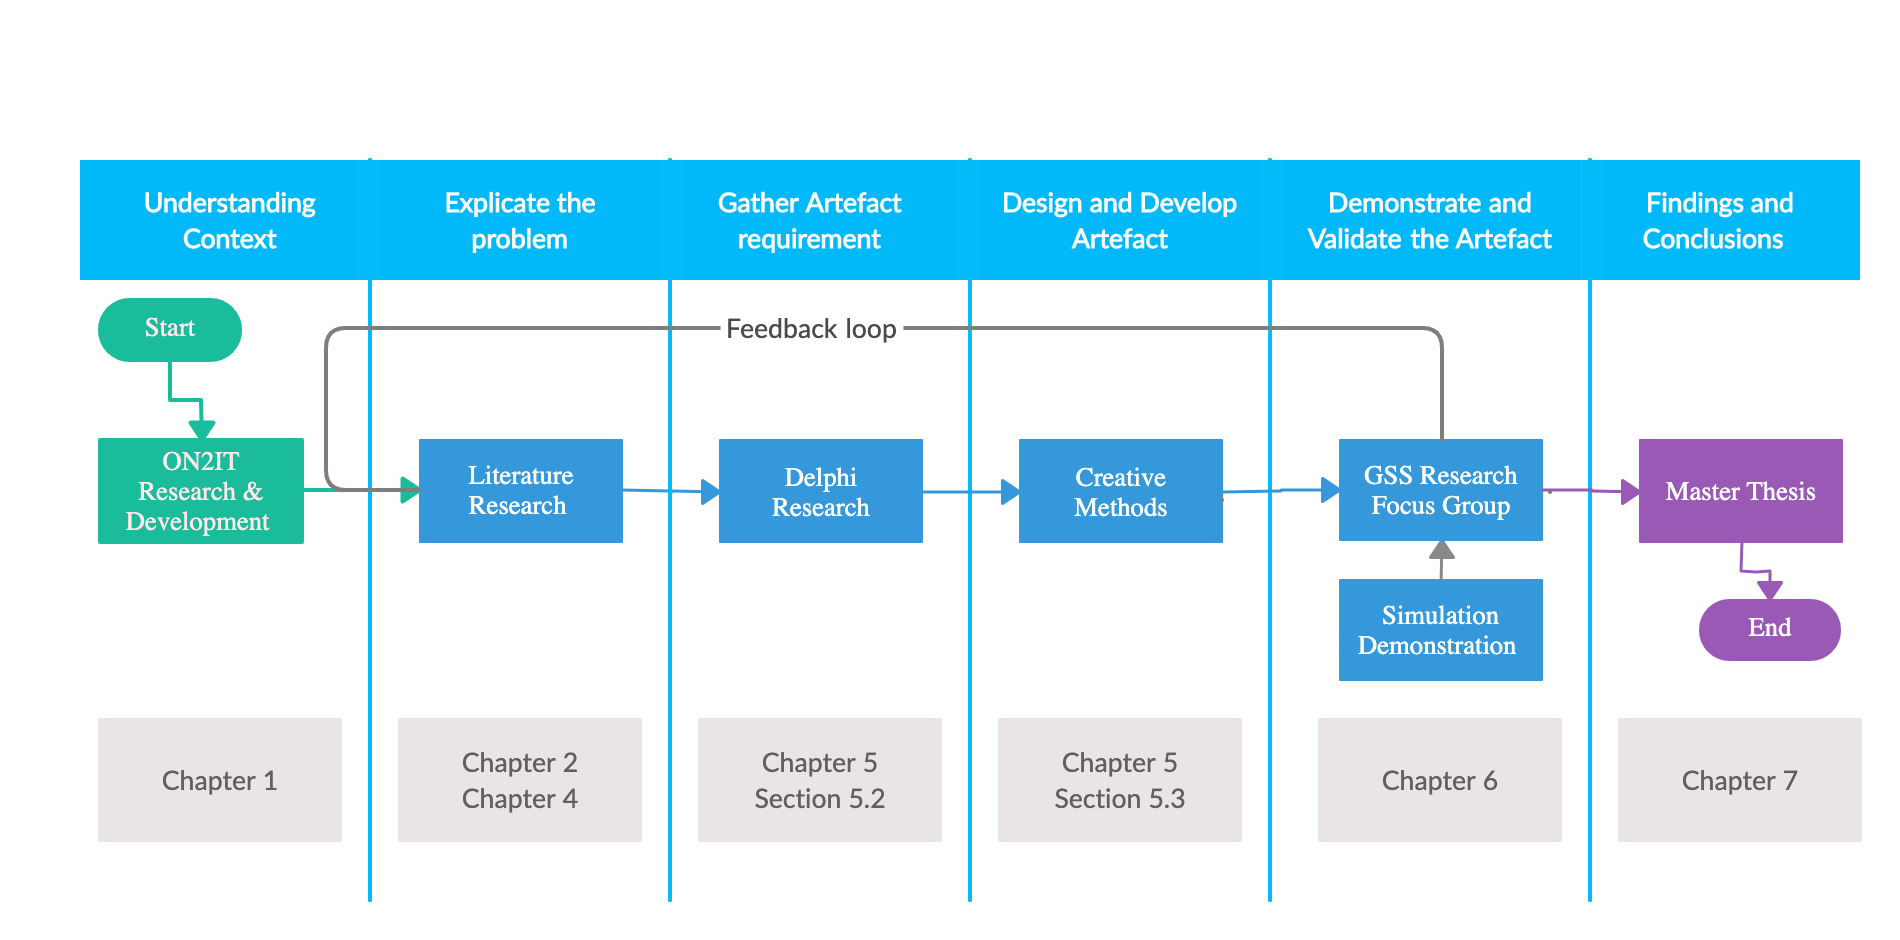
\includegraphics[width=1\linewidth]{Figures/Research Flow.png}}
    \caption{Research Approach and Structure of the thesis}
    \label{fig:Research Flow}
\end{figure}
\section{Research Methodologies } 

To determine the research methodology for the research process, 
I have examined the following four research methods:  
Quantitative, Qualitative, Mixed Methods and Design Science Research (DSR)
\citep{recker2012scientific}.

\subsection{Research Methodologies According to Scientific Research in Information Systems}

I summarize the methods as following:

\begin{enumerate}

    \item The Quantitative Methods are used to uncover truth using data collection as scientific evidence.
    
    \item The Qualitative Methods are used to explore social and cultural phenomena using texts for data interpretation.
 
    \item The Mixed Methods and used to combine both Qualitative and Quantitative for generating as well as testing the grounded theory.
    
    \item The Design Science Methods (DSR) are used to describe artificially crafted solutions for the design problems.
    
\end{enumerate}

%In an attempt to define my research methodology, I have evaluated all the four research methods proposed by the author \citeauthor{recker2012scientific}, in his book \citep{recker2012scientific}. Based on the reasoning provided by the author, I found that:
\subsection{AMS Guidelines}
I have also considered the recommendation from AMS regarding the master thesis project as depicted  in FIGURE \ref{fig:relevance-rigor}. 

\begin{figure}[ht]
    \centering
    \fbox{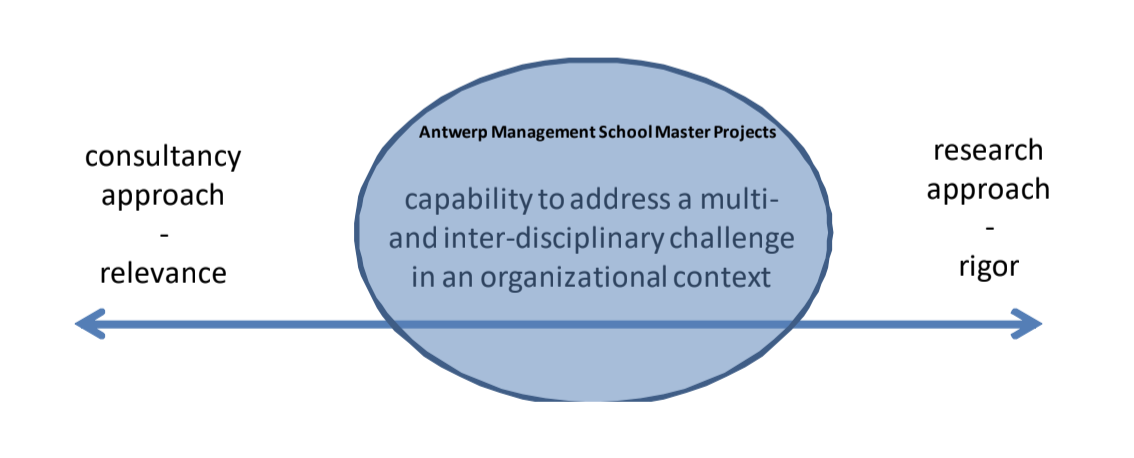
\includegraphics[width=1\linewidth]{Figures/relevance-rigor.png}}
    \caption{Balancing both rigor and relevance}
    \label{fig:relevance-rigor}
\end{figure}
\begin{quote}
`As we do adhere to
balancing both rigor and relevance, recommendations coming out of the master project should be
practical in nature and most relevant for organizations.` 
- Antwerp Management School
\end{quote}

\begin{figure}
\centering
    \includegraphics[scale=.75]{Figures/dsr.png}
    \caption{DSR  Cycle \citep[p. 80]{hevner2004design}}
    \label{fig:dsr }
\end{figure}

\section{Why Design Science Research?}
\label{Research Methodology: Design Science Research}

Since I wanted to explore methods to solve the problem at hand of absence of actionable news, 
I have chosen a research approach that does just that. First explicating the problem, 
than drafting requirements and than  establishing the prototype artefact that can be validated by the target group 
\citep{bobbert2018improving}.  
Considering the research requirements of building an artefact using rigor and relevance, 
I have concluded that it cannot be achieved  by  other methods but DSR.

\subsection{Factors consideration}

After evaluating DSR for my research which is about crafting a new artefact, 
I found that DSR Methods would guide best in the given factors of:

 \begin{enumerate}
     \item Stakeholders needs of cyber newsfeed.
     \item Building and Evaluating the Artefact.
     \item Application of existing knowledge.
     \item Balancing both rigor and relevance 
     (AMS recommendation)
     FIGURE \ref{fig:relevance-rigor}. 
 \end{enumerate}
 
\subsection{Additional consideration}

According to \cite{march1995design}, 
use of DSR methods are prominent to build and evaluate an artefact.
I would endorse my selection of using DSR methods 
to create and evaluate  Model, Method and Instantiation 
as shown is (TABLE \ref{table:research-activity}), 
where our requirements of creating an artefact 
highly resonates with the Design Science methods (DSR).

%% This file contains only a table.
%% this file is included into Chapter8

\begin{table}[bp]
   \setlength{\arrayrulewidth}{0.1mm}
    \setlength{\tabcolsep}{3pt}
    \renewcommand{\arraystretch}{1.5}

    \centering{}
 
    \caption{Research activities and outputs 
    adapted from \citep{march1995design}}
    \label{table:research-activity}
    
    \begin{tabularx}
    {\columnwidth}{|l|l|X|X|X|X|} 
    
%    |a|>{\columncolor[HTML]{FFFFFF}}C|C|C|
     \arrayrulecolor[HTML]{06000A}
        %% Table Body
       
        \hline
         \rowcolor[HTML]{FFFFFF}& & Constructs & Model & Method & Instantiation \\
        \hline
   
\cellcolor[HTML]{ECB4E8} &Build	&  	\multicolumn{1}{c|}{ \cellcolor[HTML]{ECB4E8} ---- }& \cellcolor[HTML]{ECB4E8}$X$ & \cellcolor[HTML]{ECB4E8}$X$ & \cellcolor[HTML]{ECB4E8}$X$	\\    \cline{2-2}\cline{4-6}
\multirow{-2}{*}{\cellcolor[HTML]{ECB4E8} \textbf{Design Science}} & Evaluate & 	\multicolumn{1}{c|}{ \cellcolor[HTML]{ECB4E8}----}&  \cellcolor[HTML]{ECB4E8}$X$ & \cellcolor[HTML]{ECB4E8}$X$ & \cellcolor[HTML]{ECB4E8}$X$
		\\  \hline 

\cellcolor[HTML]{BFCEED} &Theorize	& 	\multicolumn{4}{c|}{ \cellcolor[HTML]{BFCEED} --Not Applicable--}	\\  \cline{2-2}
\multirow{-2}{*}{\cellcolor[HTML]{BFCEED} \textbf{Natural Science}} & Justify & 	\multicolumn{4}{c|}{ \cellcolor[HTML]{BFCEED}--Not Applicable--}	\\   \hline


    \end{tabularx}

\end{table}








 \FloatBarrier

\section{Design Science Research Components}

Literature review, Delphi research, Creative process and 
GSS research are the DSR components applied in this research work.
I have explored the paper
\citep{bobbert2017defining} and  
\citep{bobbert2017exploring}. 
In these papers, the author has examined different research methods for designing and engineering an artefact. 
\cite{bobbert2017exploring} states that 
Design Science Research (DSR) (FIGURE \ref{fig:dsr }) 
Strategy advocates triangulation of different research methods 
within DSR to be applied during multiple research phases. 
Different research methods used during this research are listed below. 

\begin{enumerate}
    \item To explicate the problem: 
    I have used Literature Research to gain insight on the existing work on cyber newsfeed related work according to academic literature. Further, to gather the requirements from users, in this case cyber analysts.
    
    \item To gather requirements: 
    I have used Delphi Research methods
    \citep{linstone1975delphi}, ON2IT agile ceremonial events like: stand-ups(twice a week), short calls, multiple meetings with the team and exclusive individual interactions were planned to collect and refine the requirements.
    
    \item To design and develop the prototype: 
    Creative Process
    \citep{mednick1962associative} 
    was used.
    
    \item To demonstrate and validate the prototype: 
    Group Support System (GSS) research for validating the artefact 
    in order to execute DSR since validating is hard and complex 
    \citep{arnott2010relevant}. 
    For validation we planned to took an overall perspectives and experiences of the Strategic, Tactical and Organizational level
    \citep{Bobbert-Y-2019} functions or stakeholders. 
    The group (six to eight) would discuss on specific topics and the questions would be designed for free expression.
   
\end{enumerate}
 If I am looking at the combinations in the DSR, I am using multiple research applied by \cite{bobbert2017exploring} for an artefact creation as shown TABLE \ref{table:GSS}.


%% This file contains only a table.
%% this file is included into Chapter8

\begin{table}[ht]
    \setlength{\arrayrulewidth}{0.1mm}
    \setlength{\tabcolsep}{4pt}
    \renewcommand{\arraystretch}{1.0}
    
    \centering{}
    
    \caption{GSS Contribution in BIS Artefact adapted from \citep{bobbert2017exploring}}
    \label{table:GSS}
    
    \begin{tabularx}{0.96\linewidth}{|>{\columncolor[HTML]{ECB4E8}} p{1.5cm}|p{11.55cm}|} 
    
%    |a|>{\columncolor[HTML]{FFFFFF}}C|C|C|
    \arrayrulecolor[HTML]{06000A}
    
        %% Table Body
        \hline
       
         \rowcolor[HTML]{BFCEED}     
         \textbf{Type of research within DSR} 
         & 
         \textbf{Contribution to designing and engineering a Business Information Security artefact}
         \\
        \hline
        Literature research 
        &
        Explicating and defining the problem in a systematic, structured way. Objectivity removes the
        element of Fear Uncertainty and Doubt (FUD). Unbiased, structured point of departure for the
        design cycle. Requires a certain level of expertise in the topic.
         \\
        \hline
        Delphi research
        &
        Anonymous inventory and selection of views and standpoints (preferably based upon
literature data). Rigorous examination process for scrutinizing the problem via, for example,
expert opinions. Collecting global views on criteria requirements with the use of technology.
Knowledge sharing. Enables double loop learning via multiple iterations. Automated. No
geographical limitations. Limited in group interaction and discussion.
         \\
        \hline
        Group Support System research 
        & 
        Enables to create, share and capture knowledge as well as design items.
        Stimulates design thinking and stakeholder collaboration due to the “group element”. 
        Ability to collect, assess and select product requirements in a very short time frame. 
        Supports the regulative process of testing and validating requirements. 
        Processing large data sets.
        Double Loop learning. 
        Bridging knowing-doing gaps. 
        Stimulating group dialogues (i.e. among Boards of Directors and Management teams).
        Makes it possible to establish group consensus. 
        Supports the decision making process. 
        Threat of the “law of the decibel”. 
        Requires professional group moderation skills.  	
        \\
       \hline
    \end{tabularx}

\end{table}









 \FloatBarrier



\section{Research Flow}
In FIGURE \ref{fig:Research Flow}, the research flow and related research work with the link to the Chapters in this book can be visualised.

 

%---------removed pic, used tab----
%\begin{figure}
%\centering
%    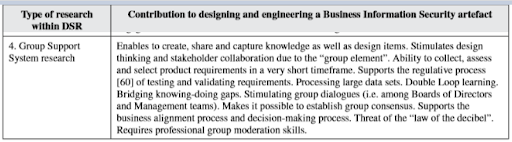
\includegraphics[scale=0.60]{Figur%es/GSS.png}
%    \caption{GSS contribution in BIS %Artefact }
%    \label{fig:GSS }
%\end{figure}
%---------removed pic, used tab----
\section{Conclusion}

Thus, along with the DSR framework, Literature review, Delphi research, Creative process and 
GSS research methods  are used to create requirements,
demonstrate and validate the  artefact's first version.
 
 
% Chapter 7

\chapter{Literature Review} % Main chapter title

\label{Chapter7_literature-review} % For referencing the chapter elsewhere, use \ref{Chapter7} 

\section{Introduction }
This chapter is answer to the sub research question 1. 
In this chapter, first mention 
is about the literature search approach 
and then a literature review was done to understand the current state of available artefacts according to the literature. 
It helped to find the gaps between the available artefacts 
and the desirable artefacts. 

From the collected academic work, 
the existing knowledge on cyber newsfeed assessment process 
and related concepts like people, practices, 
guidelines and methods available according to academic literature 
(sub research question 1a) are listed. 
It also illuminate about the vendor field of automated cyber newsfeed suppliers of the artefacts (sub research question 1b).  
Collected literature has been used to explore the following topics.

\begin{enumerate}
    \item Existing practices, systems, and people involved in automated cyber newsfeed.
   
    \item Existing guidelines on cyber newsfeeds correlation, contextualization, and analytics. 
    
     \item Existing methods available for data source quality assessment.
\end{enumerate}

\section{Approach}

I have searched the knowledge body in different sources and some knowledge was acquired during the discussion with ON2IT cybersecurity professionals. 
The primary sources of knowledge included academic publications, textbooks, research papers in journals and conferences. The additional sources of knowledge exploration were online magazine articles, white papers, websites, and artefact manuals. 
Exclusive details about the publication year criteria, used keywords and the libraries are listed below.
\begin{enumerate}
    \item  Filter on \textbf{year greater than 2010} to make it relevant.
    \item  The important keywords used for the search used 
        \textbf{cyber, security, threat, news, intelligence, live, RSS, news, feed, system, artefact, people, cyber experts, information, intel} or \textbf{feeds}.
    \item  Libraries used for academic papers: \textbf{Google Scholar} and \textbf{Web of Science}.
    \item  Search String formulation:\textbf{cyber +(security|threat|news|intelligence) + [(live|rss|news)]+ [Feed[s]]}.

\end{enumerate}

The above search string will follow the following match pattern shown as an example in the TABLE \ref{tab:search-pattern}.



\begin{table}
    \caption{Illustration of search pattern: Literature Search Analogy}
    \label{tab:search-pattern}
    \centering{}
   \resizebox{\textwidth}{!}{
    \begin{tabular}{|l|l|l|l|}
    \toprule
      \rowcolor[HTML]{BFCEED} 
    \textbf{Symbol} & \textbf{Meaning X} & \textbf{Example } & \textbf{Interpretation} \\
    \midrule
    {[]} & Zero or One Occurrence of the string or character within square bracket & [Feed] & “Feed” or null \\
    {[ ]} & Zero or One Occurrence of the string or character within square bracket & [s] & “s” or null\\
    ( ) & One Occurrence & (Security) & Security \\
    | & Optional & live|rss & either “live” or “rss”\\
    + & And & cyber + security & “cyber” and “Security” both \\
    \bottomrule
    \end{tabular}
}
\end{table}

\section{Overview of the literature search}
I explored 52 papers using snowball \citep{wohlin2014guidelines} approach and the majority of those papers are re-used and lined up in  bibliograpy \ref{sec:bibliography}. 



\section{Existing practices, systems, and people involved in automated cyber newsfeed}\label{Existing practices, systems, and people involved in automated cyber newsfeed}


In this section the existing literature about the practices, systems and people involved has been covered to explain the existing environment in which cybersecurity world and cyber newsfeed are interrelated. 
The first section \ref{Existing-practices}, \nameref{Existing-practices} deals with the generic practices involved in cybersecurity world and how cyber newsfeed is important to such practices in cybersecurity world. 
The second section \ref{Existing systems}, \nameref{Existing systems} and third  section \ref{People}, \nameref{People}  deal with the relation and importance of systems and people involved in cyber security world and how is cyber newsfeed is importance to them. 

\cite{sector10itu} states that cybersecurity is the collection of tools, policies, security concepts, security safeguards, guidelines, risk management approaches, actions, training, best practices, assurance and technologies that can be used to protect the cyber environment and organization and user’s assets. 

Organization and user’s assets include connected computing devices, personnel, infrastructure, applications, services, telecommunications systems, and the totality of transmitted and/or stored information in the cyber environment.

Cybersecurity strives to ensure the attainment and maintenance of the security properties of the organization and user’s assets against relevant security risks in the cyber environment 
\citep{sector10itu}. 
The general security objectives comprise the following: Availability Integrity, which may include authenticity and non repudiation Confidentiality 
\citep{sector10itu}.



\subsection{Existing practices}\label{Existing-practices}

With the rapid growth in use of Information Technology, organizations are getting very vigilant when it comes to protecting business information. Form simple security solutions (e.g., anti-virus software and firewalls) to complex security solution (e.g., 3G\footnote{3G or Application firewall \url{http://www.avolio.com/papers/FWTKv1.0Announcement.html}} firewalls), organizations are doing the best possible security investment and management \citep{yeh2007threats}. 
At the same time the cyber attackers are continuously trying to invent new ways of attacking IT systems and their approach to attack vulnerabilities has also evolved over time \citep{jang2014survey}. 

This means that as an organization, one cannot ensure 100 percent guarantee of secure IT systems. Despite putting a lot of effort on safeguarding and securing organizational assets, there are high chances of getting exposed to any unpredictable security incident. In such unpredictable situations, to avoid cyber security incidents, keeping an eye on daily updates happening in dark web is very important \citep{chen2006intelligence}. 
Such cyber information related about information security, new threats, vulnerabilities, security products, and research is available on internet with open access \citep{fogelman2008mining}. These information can be used in many ways and
 \cite{zimmerman2014ten} provides 10 strategies to handle such cyber information.

\begin{itemize}
    \item \textbf{Cyber Intel Collection:} Collection and consumption of cyber intelligence reports, cyber intrusion reports, and news related to information security, covering new threats, vulnerabilities, products, and research. 
    
    \item \textbf{Cyber Intel Analysis:} Analysis is done manually by security analysts or by automatically by some security vendors, in some organization they use in house cyber news analytics system.

    \item \textbf{Cyber Intel Distribution:} Post analysis redistribution of cyber intelligence reports, cyber intrusion reports, and news related to information security to members on either a routine basis such as a weekly or monthly cyber newsletter or a non-routine basis such as an emergency patch notice or phishing campaign alert. 
    
    \item \textbf{Cyber Intel Creation:} In case of newly observed threat based on primary research analysis of a new threat or vulnerability, the result of research is shared with larger audience of potential beneficiaries.
    
    \item \textbf{Cyber Intel Fusion:} Extracting data from cyber intel and synthesizing it into new signatures, content, and understanding of adversary Search Results. Tactics, Techniques and Procedures (TTPs), thereby evolving monitoring operations 
    (e.g., new signatures or Security Information and Event Management (SIEM) content). 
    
    \item \textbf{Trending:} Long-term analysis of event feeds, collected malware, and incident data for evidence of malicious or anomalous activity or to better understand the constituency or adversary. For analogy any information on phishing email about COVID-19 and privacy concern in online meeting tools were trending during Feb-2020 to Apr-2020. 

    \item \textbf{Cyber Threat Assessment:} An estimation of potential threats on existing IT systems. This is often performed in coordination with other cybersecurity stakeholders. 
\end{itemize}

\subsection{Existing systems for Cyber Intelligence Sharing}\label{Existing systems}
This section is about the explored systems, according to existing literature which are associated with cyber newsfeed collection, processing and production. 
A generic term for such systems would be \textbf{Cyber Threat Intelligence Sharing Platforms}.
These systems when used in practice provides operational mechanisms to support the exchange of intelligence on cyber security threats and incidents amongst different entities \citep{brown2015cyber,sauerwein2018shadow}.  The related systems types has been presented here below is based on 1) Systems producing or publishing cyber newsfeed on Internet and 2) Systems consuming or collecting cyber newsfeed from Internet.

\begin{itemize}
    \item \textbf{Systems producing cyber newsfeed:} 
    This includes all the sources that are potential supplier of the cyber newsfeed items. 
    Websites, Emails, Partner feeds and Social media feeds. These sources are owned by Computer Emergency Response team (CERT) organizations, Cyber Security Organizations or National Security organizations. 
    Some cyber newsfeed items are also shared by Original Equipment Manufacturer (OEM) like Palo Alto, Microsoft and Oracle. 
    There are some websites managed by cyber security researchers, those individual who are dealing independently in cyber security domain and continuously contribute to Cyber Defense. 
    These systems are generally accessible without authentication and are open to use. 
    Some systems may require authentication like account or subscriptions to get the cyber newsfeed items. 

    \item \textbf{Systems consuming cyber newsfeed:} 
    In this section, we will see all the systems and their properties which are involved once the cyber newsfeed item is generated and systems which are involved in collection of cyber newsfeed and then transforming cyber newsfeed items to a valuable, actionable and quality cyber intel. 
    Once a cyber newsfeed item is published at any website, it needs to be collected and analyzed to check its usefulness for the purpose of cyber intel.
    The setup of such systems varies from each other and has been designed for specific purpose.
    We have searched the web to find the list of systems and evaluated so for on the basis of functionalities, support factor, and distribution type. Refer to TABLE \ref{tab:tip-list} for the available systems consuming cyber newsfeeds.

 
\end{itemize}


\begin{table}[hbt!]
 \arrayrulecolor[HTML]{06000A}  
\caption{Assessed List of Threat Intelligence Platforms }
\label{tab:tip-list}
\centering
\resizebox{\textwidth}{!}{\begin{tabular}{|>{\columncolor[HTML]{ECB4E8}}p{3.3cm}|p{8.3cm}|p{2cm}|p{1.7cm}|p{1cm}|p{1.7cm}|}
 \hline
 \rowcolor[HTML]{5789F3} 
 \multicolumn{6}{|c|}{ \textbf{List of TIP applications explored} } \\
 \hline
  \rowcolor[HTML]{BFCEED} 
 Application & Brief Overview & \multicolumn{4}{c|}{Maintainability Parameters } \\

 \hline
 \textbf{Name} & \textbf{} & \textbf{Distribution} & \textbf{Support Forum?} & \textbf{Active years} & \textbf{Last Issue resolved}\\

 \hline
 
 CimSweep & Ability to perform incident response and hunting operations & Open Source & Yes & 4 & Sep 2017\\
 \hline
GRR Rapid Response - & The goal of GRR is to support forensics and investigations & Open Source & Yes & 9 & Apr 2020\\
\hline
TheHive - & Security Incident Response Platform, tightly integrated with MISP & Open Source & Yes & 2 & May 2020\\
\hline
Osquery - & The tools make low-level operating system analytics and monitoring both performant and intuitive. & Open Source & Yes & 6 & Apr 2020\\
\hline
MISP: Open-source threat intelligence platform & Used to store, share, collaborate on cyber security indicators & Open Source & Yes & 9 & May 2020\\
\hline
CRITs:Collaborative Research Into Threats & A good collaboration tool but CISCO will stop Grant in 2020 & Open Source & Yes & 10 & Jul 2019\\
\hline
MANTIS & Model-based Analysis of Threat Intelligence Sources & Open Source & Not Maintained & 7 & May 2018\\
\hline
CIF & Combined with machine learning to produce unified threat feeds & Open Source & Yes & 1 & Apr 2020\\
\hline
ThreatGrid: & Sandboxing with threat intelligence into one unified solution & Cisco & PINA & PINA & PINA\\
\hline
LookingGlass: & Third party risk monitoring & Looking Glass & PINA & PINA & PINA\\
\hline
Falcon Xlite & Used for end point protection & Crowdstrike & PINA & PINA & PINA\\
\hline
Verint Web Intelligence Center & HUMINT entities are operated across all web surfaces and platforms, collecting valuable information and analyzing it to transform abundant data into actionable intelligence & Sensecy & PINA & PINA & PINA\\
\hline
Anomali threatstream & with machine learning optimized threat intelligence & Anomali & PINA & PINA & PINA\\
\hline
Threatquotient & for Threat-Centric Security Operations &  & PINA & PINA & PINA\\
\hline
Threat connect & Intelligence, automation, analytics, and workflows in a single platform & Threatconnect & PINA & PINA & PINA\\
\hline
IBM® X-Force Exchange & Saas solutions with different subscription option & IBM & PINA & PINA & PINA\\
 \hline
\end{tabular}}
\end{table}
 \FloatBarrier

Based on the tools explored, I found that threat intelligence platforms are used for different purposes and are available in different formats of deployments and activity.  The most important aspects of these tools are collection because, the system cannot proceed further without having the data(cyber newsfeed) to process. 

\subsection{People}\label{People}

This section is dedicated for the cybersecurity practitioners 
and professionals dealing with cyber newsfeed and related systems. 
People are associated with a particular type of cyber security team listed below and categorized based on functional behaviour of the team.
The teams dealing with 
1) Threat Intelligence, 
2) Intrusion Detection and 
3) Incident Management 
are relevant for this paper has been therefore mentioned 
\citep{osorno2011coordinated}.

\subsubsection{Teams}

\begin{itemize}
    \item Threat Intelligence Team
    \item Security Operations Control Team
    \begin{enumerate}
       \item Computer Security Incident Response Team (CSIRT) facilitates the exchange of incident data between the three organizational roles by processing information as described in the coordinate cycle.
       \item Computer Emergency Response Team (CERT) 
   \end{enumerate}
\end{itemize}

\subsubsection{Key Activities }

According to \cite{osorno2011coordinated} following are the key activities.
\begin{itemize}
    \item \textbf{Identification} consists of recognizing events that might be associated with a cybersecurity incident. 
    \item \textbf{Act}, If the identified anomaly or event is actionable without further coordination, an organization’s identification mechanism might inform action from the response elements. 
    \item\textbf{Reporting/Directing}: Reporting is intended to communicate an organization’s understanding of an event and convey related expectations to the relevant CSIRT or organizational elements. While most identify entities report descriptive information, policy’s identification activity might provide directive guidance in terms of explicit actions to be taken. This information may be specifically targeted to the CSIRT or intended for further dissemination throughout the community via the CSIRT. 

\end{itemize}

\section{Existing methods available for data source quality assessment}
\label{Existing methods available for data source quality assessment}

\subsection{Introduction}

Given the abundance of sources, suitable metrics are required for conducting an appropriate evaluation that will help towards minimizing false alerts, as well as not missing any valuable threat information. It was found in literature that there are six qualitative parameters and 10 quantitative parameters to determine the quality of the sources.

\subsection{Date source quality assessment}

A Data source may be a source of a threat Intel or cyber newsfeed items which are published on different websites. It has been observed that the quality of information collected from the sources varies from source to source. However,  In order to determine  the quality of a threat intelligence source it is important to validate both the quality of cyber newsfeed item and the source itself. 

I have used the snowball \citep{wohlin2014guidelines} approach 
to find the applicable and latest available literature 
in the area of knowledge for the  quality of sources. 
According to \cite{mokaddem2019taxonomy}, 
a trust level can be allocated between 0 and 1 
for a source based on the image and reputation of the organization 
who owns the source. 
For example: In case a source is fully trusted, 
the source confidence is set to 1. 
If there is no trust, the source level is set to 0. 
The author of \citep{mokaddem2019taxonomy} highlights 
that calculation of Quality of source based on parameters 
could be scope of future research.

Further review of papers establishes the fact that so far 2 types of methods has been observed in the Literature: 
1) Qualitative 
2) Quantitative. 
They contribute to six Qualitative parameters and ten Quantitative parameters
\citep{schaberreiter2019quantitative}. Let’s see each of them in detail. 

% export table from table folder
%% This file contains only a table.
%% this file is included into Chapter8

\begin{table}[htbp!]
   \setlength{\arrayrulewidth}{0.1mm}
    \setlength{\tabcolsep}{5pt}
    \renewcommand{\arraystretch}{1.0}

    \centering{}
 
    \caption{Source Quality metrics: Qualitative}
    \label{table:qualitative}
    
    \begin{tabularx}{0.91\linewidth}{| p{0.5cm}|p{5.25cm}|p{0.5cm}|p{5.25cm}|} 
    
%    |a|>{\columncolor[HTML]{FFFFFF}}C|C|C|
     \arrayrulecolor[HTML]{06000A}
        %% Table Body
        \hline
        \rowcolor[HTML]{5789F3} 
        \multicolumn{4}{|c|}{Qualitative based metrics} \\
        \hline
        
        \rowcolor[HTML]{ECB4E8} \multicolumn{2}{|l|}{1 Type of Information} &
      \multicolumn{2}{l|}{4 Interoperability} \\
     
     &	1.1 Indicators	& &	4.1 Supported formats \\  
     &	1.2 Sightings	& &	4.1.1 STIX1	\\ 
     &	1.3 Courses of Action	& &	4.1.2 STIX2	\\
     &	1.4 Vulnerabilities	& & 	4.1.3 PlainText	\\
     \multicolumn{2}{|l|}{ \cellcolor[HTML]{ECB4E8}2 Provider Classification} & & 4.1.4 OpenIOC \\
    &	2.1 Data Feed Provider	& &	4.1.5 RSS	\\
    &	2.1.1 Original Provider	& &	4.1.6 JSON (non-STIX)	\\
    &	2.1.2 Aggregator	& &	4.1.7 CSV	\\
    &	2.2 Intelligent platform 	& &	4.2 Supported data exchange formats	\\
    &	2.3 Report Provider	& &	4.2.1 TAXII1	\\
    
 \multicolumn{2}{|l|}{ \cellcolor[HTML]{ECB4E8}3 Licensing Options} & & 4.2.2 TAXII2\\
 
& 3.1 Open & \multicolumn{2}{|l|}{ \cellcolor[HTML]{ECB4E8}5 Advanced API Supported}\\
&	3.2 Restricted	& &	5.1 Filtering based on dates	\\
&	3.3 Commercial	& &	5.2 Filtering based on type of information	\\
& 3.4 Information  Reuse & \multicolumn{2}{|l|}{ \cellcolor[HTML]{ECB4E8} 6 Context Applicability}\\
&	3.4.1 Commercial: Allowed	& &	6.1 Vulnerabilities \\
&	3.4.2 Academic: Allowed	& &	6.2 Threats \\
&	3.4.3 Personal: Allowed	& &	6.3 Campaigns \\
&		& &	6.4 Hashes \\
&		& &	6.5 Recommendations \\
&		& &	6.6 Incidents (Sightings) \\

      \hline
    \end{tabularx}

\end{table}











%\setlength{\arrayrulewidth}{0.5mm}
%\setlength{\tabcolsep}{10pt}
%\renewcommand{\arraystretch}{1.5}

%\newcolumntype{s}{>{\columncolor[HTML]{DDBDF7}} p{3cm}}


%\begin{tabular}{ |a | >{\columncolor[HTML]{5993C2}}c | l | b }

% \arrayrulecolor[HTML]{06000A}
% \hline
% \rowcolor[HTML]{5789F3} \multicolumn{4}{|c|}{High Level Modules = Collector} \\
% \hline
%  
%  \rowcolor[HTML]{BFCEED} Requirements: & What? & Why? & MoSCoW priority \\
% \hline
%
%Language Support	 & 	Support various languages.	 & 	To not miss intel in other languages	 & 	Must have	\\
% \hline
%Data Formats	 & 	Allow multiple data formats	 & 	To collect and process standard and recent formats	 & 	Should have	\\
% \hline
%Data Source types	 & 	Ingest from various sources	 & 	To cover broader sources of Intel	 & 	Must have	\\
% \hline
%Connection protocol	 & 	Support common protocols	 & 	To allow actual transfer To data	 & 	Must have	\\
 % 
%  \hline
% \end{tabular}
 



\subsubsection{ Qualitative Assessment}
According to \cite{schaberreiter2019quantitative}, the definition of the evaluation criteria presented in this work are based on the experiences of the authors in the H2020 project CS-AWARE, and a more extensive description of the methodology and expertise involved in defining those criteria
(TABLE \ref{table:qualitative})
is described in CS-AWARE project\footnote{\url{https://www.cyberwatching.eu/projects/959/cs-aware}} deliverable D2.2.

The Type of Information criterion indicates the type and complexity of information shared by a source. 
The Provider Classification assesses the type of ownership of the source: original or aggregator. 
The Licensing Options identifies the potential restrictions of usage for provided data. 
The Interoperability criterion assesses support for data structure formats and exchange formats, Advanced API support assesses how data can be accessed by a consumer, and Context Applicability lists different type of cyber newsfeed items.

\subsubsection{ Quantitative Assessment}
\cite{schaberreiter2019quantitative} argued that quantitative parameters can be more accurate and proposed 10 quantitative parameters as listed below in TABLE \ref{table:quantitative}. 
Along with the parameters, the description and formula is listed in the table below. Explanation of formula is not in the scope and if needed, can be referred to original author. 
The benefits of using quantitative parameters for establishing the trust of a cyber newsfeed source was acknowledged by \cite{ermerins2020scoring}. 
In this paper author used three out of 10 parameters: Extensiveness, Timeliness and Completeness for calculating a numerical  trust factors for the sources which turns to be useful.

%% This file contains only a table.
%% this file is included into Chapter8

\begin{table}[bp!]
   \setlength{\arrayrulewidth}{0.1mm}
    \setlength{\tabcolsep}{3pt}
    \renewcommand{\arraystretch}{1.0}

    \centering{}
 
    \caption{Source Quality metrics: Quantitative \citep{schaberreiter2019quantitative} }
    \label{table:quantitative}
    
    \begin{tabularx}{\linewidth}{| p{0.82cm}|p{2.50cm}|p{5.25cm}|p{1.1cm}|c|} 
    
%    |a|>{\columncolor[HTML]{FFFFFF}}C|C|C|
     \arrayrulecolor[HTML]{06000A}
        %% Table Body
        \hline
        \rowcolor[HTML]{5789F3} 
        \multicolumn{5}{|c|}{Quantitative based metrics} \\
        \hline
        
        \rowcolor[HTML]{ECB4E8} Serial \#  & Parameter type & Parameter Description & Symbol & Math Formula  \\
        \hline
 1	&	Extensiveness	&	Evaluates how many optional parameters are filled in	&	p1	&	$p1 = \frac{1}{z}\sum\limits_{n=1}^{z}(\frac{oi}{\max y_i}) $	\\ 
  \hline
 2	&	Maintenance	&	Determines how often messages are updated	&	p2	&	$p2 =  \|\frac{\frac{1}{z}\sum_{i=1}^{z}u_i}{avg(p_2s_1 \cdots p_2s_n)}\| $	\\
  \hline
3	&	False Positives	&	Determines how often messages of a source are invalidated	&	p3	&	$p3 = 1 - (\frac{{F_s}_x}{\sum_{i=1}^{n}{F_s}_i}) $	\\
 \hline
4	&	Verifiability	&	Expresses how often a source verifies the information they provide by linking their source	&	p4	&	$p4 =  \|\frac{\|\frac{1}{z}\sum_{i=1}^{z}r_i\|}{avg(p_4s_1 \cdots p_4s_n)}\| $	\\
 \hline
5	&	Intelligence	&	Indicates how much added value a source offers in their messages by linking it to other objects	&	p5	&	$p5 =  \|\frac{\|\frac{1}{z}\sum_{i=1}^{z}l_i\|}{avg(p_5s_1 \cdots p_5s_n)}\| $	\\
 \hline
6	&	Interoperability	&	Based on which data format a source provides their data in	&	p6	&	$p6 = \sum\limits_{n=1}^{n}(\frac{b_i}{n}) $	\\
 \hline
7	&	Compliance	&	Determines how compliant a source is to the standard they use	&	p7	&	$p7 =  \|\frac{\frac{1}{z}\sum_{i=1}^{z}c_i}{avg(p_7s_1 \cdots p_7s_n)}\| $	\\
 \hline
8	&	Similarity	&	Evaluates how similar specific entries of two sources are	&	p8	&	$p8 = \frac{1}{z}\sum\limits_{i=1}^{z}(y_i) $	\\
 \hline
9	&	Timeliness	&	Analyses which source provides information the quickest	&	p9	&	$p9 = \frac{1}{z}\sum\limits_{i=1}^{z}(\frac{\min t_i}{(ts)_i}) $	\\
 \hline
10	&	Completeness	&	Indicates how much of the entire world a single source represents	&	p10	&	$p10 = \frac{|B|-|A|}{|B|}$	\\
\hline
    \end{tabularx}

\end{table}






 \FloatBarrier
\section{Existing guidelines on cyber newsfeeds correlation, contextualization, and analytics}

\subsection{Introduction}
To identify and stop modern cyberattacks, 
organizations need to understand how attackers think, what they want, 
and how they work. 
It is hence essential to collect and analyze all the available information related to ongoing and previous attacks, 
and transform it into intelligence. 

\subsection{Correlation}
As observed from literature, the correlation of items from different data is a mature field. In this literature we focus on correlation techniques used in practice according to literature and the ways available for correlation. Correlating cyber newsfeed to derive similarities and meaningful relations is directly connected to natural language processing and semantics and approaches for such text analysis are based on Vector Space Models (VSMs) 
\citep{settanni2016correlating}. 
The VSM is to represent each item or data or a point, in a multidimensional space and the points which are close to each other are proved to be similar, while points that are away are less similar or entirely different 
\citep{turney2010frequency}. 
The author also claims that it is the best way so far to apply semantics.

Based on term-document VSM, \cite{settanni2017acquiring} 
proposed three custom methods, 
to correlate cyber feed or information for providing more insight and making meaningful to support cyber incident handling tasks carried out by security operation teams.

\subsubsection{Dictionary-based method}
Use of dictionary including applicable cyber words and checks if those words are part of information item.
If yes, the vector set for information is made a set of binary values.
Vector v of document d is $v_d$ = $(bf_1, bf_2, ..., bf)$, where $bf_1$= binary frequency: 0 or 1. 
This method is faster but provides a less precise correlation.

\subsubsection{Word-based approach}
In the word-based linking method we adopt as features
the documents’ own words. 
For every unique word we compute the TF (term frequency) 
and the IDF (Inverse document frequency). 
Words with an IDF below a certain empirically defined threshold 
are ignored because considered too frequent. 
TF·IDF values of the remaining n high-IDF words will determine the feature vector $v_d$ of a document d.
Advised to be used when the accuracy 
is very important and the time is not a constraint.

\subsubsection{Artifact-based method}
The raw frequency $(F_a,d)$ of a word(a) in document(d) is the total number of such occurrences within this document. 
The feature vector$(v)_d$ of the document(d) will then consist of all known artifacts.
Used to be in cases where a trade-off between precision 
and speed is necessary, this provides suitable results.

\subsection{Contextualization}
For cyber newsfeed items, 
it is important to be relevant for further course of actions. 
\cite{sillaber2016data}, highlights the problem of data quality due to vast data or cyber newsfeed coming inwards and failure to immediately find relevant and useful cyber newsfeed. 
Applying context helps cyber threat analyst to extract patterns 
or indicators representing the observable characteristics 
of specific cyber threats along with their threat context 
and relevant metadata for interpreting 
\citep{barnum2012standardizing}. 
For example, in the case of a confirmed phishing attack, 
a cyber threat analyst may harvest the relevant set of observables
(e.g., to or from addresses, actual source, subject, embedded URLs, type of attachments, specific attachment, etc.).
There are two ways of applying context 1) Manual and 2) Automated 
\citep{barnum2012standardizing}.

\subsubsection{Manually}
This includes human intensive labor, like searching in the databases or on the websites. Or discussion in group to give a context for a threat or cyber newsfeed item.

\subsubsection{Automated}
 This includes automation using machine learning algorithms and there are certain ways to automate and apply context to increase relevance \citep{wagner2017relevance}. In FIGURE \ref{fig:co-relation}, 
 we can see how a machine learning tool can be used to label a Indicator of compromise(IOC\footnote{An IOC can also come as a cyber newsfeed item.
 }). 
\begin{figure}[ht]
    \centering
    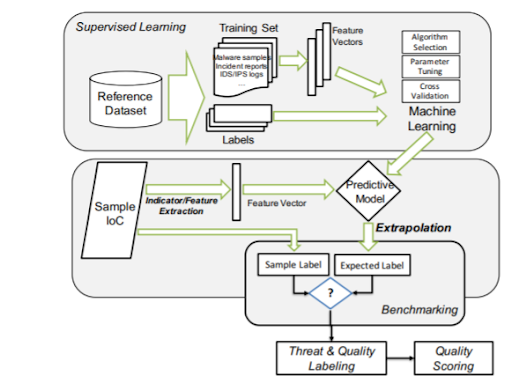
\includegraphics[width=1\linewidth]{Figures/co-relation}
    \caption{Co-relation process: Cyber news data}
    \label{fig:co-relation}
\end{figure}


\subsection{Analytics}
With the growing inflow of cyber newsfeed data 
and due to lack of cyber security professional performing analysis 
on the cyber newsfeed data, 
advanced analytics is gaming prominence 
and can be used in the consolidation process in order to simplify the mass of collected data \citep{dull2015cyberthreat}. 
In order to support the complexity of data structures 
of the cyber domain, 
the system should support, association, aggregation, composition and generalization \citep{brown2015cyber}. 
This domain is quite mature and literature suggest that 
big data architectures 
can be used to perform real-time network traffic processing, distributed messaging and scalable data storage. 
Then, the cyber professionals can focus on effective cyber threat intelligence analytics, 
rather than being hindered by data management, aggregation, reconciliation and formatting \citep{wheelus2016towards}. 

Automated and advanced Analytical capabilities of cyber threat intelligence platforms are mostly licensed and not available under open source distribution \citep{sauerwein2017threat}.

\section{Conclusion}
This concludes my literature work on the existing knowledge available for the current state of available artefacts mainly including people, processes and activities. This knowledge would be applied to the create the new artefact \enquote{Cybernewsfeed Technology}.


 
% Chapter 8

\chapter{Artefact Design} % Main chapter title

\label{Chapter8_artefact-design} % For referencing the chapter elsewhere, use \ref{Chapter7} 

\section{Introduction }
This chapter is about the designing of the prototype artefact Cybernewsfeed Technology using Design Science Research (DSR) 
\citep{hevner2010design}. 
The research method used for this specific piece of thesis work is Creative Process 
\citep{march1995design}  
as mentioned in chapter  
\ref{Chapter6_research-approach} 
(section \ref{Research Methodology: Design Science Research}). The artefact  has been termed as \enquote{Cybernewsfeed Technology} and this chapter provides a detailed explanation on the requirement and the final design of the \enquote{Cybernewsfeed Technology}.

\section{Requirement Specification}
%%% This file contains only a table.
%% this file is included into Chapter8

\begin{table}[htbp!]
   \setlength{\arrayrulewidth}{0.2mm}
    \setlength{\tabcolsep}{5pt}
    \renewcommand{\arraystretch}{1.0}

    \centering{}
 
    \caption{Requirements Modules}
    \label{table:Modules}
    
    \begin{tabularx}{0.92\linewidth}{|X| X|X|X|X|X|} 
    
%    |a|>{\columncolor[HTML]{FFFFFF}}C|C|C|
     \arrayrulecolor[HTML]{06000A}
        %% Table Body
       
        \hline
         \rowcolor[HTML]{BFCEED} \textbf{Modules-->}	&	\textbf{Collector}	&	\textbf{Processor}	&	\textbf{Analyser}	&	\textbf{Advisor}\\
        \hline
        \rowcolor[HTML]{EAEAFC}  Processes--> &	Collection &	Processing &	Analysis &	Advisory  \\
        \hline
       
       \rowcolor[HTML]{F6F6FB} Activities--> &	Collect, Source Management & Filtering, Contexting, Tagging, Data Manipulation and Output &	Provide Insight on tactics, severity and Impact &	Advice to Customer, Simple Writeup, Publishing                                  \\
       
        \hline
    \end{tabularx}

\end{table}











%\setlength{\arrayrulewidth}{0.5mm}
%\setlength{\tabcolsep}{10pt}
%\renewcommand{\arraystretch}{1.5}

%\newcolumntype{s}{>{\columncolor[HTML]{DDBDF7}} p{3cm}}


%\begin{tabular}{ |a | >{\columncolor[HTML]{5993C2}}c | l | b }

% \arrayrulecolor[HTML]{06000A}
% \hline
% \rowcolor[HTML]{5789F3} \multicolumn{4}{|c|}{High Level Modules = Collector} \\
% \hline
%  
%  \rowcolor[HTML]{BFCEED} Requirements: & What? & Why? & MoSCoW priority \\
% \hline
%
%Language Support	 & 	Support various languages.	 & 	To not miss intel in other languages	 & 	Must have	\\
% \hline
%Data Formats	 & 	Allow multiple data formats	 & 	To collect and process standard and recent formats	 & 	Should have	\\
% \hline
%Data Source types	 & 	Ingest from various sources	 & 	To cover broader sources of Intel	 & 	Must have	\\
% \hline
%Connection protocol	 & 	Support common protocols	 & 	To allow actual transfer To data	 & 	Must have	\\
 % 
%  \hline
% \end{tabular}
 



\subsection{Approach}

 To understand the requirements, my first step was to get familiar with the existing system, processes, activities and tools used in cyber newsfeeds publication. I took two simultaneous approaches: 1) searching knowledge in literature\footnote{According to literature review in chapter \ref{Chapter7_literature-review} } and 2) getting acquainted in a pragmatic way by working together with ON2IT team\footnote{Research and Development team, ON2IT Cybersecurity, The Nederlands}. The knowledge gained in the literature review was applied to the pragmatic approach where I was collaborating directly with the ON2IT team.
 
After understanding the processes and activities, I myself as an user\footnote{Role of Cyber Analyst for a certain period} started to work on the following four activities: 1) To manual scan of the cyber newsfeed sources,  2) To collect the cyber newsfeeds, 3) To analyse the newsfeeds and 4) To prepare advisory. Working with ON2IT team as an user helped me to understand the end-to-end flow of cyber newsfeeds publication.

Another step taken to enhance my understanding was simulating the existing system into a cloud environment. I choose a cloud environment to deploy, as it was easy to deploy and easy to collaborate as compared to my personal system. 
Simulation helped me to observe and understand the behaviour of the existing system used by the cyber experts. 
I also understood the way practitioners explore the sources to find relevant cyber newsfeed items. 


\subsection{Requirement Findings}
After two months of regular interactions with the ON2IT research and development team, it helped me to outline the requirements of the Artefact. 
Then the requirements were logically grouped based on the nature of activities as shown in FIGURE \ref{fig:modules}. I have termed
the list of such activities based groups as \enquote{High level Modules}. The name of modules classified as \enquote{High level Modules} are: 1) Collector, 2) Processor, 3) Analyser and 4) Advisor.  Based on the interactions from ON2IT team, I have elaborates on the requirements of each \enquote{High level Modules} in the following sections. 

\begin{figure}[ht]
    \centering
     
    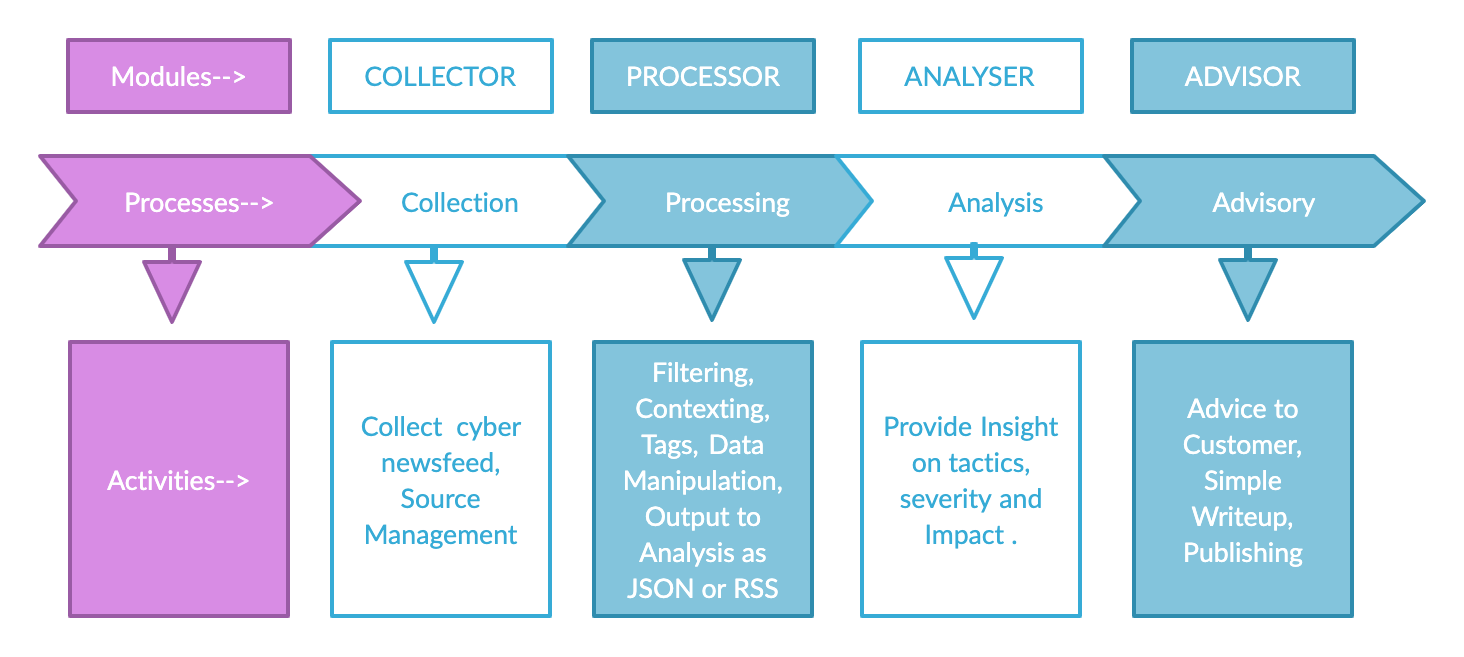
\includegraphics[width=1\linewidth]{Figures/Modules.png}
     
    \caption{Modules.
    \label{fig:modules}}
  
\end{figure}
\begin{enumerate}

    \item \textbf{Collector:}
    Collector helps to collect data from various cyber newsfeed sources and is an essential module required to proceed with the further activities of cyber newsfeed publication. 
    Collector enables to store the cyber newsfeed raw data in a repository. From this repository, the cyber newsfeed data can be assessed for further processing by the Processor module. 
    The  TABLE in \ref{table:collector-req} shows four essential requirements for the Collector module. 
    Along with requirement the reasoning is also mentioned with the priority.
%%% This file contains only a table.
%% this file is included into Chapter8

\begin{table}[htbp!]
   \setlength{\arrayrulewidth}{0.1mm}
    \setlength{\tabcolsep}{5pt}
    \renewcommand{\arraystretch}{1.0}

    \centering{}
 
    \caption{Requirements: Cyber data collection}
    \label{table:collector-req}
    
    \begin{tabularx}{0.92\linewidth}{|>{\columncolor[HTML]{ECB4E8}} p{2.2cm}|p{3.0cm}|p{4.4cm}|p{2cm}|} 
    
%    |a|>{\columncolor[HTML]{FFFFFF}}C|C|C|
     \arrayrulecolor[HTML]{06000A}
        %% Table Body
        \hline
        \rowcolor[HTML]{5789F3} 
        \multicolumn{4}{|c|}{High Level Modules = Collector} \\
        \hline
         \rowcolor[HTML]{BFCEED} Requirements: & What? & Why? & MoSCoW priority \\
        \hline
        Language Support	                    & 	
        Support various languages.	            & 	
        To not miss intel in other languages	& 	
        Must have	                            \\
        \hline
       
       
        Data Formats	                                    & 	
        Allow multiple data formats	                        & 	
        To collect and process standard and recent formats	& 	
        Should have	                                        \\
        \hline
       
        Data Source types	                & 	
        Ingest from various sources	        & 	
        To cover broader sources of Intel   & 	
        Must have	                        \\
       
        \hline
        Connection protocol	                & 	
        Support common protocols	        & 	
        To allow actual transfer To data	& 	
%|       \cellcolor[HTML]{AA0044}
        Must have	                        \\
       
        \hline
    \end{tabularx}

\end{table}











%\setlength{\arrayrulewidth}{0.5mm}
%\setlength{\tabcolsep}{10pt}
%\renewcommand{\arraystretch}{1.5}

%\newcolumntype{s}{>{\columncolor[HTML]{DDBDF7}} p{3cm}}


%\begin{tabular}{ |a | >{\columncolor[HTML]{5993C2}}c | l | b }

% \arrayrulecolor[HTML]{06000A}
% \hline
% \rowcolor[HTML]{5789F3} \multicolumn{4}{|c|}{High Level Modules = Collector} \\
% \hline
%  
%  \rowcolor[HTML]{BFCEED} Requirements: & What? & Why? & MoSCoW priority \\
% \hline
%
%Language Support	 & 	Support various languages.	 & 	To not miss intel in other languages	 & 	Must have	\\
% \hline
%Data Formats	 & 	Allow multiple data formats	 & 	To collect and process standard and recent formats	 & 	Should have	\\
% \hline
%Data Source types	 & 	Ingest from various sources	 & 	To cover broader sources of Intel	 & 	Must have	\\
% \hline
%Connection protocol	 & 	Support common protocols	 & 	To allow actual transfer To data	 & 	Must have	\\
 % 
%  \hline
% \end{tabular}
 

 %includes may not be nested

%% This file contains only a table.
%% this file is included into Chapter8

\begin{table}[htbp!]
   \setlength{\arrayrulewidth}{0.1mm}
    \setlength{\tabcolsep}{5pt}
    \renewcommand{\arraystretch}{1.0}

    \centering{}
 
    \caption{Requirements: Cyber data collection}
    \label{table:collector-req}
    
    \begin{tabularx}{0.92\linewidth}{|>{\columncolor[HTML]{ECB4E8}} p{2.2cm}|p{3.0cm}|p{4.4cm}|p{2cm}|} 
    
%    |a|>{\columncolor[HTML]{FFFFFF}}C|C|C|
     \arrayrulecolor[HTML]{06000A}
        %% Table Body
        \hline
        \rowcolor[HTML]{5789F3} 
        \multicolumn{4}{|c|}{High Level Modules = Collector} \\
        \hline
         \rowcolor[HTML]{BFCEED} Requirements: & What? & Why? & MoSCoW priority \\
        \hline
        Language Support	                    & 	
        Support various languages.	            & 	
        To not miss intel in other languages	& 	
        Must have	                            \\
        \hline
       
       
        Data Formats	                                    & 	
        Allow multiple data formats	                        & 	
        To collect and process standard and recent formats	& 	
        Should have	                                        \\
        \hline
       
        Data Source types	                & 	
        Ingest from various sources	        & 	
        To cover broader sources of Intel   & 	
        Must have	                        \\
       
        \hline
        Connection protocol	                & 	
        Support common protocols	        & 	
        To allow actual transfer To data	& 	
%|       \cellcolor[HTML]{AA0044}
        Must have	                        \\
       
        \hline
    \end{tabularx}

\end{table}











%\setlength{\arrayrulewidth}{0.5mm}
%\setlength{\tabcolsep}{10pt}
%\renewcommand{\arraystretch}{1.5}

%\newcolumntype{s}{>{\columncolor[HTML]{DDBDF7}} p{3cm}}


%\begin{tabular}{ |a | >{\columncolor[HTML]{5993C2}}c | l | b }

% \arrayrulecolor[HTML]{06000A}
% \hline
% \rowcolor[HTML]{5789F3} \multicolumn{4}{|c|}{High Level Modules = Collector} \\
% \hline
%  
%  \rowcolor[HTML]{BFCEED} Requirements: & What? & Why? & MoSCoW priority \\
% \hline
%
%Language Support	 & 	Support various languages.	 & 	To not miss intel in other languages	 & 	Must have	\\
% \hline
%Data Formats	 & 	Allow multiple data formats	 & 	To collect and process standard and recent formats	 & 	Should have	\\
% \hline
%Data Source types	 & 	Ingest from various sources	 & 	To cover broader sources of Intel	 & 	Must have	\\
% \hline
%Connection protocol	 & 	Support common protocols	 & 	To allow actual transfer To data	 & 	Must have	\\
 % 
%  \hline
% \end{tabular}
 



    \item \textbf{Processor:}
     Processor module would be responsible for cyber newsfeed data filtering, manipulation and tagging.
     The data filtering manipulation and tagging methods should support filtration, manipulation and tagging based on the configurable parameters. 
     The Processor module must verify the content of the configured tags and must add a tag to the cyber newsfeed data based on the input parameters. 
     The input parameters could be stakeholders specific or an organisation specific.
     The TABLE \ref{table:processor-req} contains the list of requirements for the Processor module.
    
%% This file contains only a table.
%% this file is included into Chapter8

\begin{table}[htbp!]
   \setlength{\arrayrulewidth}{0.1mm}
    \setlength{\tabcolsep}{5pt}
    \renewcommand{\arraystretch}{1.0}

    \centering{}
 
    \caption{Requirements: Cyber data processing}
    \label{table:processor-req}
    
    \begin{tabularx}{0.92\linewidth}{|>{\columncolor[HTML]{ECB4E8}} p{2.2cm}|p{3.0cm}|p{4.4cm}|p{2cm}|} 
    
%    |a|>{\columncolor[HTML]{FFFFFF}}C|C|C|
     \arrayrulecolor[HTML]{06000A}
        %% Table Body
        \hline
        \rowcolor[HTML]{5789F3} 
        \multicolumn{4}{|c|}{High Level Module = Processor} \\
        \hline
         \rowcolor[HTML]{BFCEED} Requirements: & What? & Why? & MoSCoW priority \\
        \hline
      Data structuring	 & 	Data mappings and Data format conversion	 & 	To ensure a common data format To enable further processing	 & 	Should have	\\
       \hline
Contextualiz-ation	 & 	Possible to set context	 & 	To convert raw intel To specific intel	 & 	Must have	\\
       
        \hline
Data Filtering	 & 	Be able to filter data 	 & 	Based on adjustable parameters	 & 	Must have	\\
       
        \hline
    \end{tabularx}

\end{table}











%\setlength{\arrayrulewidth}{0.5mm}
%\setlength{\tabcolsep}{10pt}
%\renewcommand{\arraystretch}{1.5}

%\newcolumntype{s}{>{\columncolor[HTML]{DDBDF7}} p{3cm}}


%\begin{tabular}{ |a | >{\columncolor[HTML]{5993C2}}c | l | b }

% \arrayrulecolor[HTML]{06000A}
% \hline
% \rowcolor[HTML]{5789F3} \multicolumn{4}{|c|}{High Level Modules = Collector} \\
% \hline
%  
%  \rowcolor[HTML]{BFCEED} Requirements: & What? & Why? & MoSCoW priority \\
% \hline
%
%Language Support	 & 	Support various languages.	 & 	To not miss intel in other languages	 & 	Must have	\\
% \hline
%Data Formats	 & 	Allow multiple data formats	 & 	To collect and process standard and recent formats	 & 	Should have	\\
% \hline
%Data Source types	 & 	Ingest from various sources	 & 	To cover broader sources of Intel	 & 	Must have	\\
% \hline
%Connection protocol	 & 	Support common protocols	 & 	To allow actual transfer To data	 & 	Must have	\\
 % 
%  \hline
% \end{tabular}
 


    
%%% This file contains only a table.
%% this file is included into Chapter8

\begin{table}[htbp!]
   \setlength{\arrayrulewidth}{0.1mm}
    \setlength{\tabcolsep}{5pt}
    \renewcommand{\arraystretch}{1.0}

    \centering{}
 
    \caption{Requirements: Cyber data collection}
    \label{table:collector-req}
    
    \begin{tabularx}{0.92\linewidth}{|>{\columncolor[HTML]{ECB4E8}} p{2.2cm}|p{3.0cm}|p{4.4cm}|p{2cm}|} 
    
%    |a|>{\columncolor[HTML]{FFFFFF}}C|C|C|
     \arrayrulecolor[HTML]{06000A}
        %% Table Body
        \hline
        \rowcolor[HTML]{5789F3} 
        \multicolumn{4}{|c|}{High Level Modules = Collector} \\
        \hline
         \rowcolor[HTML]{BFCEED} Requirements: & What? & Why? & MoSCoW priority \\
        \hline
        Language Support	                    & 	
        Support various languages.	            & 	
        To not miss intel in other languages	& 	
        Must have	                            \\
        \hline
       
       
        Data Formats	                                    & 	
        Allow multiple data formats	                        & 	
        To collect and process standard and recent formats	& 	
        Should have	                                        \\
        \hline
       
        Data Source types	                & 	
        Ingest from various sources	        & 	
        To cover broader sources of Intel   & 	
        Must have	                        \\
       
        \hline
        Connection protocol	                & 	
        Support common protocols	        & 	
        To allow actual transfer To data	& 	
%|       \cellcolor[HTML]{AA0044}
        Must have	                        \\
       
        \hline
    \end{tabularx}

\end{table}











%\setlength{\arrayrulewidth}{0.5mm}
%\setlength{\tabcolsep}{10pt}
%\renewcommand{\arraystretch}{1.5}

%\newcolumntype{s}{>{\columncolor[HTML]{DDBDF7}} p{3cm}}


%\begin{tabular}{ |a | >{\columncolor[HTML]{5993C2}}c | l | b }

% \arrayrulecolor[HTML]{06000A}
% \hline
% \rowcolor[HTML]{5789F3} \multicolumn{4}{|c|}{High Level Modules = Collector} \\
% \hline
%  
%  \rowcolor[HTML]{BFCEED} Requirements: & What? & Why? & MoSCoW priority \\
% \hline
%
%Language Support	 & 	Support various languages.	 & 	To not miss intel in other languages	 & 	Must have	\\
% \hline
%Data Formats	 & 	Allow multiple data formats	 & 	To collect and process standard and recent formats	 & 	Should have	\\
% \hline
%Data Source types	 & 	Ingest from various sources	 & 	To cover broader sources of Intel	 & 	Must have	\\
% \hline
%Connection protocol	 & 	Support common protocols	 & 	To allow actual transfer To data	 & 	Must have	\\
 % 
%  \hline
% \end{tabular}
 

 %includes may not be nested

    \item \textbf{Analyzer:}
    The Analyser module is required for correlation and analysis on the cyber newsfeed data processed by the Processor module. 
    The correlation and analysis activities would be done manually by the cyber experts in the first version of the artefact. The artefact should provide a GUI to conduct analysis and correlation activities. The detailed requirements of this module is in TABLE \ref{table:analyzer-req}
    %% This file contains only a table.
%% this file is included into Chapter8

\begin{table}[htbp!]
   \setlength{\arrayrulewidth}{0.1mm}
    \setlength{\tabcolsep}{5pt}
    \renewcommand{\arraystretch}{1.0}

    \centering{}
 
    \caption{Requirements: Cyber data analysis}
    \label{table:analyzer-req}
    
    \begin{tabularx}{0.92\linewidth}{|>{\columncolor[HTML]{ECB4E8}} p{2.2cm}|p{3.0cm}|p{4.4cm}|p{2cm}|} 
    
%    |a|>{\columncolor[HTML]{FFFFFF}}C|C|C|
     \arrayrulecolor[HTML]{06000A}
        %% Table Body
        \hline
        \rowcolor[HTML]{5789F3} 
        \multicolumn{4}{|c|}{High Level Module = Analyser} \\
        \hline
         \rowcolor[HTML]{BFCEED} Requirements: & What? & Why? & MoSCoW priority \\
        \hline
     Co-relation	 & 	Group similar Intel	 & 	To reduce duplicity and improve granularity	 & 	Should have	\\
      \hline
Analysis	 & 	Provide insights on tactics, severity and impact	 & 	To make the cyber intel actionable	 & 	Must have	\\
       
        \hline
    \end{tabularx}

\end{table}











%\setlength{\arrayrulewidth}{0.5mm}
%\setlength{\tabcolsep}{10pt}
%\renewcommand{\arraystretch}{1.5}

%\newcolumntype{s}{>{\columncolor[HTML]{DDBDF7}} p{3cm}}


%\begin{tabular}{ |a | >{\columncolor[HTML]{5993C2}}c | l | b }

% \arrayrulecolor[HTML]{06000A}
% \hline
% \rowcolor[HTML]{5789F3} \multicolumn{4}{|c|}{High Level Modules = Collector} \\
% \hline
%  
%  \rowcolor[HTML]{BFCEED} Requirements: & What? & Why? & MoSCoW priority \\
% \hline
%
%Language Support	 & 	Support various languages.	 & 	To not miss intel in other languages	 & 	Must have	\\
% \hline
%Data Formats	 & 	Allow multiple data formats	 & 	To collect and process standard and recent formats	 & 	Should have	\\
% \hline
%Data Source types	 & 	Ingest from various sources	 & 	To cover broader sources of Intel	 & 	Must have	\\
% \hline
%Connection protocol	 & 	Support common protocols	 & 	To allow actual transfer To data	 & 	Must have	\\
 % 
%  \hline
% \end{tabular}
 

.

    \item \textbf{Advisory:}
    The requirement for this module is help cyber analyst in drafting a nice list of cyber newsfeed advisory. The Advisory module should ship the outbound communication to the stakeholders, via a certain communication channel. If possible, the Advisory module should also collect the feedback from users. The exact requirements of the Advisory module are listed in the %% This file contains only a table.
%% this file is included into Chapter8

\begin{table}[htbp!]
   \setlength{\arrayrulewidth}{0.1mm}
    \setlength{\tabcolsep}{5pt}
    \renewcommand{\arraystretch}{1.0}

    \centering{}
 
    \caption{Requirements: Cyber Intel advisory}
    \label{table:advisory-req}
    
    \begin{tabularx}{0.92\linewidth}{|>{\columncolor[HTML]{ECB4E8}} p{2.2cm}|p{3.0cm}|p{4.4cm}|p{2cm}|} 
    
%    |a|>{\columncolor[HTML]{FFFFFF}}C|C|C|
     \arrayrulecolor[HTML]{06000A}
        %% Table Body
        \hline
        \rowcolor[HTML]{5789F3} 
        \multicolumn{4}{|c|}{High Level Module = Advisory} \\
        \hline
         \rowcolor[HTML]{BFCEED} Requirements: & What? & Why? & MoSCoW priority \\
        \hline
     Writing custom intel	 & 	Allow to write a new content for cyber news feed	 & 	To ensure that analyst can use his knowledge for providing details on cyber news	 & 	Must have	\\
     \hline
Template Designing	 & 	Make design template for writing cyber intel and advisories	 & 	To allow flexibility in presentation of cyber Intel To further streams	 & 	Should have	\\
\hline
Feedback Collection	 & 	Collect internal and external user feedback	 & 	To check the quality and if the news is actionable	 & 	Could have	\\
\hline
Outbound Communication	 & 	Deliver Cyber news feed to users	 & 	To ensure cyber intel with advisory reach To destination	 & 	Must have	\\
       
        \hline
    \end{tabularx}

\end{table}











%\setlength{\arrayrulewidth}{0.5mm}
%\setlength{\tabcolsep}{10pt}
%\renewcommand{\arraystretch}{1.5}

%\newcolumntype{s}{>{\columncolor[HTML]{DDBDF7}} p{3cm}}


%\begin{tabular}{ |a | >{\columncolor[HTML]{5993C2}}c | l | b }

% \arrayrulecolor[HTML]{06000A}
% \hline
% \rowcolor[HTML]{5789F3} \multicolumn{4}{|c|}{High Level Modules = Collector} \\
% \hline
%  
%  \rowcolor[HTML]{BFCEED} Requirements: & What? & Why? & MoSCoW priority \\
% \hline
%
%Language Support	 & 	Support various languages.	 & 	To not miss intel in other languages	 & 	Must have	\\
% \hline
%Data Formats	 & 	Allow multiple data formats	 & 	To collect and process standard and recent formats	 & 	Should have	\\
% \hline
%Data Source types	 & 	Ingest from various sources	 & 	To cover broader sources of Intel	 & 	Must have	\\
% \hline
%Connection protocol	 & 	Support common protocols	 & 	To allow actual transfer To data	 & 	Must have	\\
 % 
%  \hline
% \end{tabular}
 

 TABLE \ref{table:advisory-req}.
   \FloatBarrier
\end{enumerate}

\subsection{Contribution to Stakeholder Goals}
In this section I have assumed the needs of cyber newsfeed intel for the stakeholders according to the literature. The stakeholders are positioned at different functional layers and are broadly classified into three levels 1) Strategic 2) Tactical and 3) Operational level. Stakeholders
\citep{farnham2013tools} are the users of cyber newsfeed intel and are collectively responsible for securing their organisational IT infrastructures. 

The board, which works at strategic level is interested in legal implications of a security breach. 
The tactical level is responsible for ensuring the fulfilment of strategic needs with the help of operational levels. 
For Instance, the analysis of loss and listing potential vulnerable assets would be scope of tactical level. 
The operational layer is responsible for taking steps to stop actual security incidents. 
For example, applying a secure patch. 

The stakeholders needs relevant and actionable intelligence rather than raw information
\citep{tounsi2018survey}.  
Following are certain characteristics required in the cyber newsfeed items to become an actionable cyber newsfeed. 

\begin{itemize}
    \item \textbf{Timely:} For effective threat intelligence time plays a critical role. 
    Intelligence ought to be quickly conveyed with insignificant idleness. 
    
    \item \textbf{Relevant:} 
    Threat intelligence needs to apply to the related environment. 
    \item  \textbf{Accurate:} 
    To be able to take more reasonable and effective measurements against attacks more accurate intelligence is necessary. Therefore, the information which is provided by threat intelligence should be correct, complete, and explicit. 
    
    \item \textbf{Specific:} 
    More detailed and more specific threat intelligence can allow defenders to choose suitable countermeasures.
    
    \item \textbf{Actionable}: 
    Actions are needed to be identified by threat intelligence to ensure necessary data for the response against threats.

\end{itemize}


The mapping between the concerned cyber newsfeed type and the stakeholders is shown in the FIGURE \ref{fig:stakeholder-problem}.

\begin{figure}[ht]
    \centering
     
    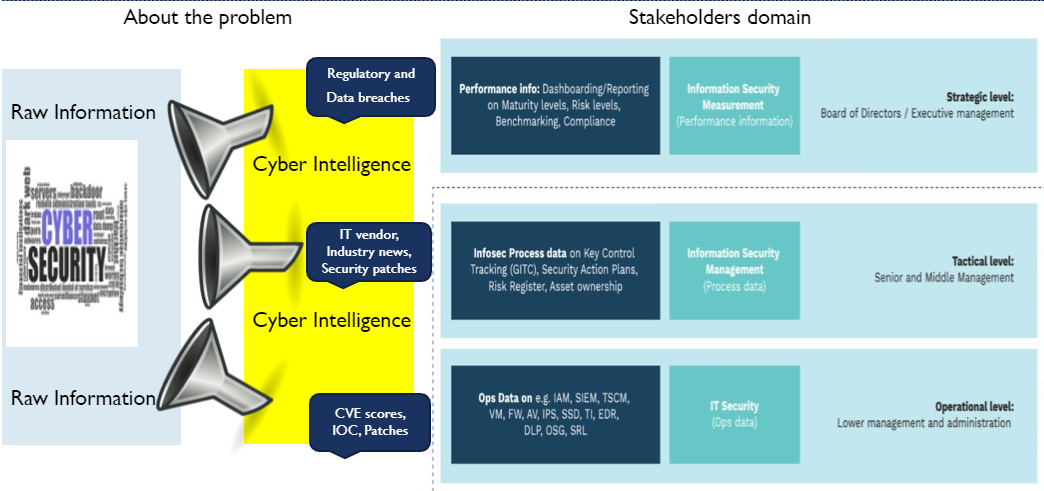
\includegraphics[width=1\linewidth]{Figures/stakeholder-problem}
     
    \caption{Stakeholders: Volumetric Problems at Three levels.
    \label{fig:stakeholder-problem}}
  
\end{figure}

According to ON2IT team, the cyber newsfeed intelligence can be analysed, classified and Tagged into one of the the levels: 1) Strategic, 2) Tactical and 3) Operational to make it interceptable at the stakeholders end. 



\begin{table}[hbt!]
    \caption{Cyber Information needs per level}
    \label{tab:stakeholder-news}
    \centering
    \resizebox{0.75\textwidth}{!}{%
        \begin{tabular}{|l|l|}
        \toprule
            \textbf{Indented news Level} & 
            \textbf{Cyber newsfeed type} \\
            \midrule
            Strategic & Regulatory News	\\
            Strategic & Data breaches - sector	\\
            Strategic/Tactical & Guidelines from community bodies (NCSC)\\
            Strategic/Tactical & Industry news\\
            Tactical/Operational & Security vendor news (new releases patches)\\
            Tactical & Market indicators and reports\\
            Operational & Important updates from tech vendors	\\
            Operational & CVE scores , Advisory, IOC , Impact	\\
            \bottomrule
        \end{tabular}
    }
\end{table}

\subsection{Available artefact}
The available artefact in practice was Taranis\footnote{About Taranis \url{https://github.com/NCSC-NL/taranis3/wiki}} at ON2IT. Other tools mentioned in the list \ref{tab:tip-list} are according to the literature. 
Taranis is used for collection and source management, 
further the filtering and selection of cyber newsfeed is a manual process. 
Although Taranis support the feature of pushing publication after advisory but it is barely used to perform such activities. 
The main reason is partial ingestion of cyber newsfeeds for any particular topic and complex data models in the Taranis database. 

There are list \ref{tab:tip-list} of tools  including Taranis  that only support parts of the functionality like collecting the cyber newsfeed data but they do not fulfill the  needs of customised data processing and relevance tagging,  therefore a new artefact was needed.

\section{New artefact prototype}\label{New artefact prototype design}
This section covers in detail about the newly created artefact:  
1) Prototype to filter contextual cyber Intelligence, perform automatic relevance tagging and perform analysis for automated risk determination and advisory and 
2)  Prototype on accessing the data source quality to keep data sources sanitized

\subsection{Prototype for, filtering contextual feeds, perform automatic tagging and analysis of risk determination and advisory.}

\subsubsection{Introduction}
This section describes the approach and work done to build the artefact. 
In the subsequent sections, there is logical segregation done based on the activities done to deliver the artefact.
It also includes the list of modules required to build the artefact where 
each artefact module is then explained in detail. 


\begin{table}
    \caption{Assessment Parameters for tool selection}
    \label{table: assessment-parameters}
    \centering{}
   \resizebox{0.75\textwidth}{!}{
    \begin{tabular}{|>{\columncolor[HTML]{ECB4E8}}l|l|}
    \toprule
      \rowcolor[HTML]{BFCEED} 
    
    \textbf{Assessment Parameters} & \textbf{Focus}\\
    \midrule
    Distribution & Open Source\\
    Application Support Forum  Available? & Ease of trouble shoot\\
    Application Active Since years & Old and stable\\
    Application's Last Issue resolved date & Most recent is better\\
    Functional Features &	More is better\\
    Database and GUI & User Friendly\\
   \bottomrule
 
    \end{tabular}
}
\end{table}

\subsubsection{Approach to build artefact}
After the process of requirement elicitation, the artefact requirements were clear and I started evaluating available threat intelligence tools based on the assessment parameters listed in table \ref{table: assessment-parameters} for the required functionality and priority. 
An ideal threat intelligence tool should provide Collector, Processor, Analyser and Advisory modules. Finding everything in one tool which is readily available in one threat intelligence tool was not possible. 
Out of 17 listed tool in \ref{tab:tip-list}, four were shortlisted as listed in table \ref{tab:four-tool}.


\begin{table}
    \caption{Shortlisted tools for cybernewfeed technology}
    \label{tab:four-tool}
    \centering{}
   \resizebox{\textwidth}{!}{
    \begin{tabular}{|>{\columncolor[HTML]{ECB4E8}}l|l|}
    \toprule
      \rowcolor[HTML]{BFCEED} 
    
    \textbf{Shortlisted Applications} & \textbf{Brief Overview}\\
    \midrule
   
FreshRSS & 
Good choice only for Collection \\
MISP: Open-source threat intelligence platform &
Used to store, share and collaborate on cyber security indicators\\
CRITs: Collaborative Research Into Threats &
CISCO will stop Grant in 2020\\
Collection Intel Framework &
Combine with machine learning to produce unified threat feeds\\

   \bottomrule
 
    \end{tabular}
}
\end{table}




We chose Fressrss from existing lists of vendors which provide newsfeed collection as open source for Collector process. This module will collect and store cyber newsfeed information in a central repository. On the top of Collector module, we  build Processor, Analyser and Advisory. We developed the functionality of data filtering, text manipulation, relevance tagging on the information stored in the central repository. We have used AWS cloud to build, deploy and run the solution because of the two reasons. 1) The cloud usage charges could be paid on hourly basis and 2) I am much familiar with AWS cloud then other cloud providers.

\subsection{Argumentation}
This section explains the logic and rationale used to choose any specific processes, activities or tools for the purpose of building the artefact. Let’s see in detail.

At general level, we had six parameters for overall evaluation of a threat intel tool. 
Those parameters are listed below with the focus area. 
We were looking for a stable
\citep{THE-BIT-DEPTH-BLOG} open source tool\footnote{Refer to defination of open source software according to Wikipedia \url{https://en.wikipedia.org/wiki/Open-source_software}} with maximum functionality and is easy to operate. 
The preference to select a stable open source tools was to save the time by reusing a stable tool and saving cost by using open source.

There were total 23 tools evaluated and four shortlisted to look into more detail. Out of these four tools, FressRss was selected because of it’s primarily capability to collect newsfeed information from different sources in a central repository and its simplicity of deployment and control on information collected. As the FreshRSS is PHP based application with MySQL as database, to process information further, it was easy to build custom modules on the top of the central repository.  

For Processor module, we developed our own configurable system because the rule required to filter, contextualize, tag and categorize is specific to stakeholder needs and does not comes with any available open source tool. Similarly, Analyser and Advisory modules are human intensive and require certain process set-up specific to the stakeholder need. Both cyber analysis and editorial tasks requires human intervention to provide essential insights. 

\subsection{Artefact and Artefact breakdown }\label{Artefact and Artefact breakdown}
\begin{figure}[ht]
    \centering
    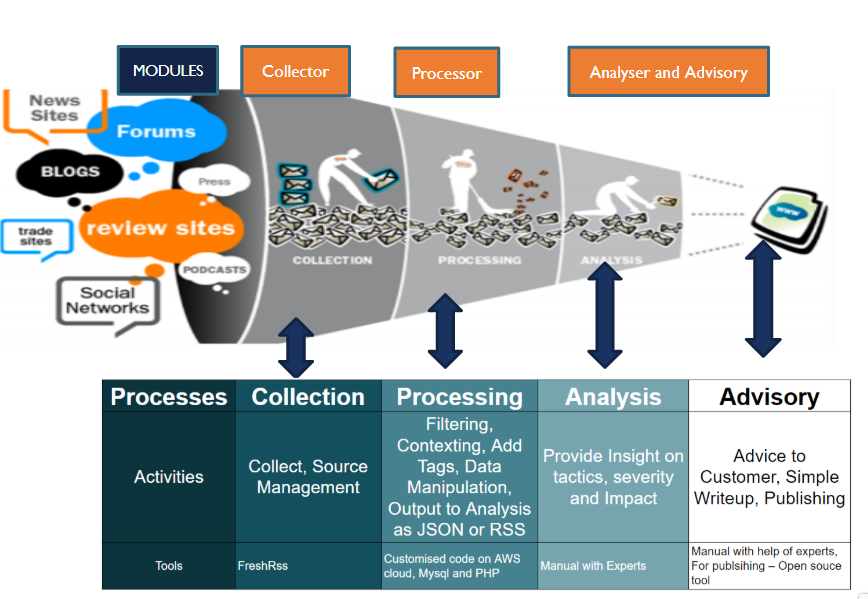
\includegraphics[width=1\linewidth,height=0.5\textwidth]{Figures/solution-breakup.PNG}
    \caption{Artefact: At a glance}
    \label{fig:solution-breakup}
\end{figure}

\subsubsection{Collector Module}
The model of the Collector module in the artefact has been depicted in FIGURE \ref{fig:collector}.
The Collector module is designed to collect cyber newsfeed from different web based data sources and source management.   
 For example, a data source \enquote{feed:\url{https://www.darkreading.com/rss_simple.asp?f_n=644&f_ln=Attacks/Breaches} }can be added as a source in the Collector module. By doing data source management, an user can add, 
remove and update the list of data sources in the Collector module.
The Collector module is  the core of the \enquote{Cybernewsfeed Technology} because this module collects and stores information for further processing. Using the Collector module, an user can collect cyber newsfeeds in other languages.
It can also collect data in real time mode as well as in batch mode as shown in FIGURE \ref{ref:collector-batch}. 
In case the Collector module has not run in last few days, the user can use batch mode to collect the backlog data. 

We have used open source tool FressRSS and installed it on AWS cloud for simulating the Collector module.

\begin{figure}[ht]
    \centering
    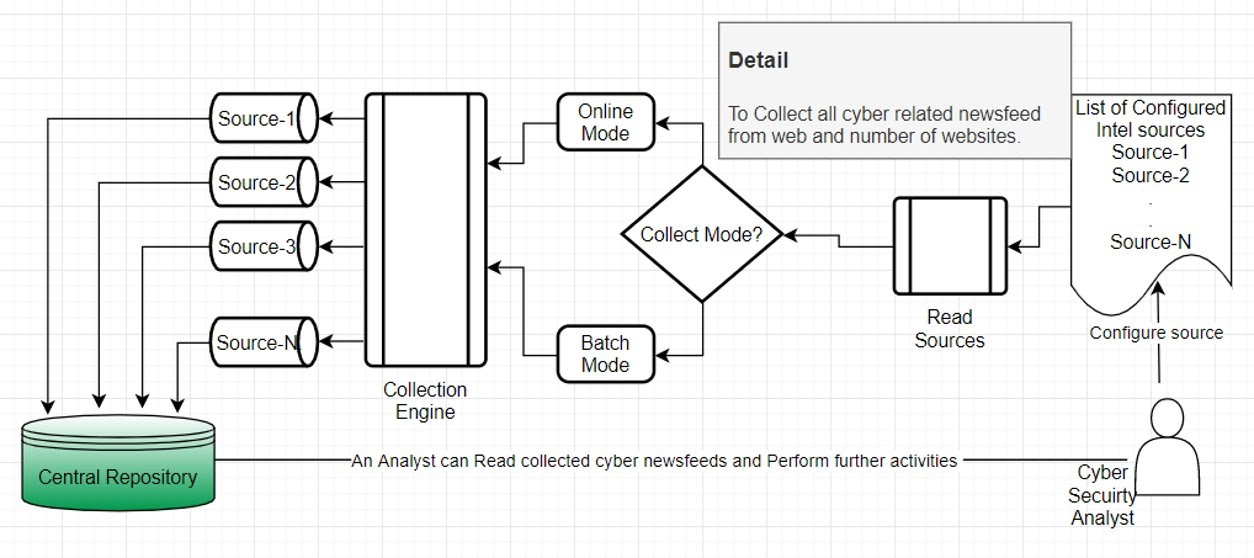
\includegraphics[width=1\linewidth]{Figures/collector.png}
    \caption{Collection Module Design}
    \label{fig:collector}
\end{figure}


\begin{figure}[ht]
\centering
    \fbox{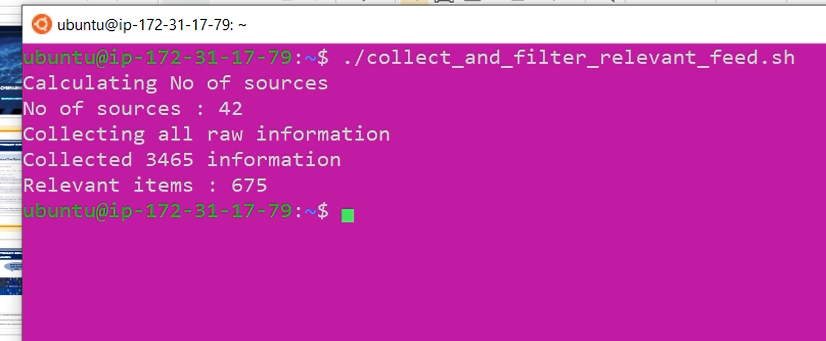
\includegraphics[width=.75\linewidth]{Figures/Collector-Demo.PNG}}
    \caption{Screenshot of the artefact: FreshRSS in Batch collection }
    \label{ref:collector-batch}
\end{figure}

In the FIGURE \ref{ref:collector-batch}, 
we see that the script invoked the batch job to collect the cyber newsfeed from 42 sources, 
it scanned and collected 3465 information and highlighted 675 relevant items.

\subsubsection{Processor Module}
The Processor module is at the heart of this cybernewsfeed technology and the model of the Processor module in the artefact has been depicted in FIGURE \ref{fig:processor}. 
\begin{figure}[ht]
    \centering
    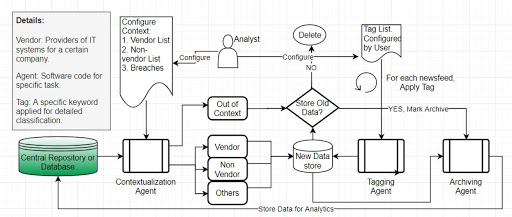
\includegraphics[width=1\linewidth]{Figures/processor.png}
    \caption{Processor Module Design}
    \label{fig:processor}
\end{figure}
 \FloatBarrier
In the Processor module, the first step is to configure the organisation-specific context by using TAGs. To configure the organisation-specific context, the Processor module needs the list of context and tags from the organisation-specific stakeholders.  A cyber security analyst can configure the organisational-specific context by use of the keywords, 
see FIGURE \ref{fig:tag} for tag management and FIGURE \ref{fig:Configured-tags} for the list of already configured tags. In this demo we have considered Vendor and Non-Vendor aspects of the context for ON2IT and TAGs like (Relevant Vendors: Cisco, Palo Alto, etc and Less relevant Vendors for ON2IT: Zoom, etc). The configured keywords in  the Processor module filters the organisation-specific cyber newsfeed according to the code mentioned in \ref{filter-context} in Appendix \ref{AppendixChapter8}.

\begin{figure}[ht]
    \centering
    \fbox{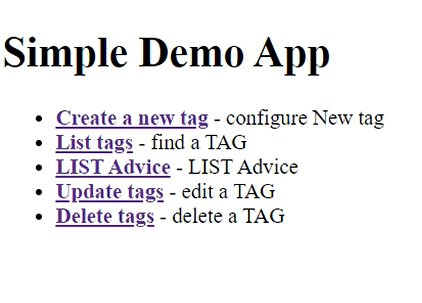
\includegraphics[width=.5\linewidth]{Figures/tag.PNG}}
    \caption{Screenshot of the artefact: Demo for TAG management}
    \label{fig:tag}
\end{figure}
 \FloatBarrier
    At the second level of processing in the Processor module, a tagging agent (software) 
tags the  cyber newsfeed with specific tags at more granular level to classify 
the news into detailed contexts, 
as specified in FIGURE \ref{tab:stakeholder-news} using code in \ref{tag-addtag} in Appendix \ref{AppendixChapter8}.

\begin{figure}[ht]
    \centering
    \fbox{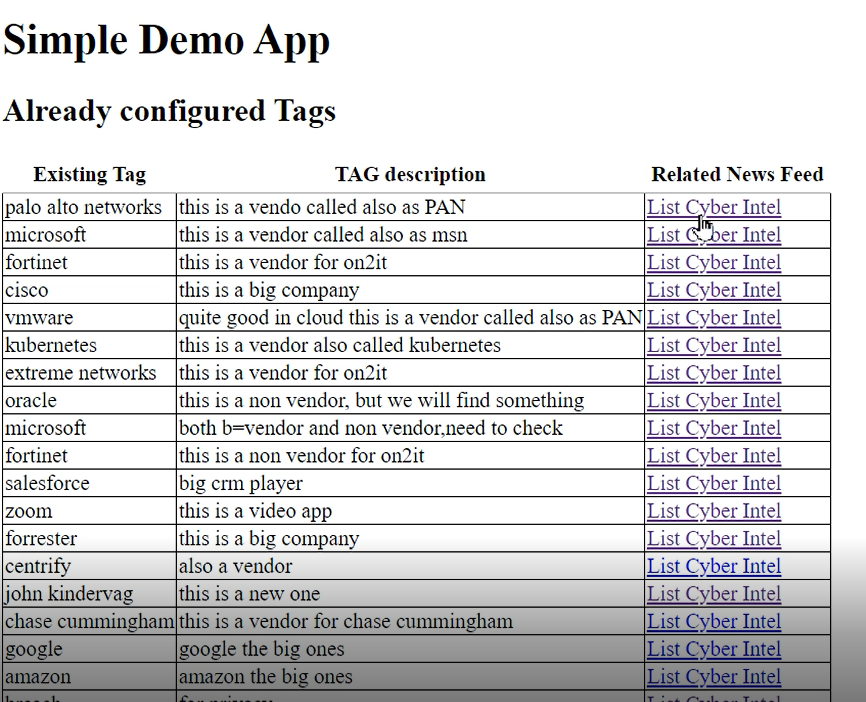
\includegraphics[width=1\linewidth]{Figures/Configured-tags.PNG}}
    \caption{Screenshot of the artefact: List of TAGs}
    \label{fig:Configured-tags}
\end{figure}
 \FloatBarrier

After tagging and filteration steps, 
our newsfeed is ready for correlation and analysis  work. The cyber newsfeeds which are not relevant are achieved and are not considered for the further processing.
We have used custom MySQL database, PHP frontend, Apache webserver and custom SQL scripts on AWS cloud to do the information processing.



In FIGURE \ref{fig:processor-rss}, we see the output as a RSS feed which can be used by a Cyber analyst for further analysis. The filter logic is mentioned in section \ref{rss-send} of Appendix \ref{AppendixChapter8}.

\begin{figure}[ht]
    \centering
   \fbox{ 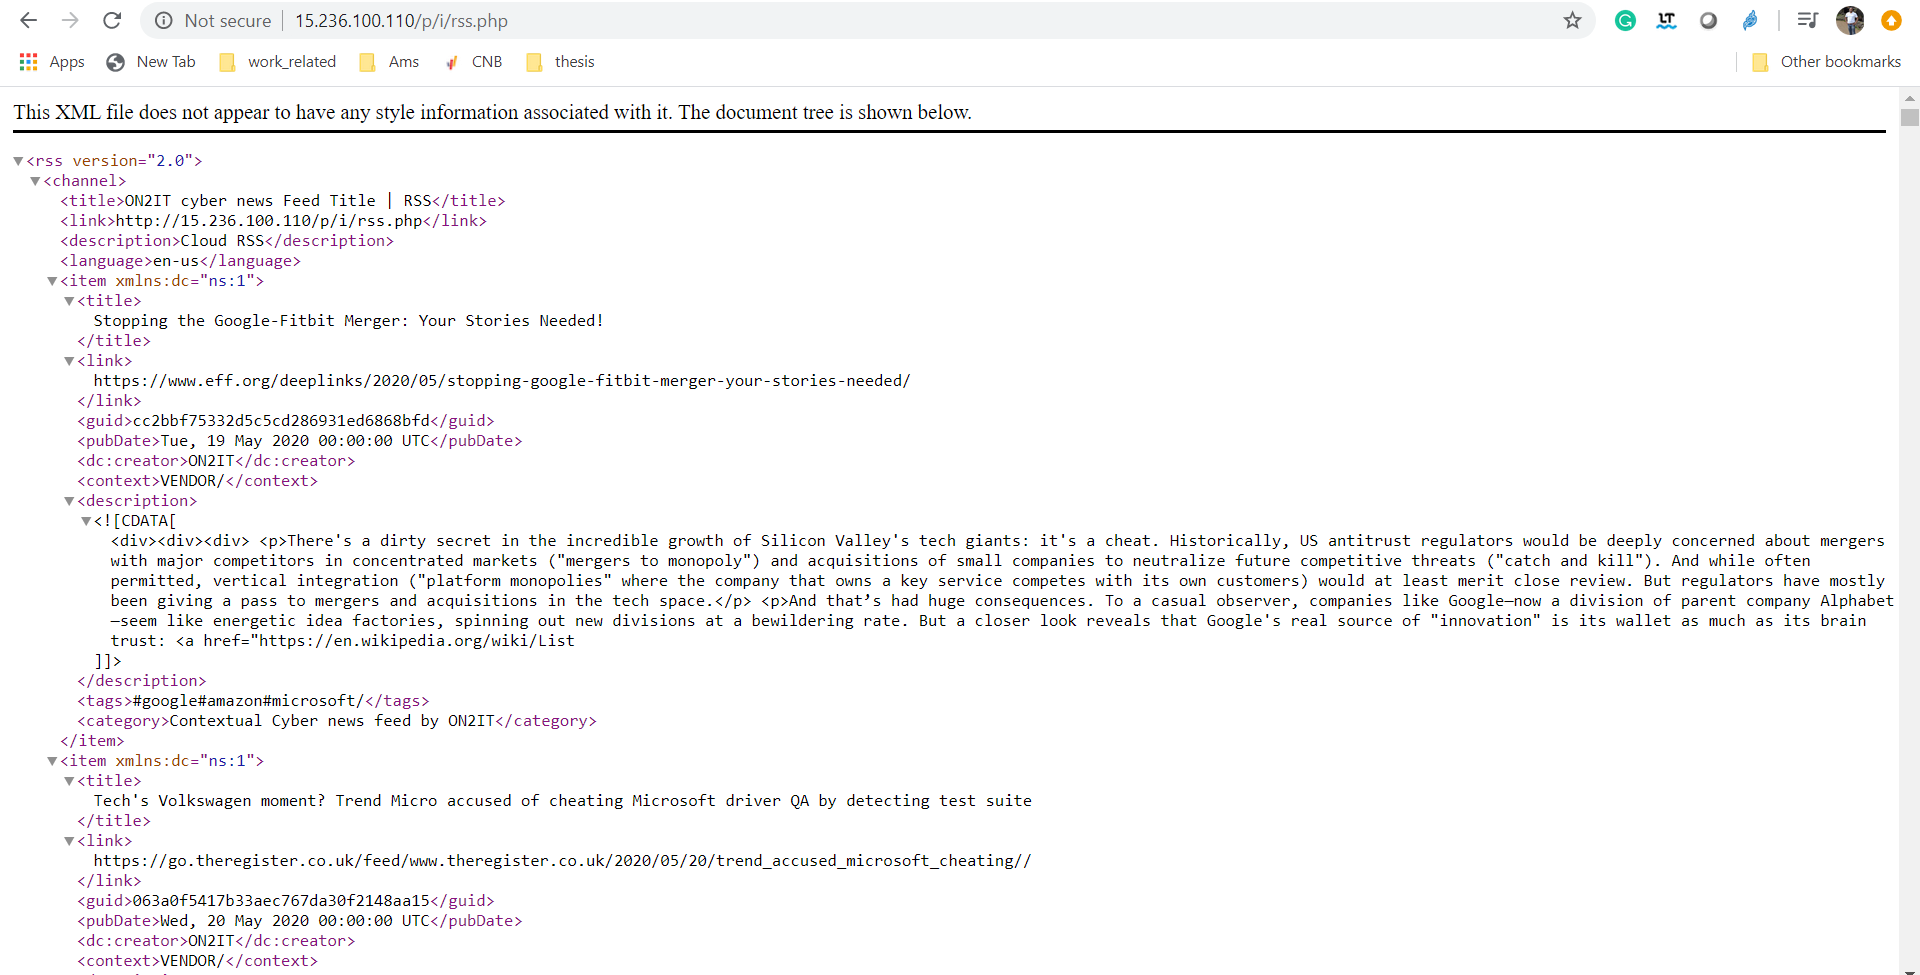
\includegraphics[width=1\linewidth]{Figures/processor-rss-output.png}}
    \caption{Screenshot of the artefact: Processor Module RSS output}
    \label{fig:processor-rss}
\end{figure}
 \FloatBarrier
\subsubsection{Analyser \& Advisory Module}
Despite having different functionality of the Analyser \& Advisory Module, I have merged the two functionalities 1) Analyser and 2) Advisory into a single module. This is done because both the modules are human dependent and it is assumed that the cyber analysts will do the Analysis and Advisory activities using the same GUI. The Analyser \& Advisory module is a mix of automatic and manual work as depicted in  FIGURE \ref{fig:analyser-advisor}

\begin{figure}[ht]
    \centering
    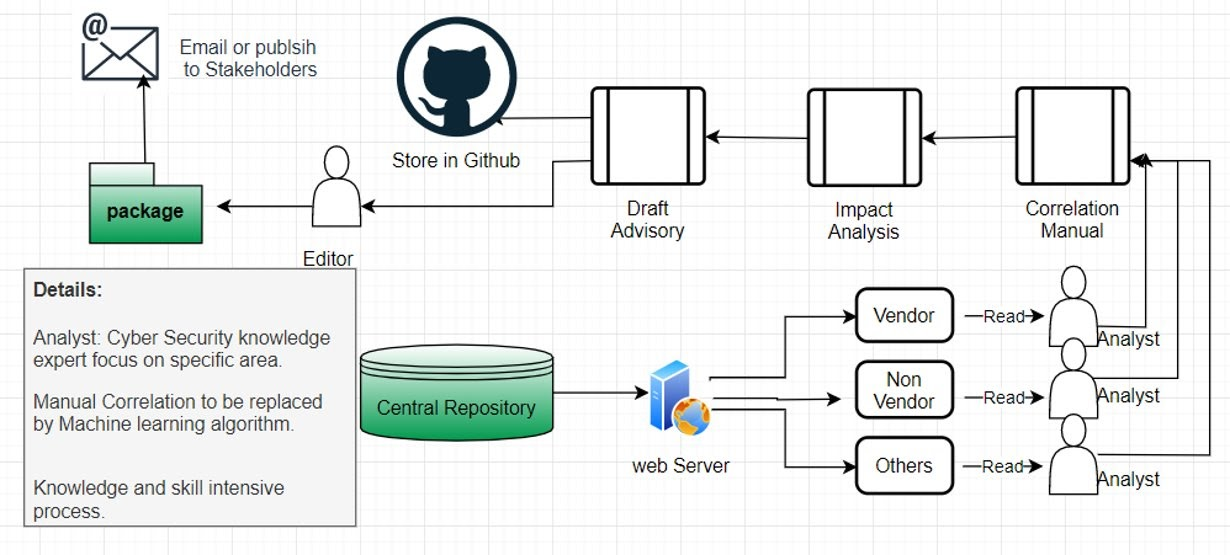
\includegraphics[width=1\linewidth]{Figures/analyser-advisor.png}
    \caption{Analyser \& Advisory Module design}
    \label{fig:analyser-advisor}
\end{figure}
 \FloatBarrier
 
 As shown in FIGURE \ref{fig:tag-intel}, 
 the cyber analysts can use the web interface of Analyser \& Advisory module 
 to find the related cyber newsfeed info.
 The cyber analysts can refer to the related cyber newsfeed data 
 and after doing their research can add advisory for the organisation-specific cyber newsfeed topic 
 as depicted in FIGURE 
 \ref{fig:add-advisory}. 
 
\begin{figure}[ht]
    \centering
    \fbox{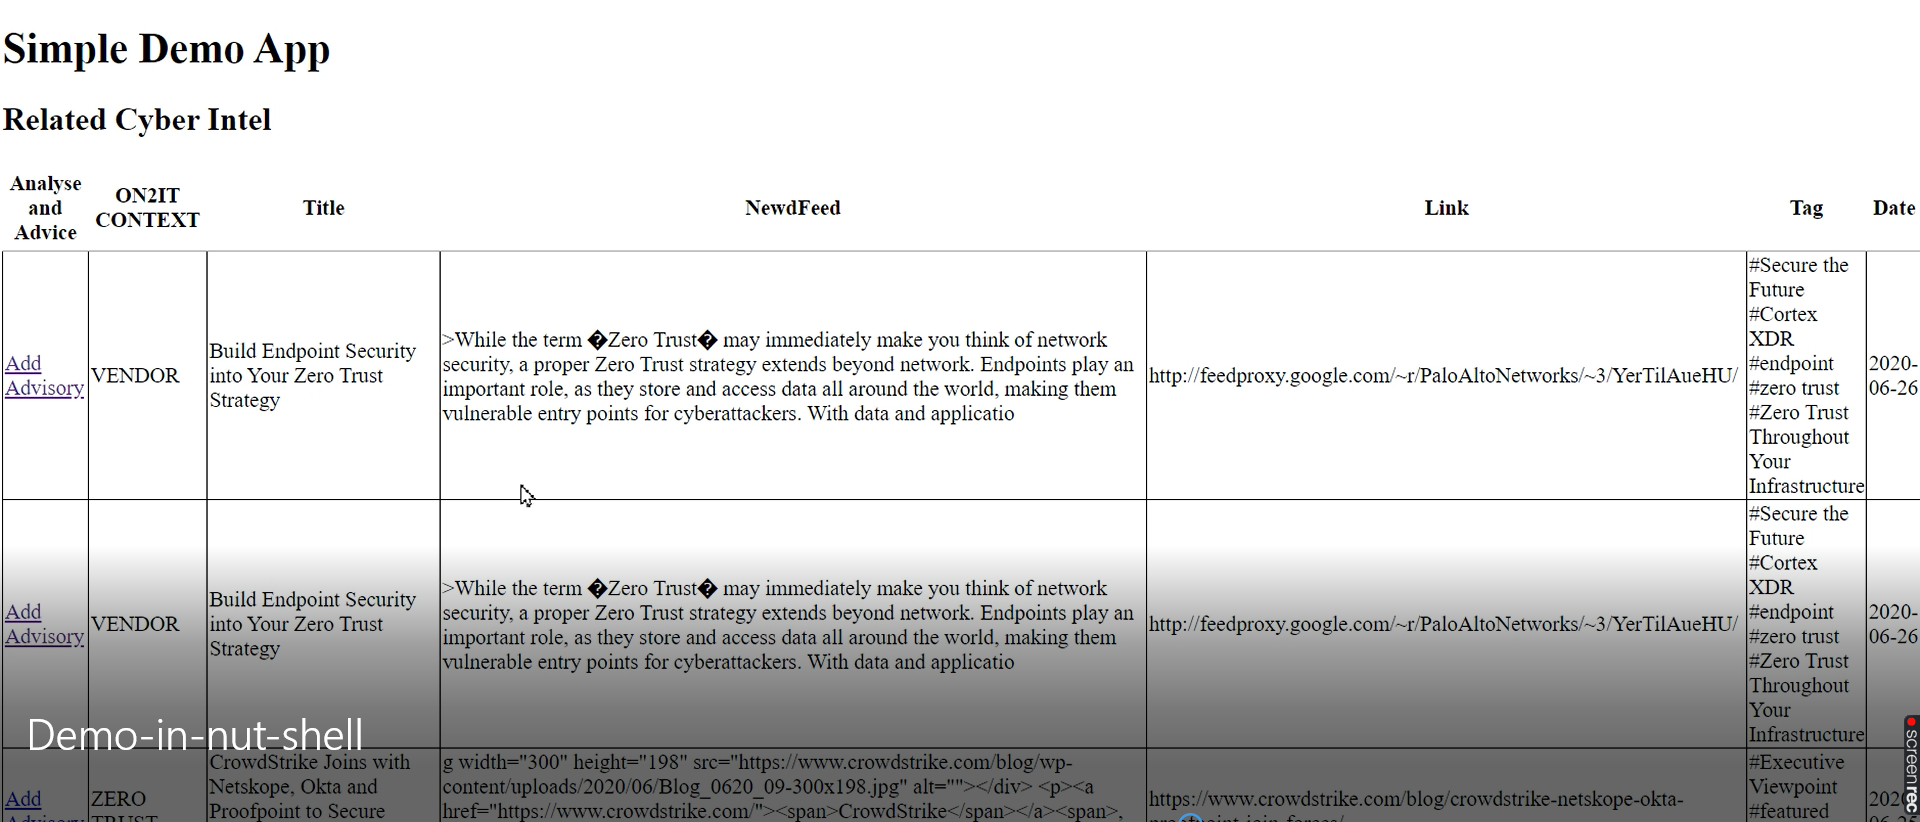
\includegraphics[width=1\linewidth]{Figures/tag-intel.PNG}}
    \caption{Screenshot of the artefact: List of co-related news}
    \label{fig:tag-intel}
\end{figure}
 \FloatBarrier
 
 

An analyst can co-relate similar cyber newsfeed items, 
he can perform impact analysis and root cause analysis for the cyber newsfeed item, which is manual. 
Finally he can add all his work and can add available solution to the cyber newsfeed items as a draft advisory as depicted in FIGURE \ref{fig:add-advisory}.

\begin{figure}[ht]
    \centering
    \fbox{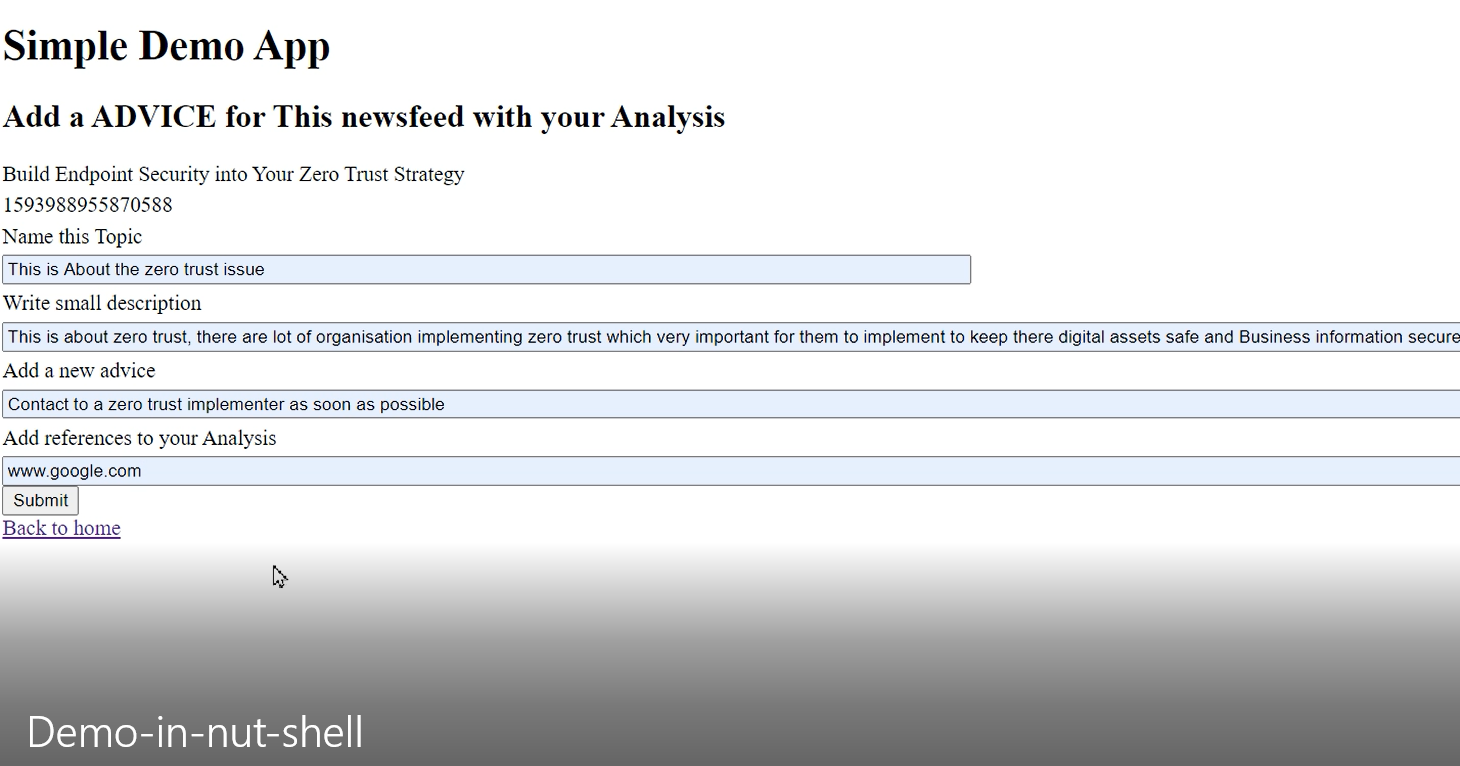
\includegraphics[width=1\linewidth]{Figures/add-advisory.PNG}}
    \caption{Screenshot of the artefact: Demo GUI to add Advisory}
    \label{fig:add-advisory}
\end{figure}
 \FloatBarrier


After analysis and adding advisory of an organisation-specific cyber newsfeeds, 
the cyber analysts can refer to the list of cyber newsfeeds Intels along with advisory being created as 
as shown in FIGURE \ref{fig:analyst-advisory-demo} and store them in the  GitHub repository for editorial validations. After editorial validations, the organisational-specific contextula cyber intels can be delivered to the stakeholders.

 
\begin{figure}[ht]
    \centering
    \fbox{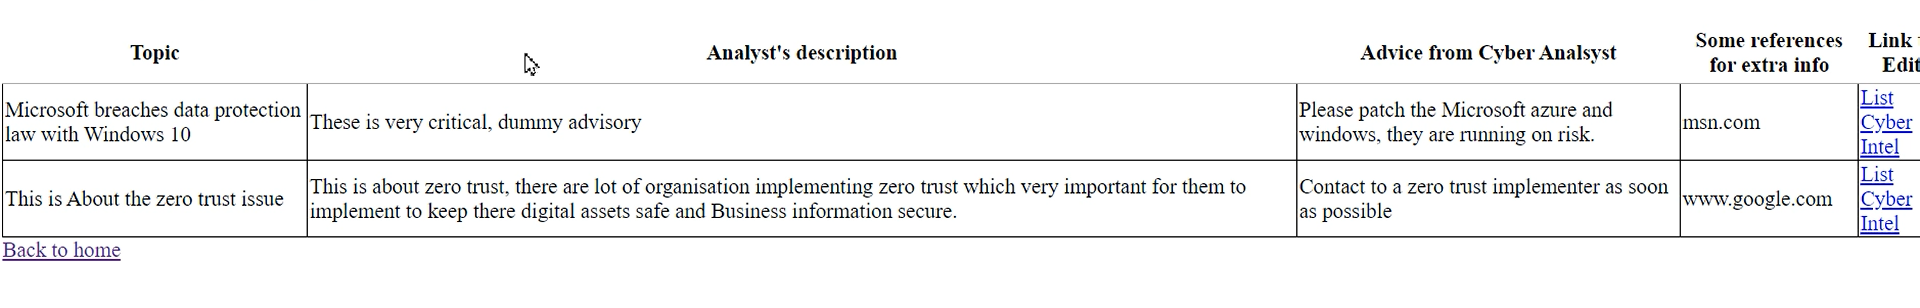
\includegraphics[width=1\linewidth]{Figures/analyst-advisory-demo.PNG}}
    \caption{Screenshot of the artefact: Demo GUI to List cyber newsfeed Intel}
    \label{fig:analyst-advisory-demo}
\end{figure}
 \FloatBarrier

Analyser \& Advisory Module helped to make the cyber newsfeed brief \footnote{A group or list of cyber news items}, which is a deliverable Intel for the stakeholders. 
The stakeholders receives the organisation-specific  context which the cyber analyst configured during the activities described in the Processor module. 

\subsection{Prototype on accessing the data source quality}
\label{quality_source}
For assessment of data sources I proposed to use one of the quantitative metrics listed in chapter  
\ref{Chapter7_literature-review}
TABLE \ref{table:quantitative}.
One of the metrics called \enquote{Extensiveness} was selected to be   implemented for this artefact because this parameter was first in the sequence. The complete formula and description for \enquote{Extensiveness} is mentioned in TABLE  \ref{table:source-quality}. 

The formula \textbf{extensiveness parameter} $p_1$ evaluates the number of extra parameters which are filled in for a Really Simple Syndication (RSS)\footnote{\url{https://validator.w3.org/feed/docs/rss2.html} } feed. 
\textbf{Symbol} $o_i$
is the sum of the filled-in optional
properties in \textbf{a cyber newsfeed} i. The \textbf{ total number of
messages shared by the source} is $z$. 
Max $y_i$ 
is the \textbf{maximum number
of optional properties} defined for this specific type of message i by
 RSS feed.
%% This file contains only a table.
%% this file is included into Chapter8

\begin{table}[htbp!]
   \setlength{\arrayrulewidth}{0.1mm}
    \setlength{\tabcolsep}{5pt}
    \renewcommand{\arraystretch}{1.0}

    \centering{}
 
    \caption{Source Quality metrics: Qualitative}
    \label{table:source-quality}
    
    \begin{tabularx}{\linewidth}{| p{1.11cm}|p{2.50cm}|p{4cm}|p{1.05cm}|p{3.7cm}|} 
    
%    |a|>{\columncolor[HTML]{FFFFFF}}C|C|C|
     \arrayrulecolor[HTML]{06000A}
        %% Table Body
        \hline
        \rowcolor[HTML]{5789F3} 
        \multicolumn{5}{|c|}{Quantitative based metrics} \\
        \hline
        
        \rowcolor[HTML]{ECB4E8} serial \# & Parameter type & Parameter Description & Symbol & Math Formula  \\
        \hline
 1	&	Extensiveness	&	Evaluates how many optional parameters are filled in	&	p1	&	\[p1 = \frac{1}{z}\sum\limits_{n=1}^{z}(\frac{oi}{\max y_i}) \]	\\ 
  
\hline
    \end{tabularx}

\end{table}







\section{Conclusion}
This concludes the chapter \ref{Chapter8_artefact-design} and with this,  the model of processes and activities required in the artefact prototype of \enquote{Cybernewsfeed Technology} was ready.
The steps taken and augmentations considered while designing and simulating the artefact on AWS cloud with the help of MySQL, Apache and PHP was also mentioned.
After the creation of this artefact the next research step is the evaluation of the artefact which is presented in next chapter.







% Chapter 

\chapter{Artefact Evaluation} % Main chapter title

\label{Chapter9_artefact-evaluation} % For referencing the chapter elsewhere, use \ref{Chapter9} 

\section{Introduction }
This chapter is about the evaluation process of the work done in section \ref{New artefact prototype} in  chapter \ref{Chapter8_artefact-design}, \nameref{Chapter8_artefact-design}  to create the artefact \enquote{Cybernewsfeed Technology}. The relevance of the created artefact \enquote{Cybernewsfeed Technology} is validated by the Focus Group and the approach and outcome of the validation process is explained in this chapter.

\section{Evaluation Process}
As mentioned in chapter \ref{Chapter6_research-approach} \nameref{Chapter6_research-approach}, this research was designed to perform validation using Group Support System (GSS) under the Design Science Research (DSR) framework. 
For the validation of artefact, this thesis took focus group
\citep{langford2012qualitative} discussion approach for GSS. 
To run the GSS validation,
it was needed to have a focus group
\citep{langford2012qualitative} 
of six to eight people with similar background in the cybersecurity threat intelligence domain and who are willing to uncover a range of perspectives and experiences. 
The shortlisted  focus group participants as per list of Appendix \ref{AppendixChapter9}, \nameref{AppendixChapter9}
 were invited to participate in the group session. 
The pre-read materials, scope, agenda and presentation to be used during the session were shared upfront with the participants. 
The session was scheduled on 15th July 2020, 
Wednesday between 18:00 to 20:00 hours via an online Zoom meeting with the help of experienced moderators who captured the broad range of views of the group.


\subsection{Scope and Objective}
The scope of this Group support system research was to demonstrate and validate the prototype which had been build. 
This group session took approximately two hours, 
starting with prototype demo and  presentation.
 After that an open discussions about the design and functionality of the artefact among the focus group. 
In the end we ran an online survey to let the Focus group share the expertise, 
perspective and experience on the topic.

\subsubsection{Objectives of the session}
\begin{itemize}
    \item Primary objective is to examine the automated Cybernewsfeed tooling modules that collects,
ingests and parses relevant cyber information based on adjustable parameters.
    \item Secondary objective of the survey is to get insight on the form, frequency, pricing and content of such a cybernewsfeed Brief.
\end{itemize}

\subsubsection{Survey type}
I have made use of GSS because GSS is very craftful for making use of experts or focus group of people that are geographically spread but can attend physically. Choosing a Group system support(Focus group) mechanism ensured that participants represented all the three levels of stakeholders to discuss on the topic of \enquote{Cybernewsfeed Technology}. During the Focus Group discussion, we captured the responses of Focus Group participants using Meeting Wizard\footnote{\url{https://www.meetingwizard.nl/}} tool and the professor Yuri Bobbert who is specialised in GSS was the moderator of this session. The GSS session was observed by Willy Lund\footnote{An ON2IT facilitator} so that the execution of GSS session goes according to the academic principles. 

\subsubsection{Agenda}
The Agenda set for two hours for the GSS was structured as below.

\begin{itemize}
    \item The artefact prototype Expectation Setting - 5 Min
    \item Understanding The Prototype - 15 Min
    \item Open Discussion by Focus group about the prototype - 15 Min
    \item Demo: Cybernewsfeed Technology(The Artefact) - 15 Min
    \item Survey: To collect Focus group opinion - 70 Min
\end{itemize}

\subsubsection{Demo Link}\label{Demo Link}
In the link below, you can find the demo video of the tool which is a pre-recording of the tool \enquote{Cybernewsfeed Technology}. This demo video was presented to the Focus group.
\begin{itemize}
    \item \url{https://drive.google.com/file/d/1P8eFg7wJtW55Z3QfAO8qCHbZJqlao9Q6/view?usp=sharing}
\end{itemize}



\subsubsection{Survey Questions in GSS}
\begin{enumerate}
    \item What is the industry that you are working in? (Brainstorm)
    \item At what level are you positioned in your organisation? (Flipboard)
    \item At what level are you positioned in your organisation? (Voting)
    \item How would you rate the quality? (Flipboard)
    \item How would you rate the quality of the end product? (Voting)
    \item Requirement setting. (functional and technical) (Brainstorm)
    \item What is your experience with such a technology? (Flipboard)
    \item What is your experience with a Cybernewsfeed technology? (Voting)
    \item How interested are you in such a cyber newsfeed? (Flipboard)
    \item Please rate your interest in such a cyber newsfeed. (Voting)
    \item Ordering of the cyber newsfeed content items' relevance. (Flipboard)
    \item Relevance of the cyber newsfeed content (what is your preference?) (Voting)
    \item Frequency of the Cybernews feed. (Flipboard)
    \item Selecting the frequency of the cyber newsfeed. (Voting)
    \item Media form of the cyber newsfeed. (how to receive) (Flipboard)
    \item Selecting the media form. (Voting)
    \item Pricing range of the cyber newsfeed technology. (Flipboard)
    \item Pricing of the Cybernewsfeed technology + advisory. (Voting)

\end{enumerate}

\section{Artefact Evaluation Results}\label{Artefact Evaluation Results}
In this section we have mentioned the collected feedbacks about the artefact \enquote{Cybernewsfeed Technology}. These feedbacks higlights about the following two things: 1) participant's familiarity with the similar product and 2) demand and desire of the cybernews brief created via such a cybernews feed technology. The parameters for GSS evaluation are mentioned in the survey questions.  We have also captured additional functional and technical requirements for the next iteration of the artefact development.

\subsection{Representation and Background of Participants of the Focus group}
This section reflects the answer to the survey question number one, two and three. It showed that the Focus group represents four different industries:
\begin{enumerate}
    \item Healthcare
    \item Finance
    \item Government
    \item Chemical
\end{enumerate}
 About the background of the participants, the participants in the group were functional as stakeholders at multiple levels:
 \begin{itemize}
     \item Tactical/Management: 3
     \item Strategic/Board: 6
     \item Operational: 2
 \end{itemize}
\subsection{Additional functional and technical requirements}
This section lists the answers to the survey question number six, where participants expects additional functionalities on the top of existing functionalists in the demo artefact. Participants shared these following  functional and technical requirements.
\begin{enumerate}
    \item Additional technical requirements you would like to see/have?
    \begin{enumerate}
        \item Decision tree info on the level of filtering.
\item Ranking of cyber newsfeed items. 
\item  Risk Rating of Vulnerabilities.
\item  Expected complexity to implement.
\item  Maintenance of the decision tree.
\item Continuous monitoring and reporting of new vulnerabilities.
\item  Relevance (higher/lower) in terms of relevance to the existing landscape, processes, policies, risk appetite etc.
\item  Technical value score of software supplier (past).
\item  The current and trending hot topics in cyber world. 
\item  Information about the RTO\footnote{RTO \url{https://en.wikipedia.org/wiki/Disaster_recovery\#Recovery_Time_Objective}}, RPO\footnote{RPO \url{https://en.wikipedia.org/wiki/Disaster_recovery\#Recovery_Point_Objective}} and Availability in case of known security incidents.

\item Reliable and secure information sources.
\item Add  information relating to OWASP\footnote{Open Web Application Security Project (OWASP)\url{https://en.wikipedia.org/wiki/OWASP} }, SANS25\footnote{SANS\footnote{\url{https://en.wikipedia.org/wiki/SANS_Institute}} top Top 25 Software Errors\url{https://www.sans.org/top25-software-errors}}, General Data Protection Regulation (GDPR)\footnote{\url{https://en.wikipedia.org/wiki/General_Data_Protection_Regulation}} , ISO27001 and various other legal requirements.
    \begin{itemize}
        \item Reference, if the vulnerability relates to elements in these domains. Related to if an organisation has to adhere to any of these
        principles.
     \item How will patch updates if any be performed?
    \end{itemize}

\end{enumerate}
    \item Additional functional requirements you would like to see/have?
    \begin{enumerate}
        \item Dashboard on supplier, vulnerability history and speed of solving.
        \item Role based management (managing info supply).
        \item Ability to customize / filter feeds based on "need to know" and "nice to know / trend" information.
        \item Ability to list and rank data sources.
    \end{enumerate}
\end{enumerate}


\subsection{Prototype Demo feedback}
 The artefact demo video of 15 minutes was played to show the end-to-end functionalities of the Collector, of the Processor and of the Analyser \& Advisory modules. 
The general feedback of the Focus group participants were positive and the concept of making such a prototype was rated as new. 
Some comments captured from Focus group participants is shown in FIGURE \ref{fig:feedback}.

\begin{figure}[ht]
    \centering
    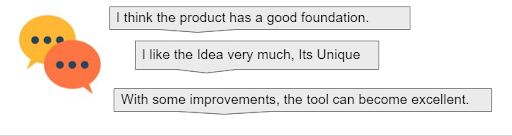
\includegraphics[width=.65\linewidth]{Figures/feedback.png}
    \caption{Focus group Comments on the artefact demo}
    \label{fig:feedback}
\end{figure}
 \FloatBarrier

\subsection{Familiarity with such product}
\label{ref:familiar}
This was the reflection of the survey question number seven and eight. All the participants in the Focus group were familiar with similar technology and some of them have already used. 
There was no one who is not aware of cyber intel technology. 
Participants familiarity with such technology ensured that the validation process in on right track and everyone understands, and can respond to the questions related to the demo product. In FIGURE \ref{fig:product-familarity}, the pie chart representation of the individual responses from the participants is shown.

\begin{figure}[ht]
    \centering
    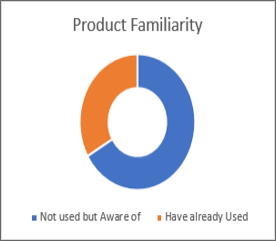
\includegraphics[scale=0.6]{Figures/product-familarity.png}
    \caption{Familiarity: Group Knowledge on similar technology }
    \label{fig:product-familarity}
\end{figure}
 \FloatBarrier

\subsection{Interest in such product}
\label{sec:interest}
This was the reflection of the survey question number nine and ten. Here I have checked the interests of the group for such a product and the results were very interesting. 
Half of the group was slightly interested 
and the other half were very interest. 
There was no one from the group who was not interested in such a product. 

\begin{figure}[ht]
    \centering
    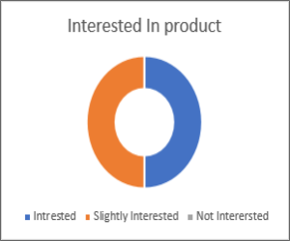
\includegraphics[scale=0.6]{Figures/product-interest.png}
    \caption{Interest: in similar technology}
    \label{fig:product-interest}
\end{figure}
 \FloatBarrier

\subsection{About the product concept}
\label{sec:concept}
 The topic of survey questions four and five was the validation of the product concept. 
 The questions where answered by selection one of the following options: Excellent, Good, Average or Poor. 
 In addition to the voting option there was a text field available for additional feedback. 
 Of the six participants three (50\%) voted `Good` and three (50\%) voted `Average` 
 (See FIGURE \ref{fig:product-concept}).
The free text feedback of the six participants
is included below.

%This was the reflection of the survey question number 4 and 5. For validating the product concept, we used voting options and captured the additional information as text.
%According to the responses captured from the participants based on the rating of Good, Average, Excellent or Poor, here is the list. The group's comments has been presented in its format before the reader.

\begin{figure}[ht]
    \centering
    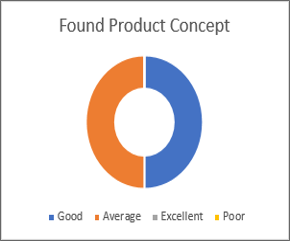
\includegraphics[scale=0.6]{Figures/product-concept.png}
    \caption{Concept: About the artefact demo during GSS}
    \label{fig:product-concept}
\end{figure}
 \FloatBarrier

 \begin{enumerate}
 \item Good
 \begin{enumerate}
\item Missing rating of the reported data. Also what is the quality of this reported data. This information will improve
this tool further.
\item Based on the limited amount of information so far I thing the product has a good foundation. I see however some
improvements in the contextualization of the information on operational level (maybe mapping against a CMDB). I
also suggest a feedback loop (measures the effectiveness and quality of the risk mitigation/information put in
context) and the risk assessment (probability, risk level, Vulnerability, Impact, Frequency) and prioritization of risk
mitigating actions proposed by the tool.
\item Filling in the raw data based on the short data seems like it could become a strenuous task, especially with
multiple sources. 
\\- Add a list of possible sources based on their quality rating and information. 
\\- Including and
elements related to the Look and feel and intuitive design are important
  \end{enumerate}
   \item Average 
   \begin{enumerate}
      
  
    \item Decision tree role based advice (agile) just in time (if i'm developing other feed is needed than in Production)
 \item The decision tree is key for the value of the tool. that will make the tool good. With improvements on the
reporting part, considering risks, prioritisation and stakeholder management, the tool can become excellent.
 \item Can consist of some additional requirements for follow up of actions, prioritization, branch specific information,
continuous run that presents me actionable information as soon as it becomes available. The UX should be way better. Do not invite me to use with this GUI.
 \end{enumerate}
   \item Excellent 
   \begin{enumerate}
       \item Not Applicable 
   \end{enumerate}
   \item Poor
   \begin{enumerate}
       \item Not Applicable 
   \end{enumerate}
 \end{enumerate}



\subsection{Desired cyber newsfeed type}
\label{sec:desire}
This was the reflection of the survey question number 11 and 12. In this section, we captured the newstype by priority for the type of news listed in TABLE \ref{tab:stakeholder-news}. 
The group's interested and their comments in as it is format has been presented before the reader. In FIGURE \ref{fig:product-desire}, the desired cyber newsfeed type is listed by priority.

\begin{figure}[ht]
    \centering
    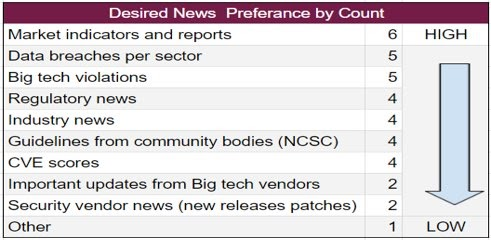
\includegraphics[width=.75\linewidth]{Figures/product-desire.jpg}
    \caption{Desired cyber newsfeed type: Priority high to low}
    \label{fig:product-desire}
\end{figure}
 \FloatBarrier
\begin{enumerate}
    
    
     \item Market indicators and reports
     \begin{itemize}
  \item This is nice to now what the market trends are.
     \end{itemize}
 \item Data breaches per sector
 \begin{itemize}
  \item Especially developments in the hacker "industry" is quite relevant.
\item Due to my interest in data privacy, I'm ineterested in data security breaches and the reasons why the occur.
\item In my work as consultant i work on a project for a specific sector longer then a year. It is interesting to know the
data breaches for this specific sector.
     \end{itemize}

 \item Big tech violations
 \begin{itemize}
     \item Gain relevant in the context of data privacy.
 \end{itemize}

 \item Regulatory news
  \begin{itemize}
\item Important to manage the organisation.
\item Especially regarding the intersection between data privacy and data security. The GDPR e.g. requires sufficient
technical and org. measures around security (just one example).
\item It depends, it can be interesting to have this news but not always. Nice to have.
 \end{itemize}
 \item Industry news.
  \begin{itemize}
 \item As a consultant working on a project for a specific sector longer then a year. It is interesting resting to have the
news for this specific industry.
 \end{itemize}
 \item Guidelines from community bodies (NCSC).
 \begin{itemize}
 \item Good independent info.
 \end{itemize}
 \item CVE scores
 \begin{itemize}
\item General check before going live.
\item You want to know what the new vulnerabilities and exposures are and what there score and impact and what to
do about it?
\end{itemize}
 \item Important updates from Big tech vendors.
 \begin{itemize}
\item Nice to new what the updates are from the big tech vendors and what new solutions they have to implement at
your customers.
\end{itemize}
 \item Security vendor news (new releases patches).
 \begin{itemize}
\item Vendor news are for operational security  officers.
\end{itemize}
 \item Other.
 \begin{itemize}
\item Company specific items based upon business function, tool, supplier and competitor.
\end{itemize}
\end{enumerate}


\subsection{Desired media}
\label{sec:media}
This was the reflection of the survey question number 15 and 16.
As shown in the FIGURE \ref{fig:product-media}, the first preferred delivery media channel according to the Focus group is 
\textit{Messaging (Signal, WeChat)}. 
Second preference is \textit{e-Mail} media and the
third preference is via \textit{Security Operations Center (SOC) portal}. 
\begin{figure}[ht]
    \centering
    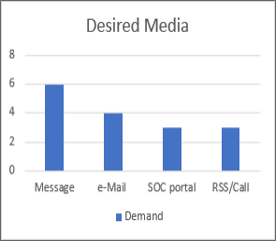
\includegraphics[scale=0.6]{Figures/product-media.png}
    \caption{Desired Media: Across available options}
    \label{fig:product-media}
\end{figure}
 \FloatBarrier
\textit{Messaging (Signal, WeChat)} 
is most preferred because the urgent issues having high risk can be communicated direct for immediate action.
\textit{e-Mail} is considered to be good for weekly communications on important cyber news items. 
With the \textit{SOC portal}, 
the items can be directly pushed to SOC dashboard. 
Other media like \textit{direct call} got importance in case of very urgent issues.
\textit{RSS} feed was the least desired media. 




\subsection{Desired Frequency}
\label{sec:frequency}
This was the reflection of the survey question number 13 and 14. We collected the desire about the frequency of cyber news items getting published to stakeholders 
according to FIGURE shown \ref{fig:stakeholder-problem-domain} in chapter \ref{Chapter4_problem-domain}, \nameref{Chapter4_problem-domain}. 

\begin{figure}[ht]
    \centering
    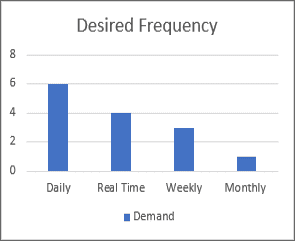
\includegraphics[scale=0.6]{Figures/product-frequency.png}
    \caption{Desired Frequency: Of the cyber newsfeed}
    \label{fig:product-frequency}
\end{figure}
 \FloatBarrier
Here is some interesting information provided by the Focus group.

\begin{itemize}
    \item Daily
        \begin{itemize}
            \item for direct important patches (e.g. Microsoft today)
            \item Daily feeds for information on cyber risks that require quick action
        \end{itemize}
    \item Others
        \begin{itemize}
            \item Actually as soon as it is available.
            \item real time, otherwise daily, depends a bit on the type of information
            \item Instant messages (e.g. using SMS etc) for High risk events
        \end{itemize}
    \item Weekly
        \begin{itemize}
            \item stay up to date info
            \item A weekly summary of the most relevant news (prioritized)
        \end{itemize}
    \item Monthly
        \begin{itemize}
            \item dashboard
            \item kpi's
            \item metrics
        \end{itemize}
\end{itemize}



\subsection{Willingness to Spend}
\label{sec:pay}
This was the reflection of the survey question number 17 and 18. The last input requested from the Focus group was about the willing to spend.  
The insight to this topic is very interesting as it can help the artefact to be productive and commercial.
\begin{figure}[ht]
    \centering
    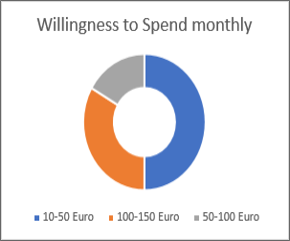
\includegraphics[scale=0.6]{Figures/product-cost.png}
    \caption{Cost of Cyber Intel produced by the  artefact}
    \label{fig:product-cost}
\end{figure}
 \FloatBarrier

\begin{itemize}
    \item 10-50 Euro
        \begin{itemize}
            \item is very much depending on how many users, 
            information wideness, 
            focused on the job element,
            measurements, 
            decision tree in it, etc.
            \item Very much depends on the size of the organisation and the environment. 
            As long as it is scalable, 
            or maybe as part of a larger services 
            (Network Operation Center (NOC) or SOC service).
        \end{itemize}
    \item 100-150 Euro
        \begin{itemize}
            \item 1200-1800 per year is a no brainer for companies and gives clearance in the overload in data
            \item Price will be determined by (demonstrated) value of information, but my guess would be that this is a good
introduction price. The higher the quality and relevance of information, the more this service give value to clients and
a higher price. It is all about the Return on Investment (ROI) that will be determined by the license model and value
        \end{itemize}
    \item 50-100 Euro
        \begin{itemize}
            \item This is dependant on the features, look and feel intuitiveness, and the possibilities I have to make the information
applicable and/or use it to make decisions.
        \end{itemize}
    
\end{itemize}



\section{Conclusion}
The GSS session turns out to be very productive and there were new insights discovered about the product on various parameters.  This concluded about the approach taken in this thesis to validate the artefact. Here we also shared the outcome of the discussions held during the GSS which we captured via an online survey tool.


% Chapter 

\chapter{Findings, Conclusion, Limitations and Recommendation} % Main chapter title

\label{Chapter10_conclusion-recommendation} % For referencing the chapter elsewhere, use \ref{Chapter10} 

\section{Introduction }
 The goal of this chapter is to  provide the findings, conclusion, limitations  and recommendations for future research. 
 In \nameref{Research findings} (section \ref{Research findings}), 
 I provide the findings of the research relevant to the research question. 
 In \nameref{Research Conclusions} (section \ref{Research Conclusions}), 
 I have listed the conclusions from the viewpoint of rigor and relevance.
 In \nameref{Research Limitations} (section \ref{Research Limitations}), 
 I have listed the limitations of my research.  
 In \nameref{Future Recommendations} (section \ref{Future Recommendations}),
 the possibilities of exploration in this technology has been highlighted.
 
 
 \section{Research findings}\label{Research findings}
 There was one research question in chapter  \ref{Chapter4_problem-domain}, \nameref{Chapter4_problem-domain} section \ref{Research Question} and four sub-research questions in section \ref{Sub-research question}. Answers to these research questions listed in below section.
 
 \subsection{Research Question 1}
 \textbf{What  are  elements  for  a  cyber news feed  assessment  method  and  what  are  the parameters for automation?}
 \subsubsection{Answer}
The most important element for a cyber newsfeed assessment is the collection of cyber newsfeed items, followed by other methods as mentioned below and configuration of stakeholders specific tags in the tool is key to the automation. 

 \subsubsection{Sub-Research Question 1a}
\textbf{What are the core core concepts of cyber newsfeed and how do they work according to literature?}

\bigbreak

\textbf{Answer: } The core concepts around the cyber newsfeed are about the sources of the newsfeed, 
then the processes like collection, processing, analysis of the newsfeeds. 
In chapter \ref{Chapter7_literature-review},  \nameref{Chapter7_literature-review}
(section \ref{Existing practices, systems, and people involved in automated cyber newsfeed}), 
the essentials concepts according to the literature review has been provided in detail.
Chapter \nameref{Chapter7_literature-review}  also illuminate the related concepts of people and practices
(subsection \ref{Existing-practices}) in link with these processes. 

 
\subsubsection{Sub-Research Question 1b}
\textbf{How does the vendor field of automated cybernewsfeed suppliers of artefacts look like according to the literature?}

\bigbreak

\textbf{Answer: } This study looked at 17 different threat intelligence tools in chapter \ref{Chapter7_literature-review}, \nameref{Chapter7_literature-review} (TABLE \ref{tab:tip-list}) provided by the different vendors. Among the tools, the collection of data is the only common behaviour. Other downstream activities like processing and analysis require customisation and configuration organisation-specific newsfeeds. The answer to this question is  in chapter \ref{Chapter7_literature-review}, \nameref{Chapter7_literature-review} (subsection \ref{Existing systems}).
 



 \subsection{Research Question 2}
 \textbf{How to make a prototype to filter contextual cyber Intelligence,
 perform automatic relevance tagging and 
 perform analysis for risk determination and advisory?}
 
\begin{figure}[ht]
\centering
    \fbox{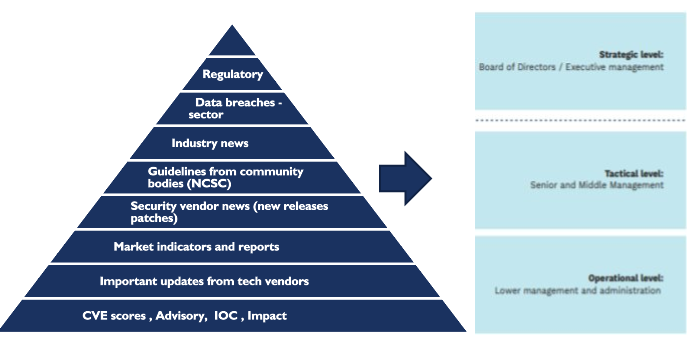
\includegraphics[width=.85\linewidth]{Figures/tailored.PNG}}
    \caption{Organisation-specific cyber newsfeeds to stakeholders}
    \label{fig:tailored}
\end{figure}
 \subsubsection{Answer}
There are three modules designed to achieve this, 1) the Collector, 2) the Processor and 3) the Analyser\&Advisory. 
A cyber analyst can pre-configure the required parameters of sources, contexts and tags with the help of a GUI. 
For writing advisory and editorial checks, the work flow has been proposed and a diagram has been provided for reference. 
The details are mentioned in chapter \ref{Chapter8_artefact-design},
\nameref{Chapter8_artefact-design}
(section \ref{Artefact and Artefact breakdown}). 
These three modules are: 
 

\begin{enumerate}
    \item \textbf{Collection Module:} 
    After evaluating 17 tools, 
    FreshRSS tool was used for collecting the newsfeed from various sources. 
    FreshRSS is an open source collection tool for RSS feeds and 
    can ingest cyber newsfeeds from multiple sources. 
    It has a GUI, has a database, is easy to deploy and is easy to customise.  

    \begin{figure}[ht]
    \centering
        \fbox{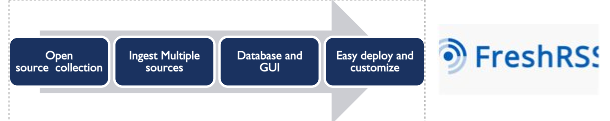
\includegraphics[width=.75\linewidth]{Figures/freshrss.png}}
        \caption{FreshRSS for Cyber newsfeed collection }
        \label{fig:freshrss}
    \end{figure}

    \item  \textbf{Processor Module: }
    For configuring the context specific to an area of particular interests of a stakeholder. 
    In this research we have filtered the first level of information 
    based on the contextualisation of Vendor and Non-Vendor specific information's.
    After filtration, 
    the relevant tagging was done by the tool with the vendor name, 
    for example TAG = Cisco, Microsoft or Amazon. 
    Tagged values of a particular interests of a stakeholder has been shown as a JavaScript Object Notation (JSON)  output with an example. 
    A JSON\footnote{JSON is a file format defined at \url{https://en.wikipedia.org/wiki/JSON}} 
    output of this processor module can be found
    in table format in Appendix \ref{json}. 
    The source code for archiving old data(cyber newsfeeds) collected  by the collector module is attached in Appendix \ref{AppendixChapter8} (section \ref{tag-archiving}).
    In Appendix \ref{AppendixChapter8} (section \ref{filter-context}), the SQL source code for filtering contextual data can be found. 
    For tagging of the more specific tags to a specific cyber newsfeed item, the PL-SQL function can be found in Appendix \ref{AppendixChapter8} (section \ref{tag-addtag}).
    To publish the processed cyber newsfeed via RSS feed to a cyber analysts, the source code can be found at \ref{AppendixChapter8} (section \ref{rss-send}).
    
    \item  \textbf{Analysis \& Advisory Module:}
    This module is designed to work with the output from the processor module and is human intensive. 
    First it will make correlations between similar cyber newsfeed items 
    either manually or automatic with the help of machine learning algorithms. 
    Then the cyber analysts, 
    using their skills and knowledge will perform additional research and provide additional information about the related risk and an advisory to act. 
     Finally the gathered cyber newsfeed contents will be validated together with editorial experts before dispatching the cyber intel to the stakeholders.

 \end{enumerate}


 \subsection{Research Question 3}
 
 \textbf{How to make a prototype for assessing the quality of the data sources?}
 \subsubsection{Answer}
 As mentioned in chapter 
 \ref{Chapter7_literature-review}, \nameref{Chapter7_literature-review}, 
 there are six qualitative 
 (TABLE \ref{table:qualitative}) 
 and ten quantitative 
 (TABLE \ref{table:quantitative}) 
 ways to evaluate the quality of cyber newsfeed sources. 
 The quantitative metrics will gain prominence over qualitative methods.
This has been explained in chapter \ref{Chapter7_literature-review} (section \ref{Existing methods available for data source quality assessment}).
 
In this research we have finalised one quantitative method \enquote{\textit{Extensiveness: Evaluates   how   many optional parameters are filled in}} as mentioned in   
TABLE \ref{table:source-quality} 
of 
chapter
\ref{Chapter8_artefact-design}, 
\nameref{Chapter8_artefact-design}.
In addition to 
\enquote{\textbf{Extensiveness}} 
as quantitative method, 
the Focus group suggested to capture the stakeholder's direct feedback as an evaluation parameter for cyber newsfeed source quality.

 \subsection{Research Question 4}
 \textbf{How to get the prototype validated for \emph{both 1) the design and 2) the output of this artefact} by the end users of specific organizations?}
 \subsubsection{Answer}
The prototype was validated by the Focus group using GSS, The chapter \ref{Chapter9_artefact-evaluation}, \nameref{Chapter9_artefact-evaluation},
lists the results of the  validation. 

\section{Research Conclusions} \label{Research Conclusions}
In this section, I presented my research conclusions.
My main conclusions are based 
upon the analysis of 
the collected research data. 
I categorized my conclusions as follows: 
1) first part on the relevance for the stakeholders and 
2) second part on the rigor applicable to this artefact 
\enquote{Cybernewsfeed technology}. 

\subsection{Conclusions on the relevance of the \enquote{Cybernewsfeed technology}}

%As mentioned in chapter \nameref{Chapter6_research-approach} my research needs to be relevant.
Below are the conclusions on the relevance of the 
\enquote{Cybernewsfeed technology} provided by the stakeholders 
in the Group Support System (GSS) sessions.

Outcome of the GSS was that the stakeholders indicated 
that getting organisation-specific information via the cyber newsfeeds
is important to them (section \ref{sec:interest}). 
The proposed tool  
\enquote{Cybernewsfeed technology} was regarded as fullfilling
this need (\ref{sec:concept}).

Outcome of the GSS was that the stakeholders currently do not use
similar technology to fulfill their need (section \ref{ref:familiar}).
The stakeholders stated that they would purchase similar technology
if it was available to them (section \ref{sec:pay}).

For the technology itself to be relevant to the stakeholders, 
it needs to provide information on a daily basis
with exception of the critical information.
Notification of critical information needs to be real-time 
to be relevant to the stakeholders (section \ref{sec:frequency}).
Real-time notification is preferred 
by the stakeholders via instant messaging (section \ref{sec:media}). 

%The topic of data privacy and data security has the main interest with the stakeholders (section \ref{sec:desire}).


 %\subsubsection{Relevance Conclusion 1} 
 %The results indicate that getting organisational-specific cyber newsfeeds is eminent   for the stakeholders and there is a need of similar technology like this tool \enquote{Cybernewsfeed technology}.  
    

%\subsubsection{Relevance Conclusion 1} According to the target group exercise that we did, actionable cyber intel is important for the stakeholders because of the .....

%\subsubsection{Relevance Conclusion 2} 
%Based on the feedback on interests from the stakeholders. 
%From an organizational point of view, 
%they are knowing but they don't use it yet, 
%so there is a need.

%\subsubsection{Relevance Conclusion 3}
%The stakeholders are willing to pay  money 
%but they are not yet using a similar service.

%\subsubsection{Relevance Conclusion 4} 
%The stakeholders that I have interviewed during the GSS are looking forward to more strategic and tactical news, rather than the operation news. This could be a case because they functional at strategic and tactical level and they have more need for strategic and tactical level of information.

%\subsubsection{Relevance Conclusion 5} 
%Most desirable frequencies to receive such a cyber neewsfeed is daily. 
%The stakeholders want to receive the information in real time for the %critical cyber newsfeed.

%\subsubsection{Relevance Conclusion 6}
%According to the target group exercise, the most desired media is messaging. 

%\subsubsection{Relevance Conclusion 7} 
%Data privacy is perceived as the most 
%important concerns for the stakeholders.

\subsection{Conclusions on the rigor of the \enquote{Cybernewsfeed technology}}




%\subsubsection{Rigor Conclusion}



In my literature research I found a limited amount of
academic sources on the topic of cyber intelligence 
within the scope of my research.
My research is a contribution to the existing body of knowledge.
The insight that the solutions similar to \enquote{Cybernewsfeed technology: REVEAL}
requires organisation-specific configuration and that the solution
needs editorial functionalities to tailor the content,
are an addition 
to the existing body of knowledge.

%There are very few academic research done in cyber intel because I did not find many literatures. 
%I made a contribution in adding a new knowledge source by concluding that such cyber intel sharing technologies like \enquote{Cybernewsfeed technology: REVEAL} requires  organisation-specific configurations functionalities and in built editorial functionalites to tailor the content of newsfeeds. 
%Optimum output from the \enquote{Cybernewsfeed technology} can be achieved with the help of configurable parameters and custom defined algorithms.



According to my literature research and stakeholders feedback only tools capabilities are not sufficient to deliver organisation-specific newsfeeds, a role of the cyber analyst and editor are also very critical.
%for the analysis and providing any applicable solution for the specific cyber news feed intel.

%It can be concluded that there are some important factors to consider when designing and developing the 
%\enquote{Cybernewsfeed technology} 
%for optimum output. 

%\subsubsection{Rigor Conclusion 4}
%There are two configurable tasks required to run this tool. 1) Configuration of data sources and 2) configuration of tags required to filter the specific items. 



\section{Research Limitations}\label{Research Limitations}

%\subsection{Limitation 1}
Prototype on assessing the data source quality in chapter \ref{Chapter8_artefact-design} section \ref{quality_source} could not be implemented or validated. There was not enough data and time to assess the quality information of the cyber newsfeed sources. 

%\subsection{Limitation 2}
%The technology needs more functional and technical capabilities to be %operational and a productive product. 


%\subsection{Limitation 3}
%To calculate automated risk determination, 
%implementation of decision tree 
%is required and has not been covered in this paper.

%\subsection{Limitation 4}
%The Graphical User Interface (GUI)\footnote{GUI according to Wikipedia \url{https://en.wikipedia.org/wiki/Graphical_user_interface}} in this artefact may not be acceptable by the users, as it is only for demonstration and can be improved with better screens.

%\subsection{Limitation 2}
The Focus group has six participants for the representation of stakeholders population.
One could argue if six participants are enough,
where I think the level of expertise of the participants
is more important then the amount of participants.

%\subsection{Limitation 3}
The research has been executed in coordination with one organisation  instead of multiple organisations, I could have collected more requirements for the artefact.


%\subsection{Limitation 4}
The research was executed in six months and I feel I could have done better with more time and due to less time the results of this tool has not been used in a real life environment, 
the tool is still in incubation phase. 

%\subsection{Limitation 5}
I am a software developer and not a cybersecurity expert,
but when I started my research, slowly learned and gained the knowledge in the field of cybersecurity, 
 and this improved my research work.



\section{Recommendations for future research}
\label{Future Recommendations}


The curiosity to understand the missing influence of such tools among the stakeholders could be an interesting illumination.
To me this is an indication that there is a need that is not yet met. 
It is my recommendation to further study the root cause of this need
with the stakeholders.
I  would also recommend to improve the prototype 
and develop it in an iterative software development way into a more mature solution.

Another direction could be to improve the maturity of the solutions 
by combining both cyber security and software Engineering knowledge, for example to implement `automatic risk analysis and determination` or `automatic source sanitation`.
%In my opinion, by adding this knowledge can  
%done in the scientific way that I used in my research.
 

\section{Personal Reflection}


I have learned a couple of things about myself during my
Executive Master education at the Antwerp Management School. 
Knowledge wise I have gained a broader and holistic view on the IT related corporate practices; 
and have learned to apply academic and holistic approach to any problem. 
I learned to be resilient during the thesis, 
improved myself in adverse situations, 
for instance I lost my new job, had hopes in future so started to learn new technologies, and then the continuous learning has became a part of me.

I never considered myself as a good writer, 
never wrote more than two pages in English. 
I had problem understanding Dutch, but things have changed; I can write a fair amount of literature, can converse in Dutch language. 
I am also reflecting on my presentation to the CEO and learnt that I should prepare such meetings better and not getting distracted before the critical presentations.

\newpage
\centering \section*{Thankyou}
\centering \subsection*{With the feeling of being thankful}
 \begin{figure}[htbp!]
    \centering
        \fbox{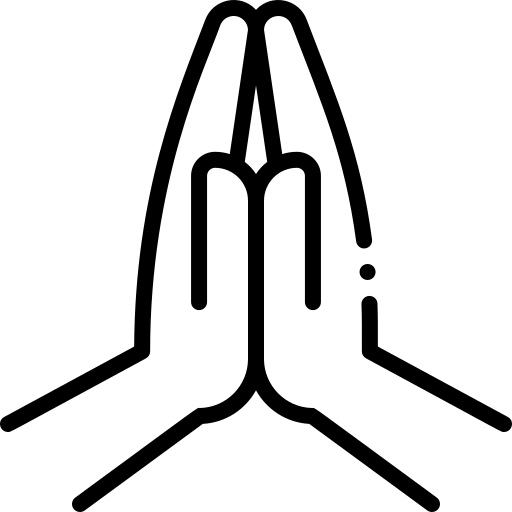
\includegraphics[width=.20\linewidth]{Figures/namaste.png}}
        \caption{}
        \label{fig:namaste}
    \end{figure}
\FloatBarrier





%\include{Chapters/test_table}
%\include{Chapters/ExampleChapter1}

%----------------------------------------------------------------------------------------
%	THESIS CONTENT - APPENDICES
%----------------------------------------------------------------------------------------

\appendix % Cue to tell LaTeX that the following "chapters" are Appendices

% Include the appendices of the thesis as separate files from the Appendices folder
% Uncomment the lines as you write the Appendices


\chapter{Executive Summary} % Main appendix title

\label{AppendixA} % For referencing this appendix elsewhere, use \ref{AppendixA}

\section{\enquote{Scattered \& Raw} cyber information}\label{fig:cyber-feed-info-appendix}


\begin{figure}[b!]
  \centering
\fbox{\includegraphics[width=1\textwidth]{Figures/cyber-feed-info.PNG}}
  
\end{figure}
\FloatBarrier

\section{\enquote{Actionable} cyber intelligence}\label{fig:cyber-feed-intel-appendix}


\begin{figure}[b!]
  \centering
\fbox{\includegraphics[width=1\textwidth]{Figures/cyber-feed-intel.PNG}}

  
\end{figure}
\FloatBarrier
\bigbreak

\section{Requirement}
%% This file contains only a table.
%% this file is included into Chapter8

\begin{table}[htbp!]
   \setlength{\arrayrulewidth}{0.1mm}
    \setlength{\tabcolsep}{5pt}
    \renewcommand{\arraystretch}{1.0}

    \centering{}
 
    \caption{Requirements: Cybernewsfeed Technology}
    \label{table:Cybernewsfeed-technology}
    
    \begin{tabularx}{1\linewidth}{| p{1.5cm}|>{\columncolor[HTML]{ECB4E8}}p{2.9cm}|p{3.0cm}|p{3.45cm}|p{1.5cm}|} 
    
%    |a|>{\columncolor[HTML]{FFFFFF}}C|C|C|
     \arrayrulecolor[HTML]{06000A}
        %% Table Body
       
        \hline
         \rowcolor[HTML]{BFCEED} Module & Requirements & What? & Why? & MoSCoW priority \\
        \hline
     \multirow{4}{*}{Collector}  & Language Support	&	Support various languages.	&	To not miss intel in other languages	&	Must have	\\\cline{2-5}
& Data Formats	&	Allow multiple data formats	&	To collect and process standard and recent formats	&	Should have	\\  \cline{2-5}
& Data Source types	&	Ingest from various sources	&	To cover broader sources of Intel	&	Must have	\\  \cline{2-5}
& Connection protocol	&	Support common protocols	&	To allow actual transfer To data	&	Must have	\\ \hline
\multirow{3}{*}{Processor} & Data structuring	&	Data mappings and Data format conversion	&	To ensure a common data format To enable further processing	&	Should have	\\  \cline{2-5}
&Contextualization	&	Possible to set context	&	To convert raw intel To specific intel	&	Must have	\\  \cline{2-5}
& Data Filtering	&	Be Able to Filter Data	&	Based on Adjustable Parameters	&	Must have	\\  \hline
\multirow{3}{*}{Analyser} & Co-relation	&	Group similar Intel	&	To reduce duplicity and improve granularity	&	Should have	\\  \cline{2-5}
& Analysis	&	Provide insights on tactics, severity and impact	&	To make the cyber intel actionable	&	Must have	\\  \hline
\multirow{3}{*}{Advisory} & Writing custom intel	&	Allow to write a new content for cyber newsfeed	&	To ensure that analyst can use his knowledge for providing details on cyber news	&	Must have	\\   \cline{2-5}
& Template Designing	&	Make design template for writing cyber intel and advisories	&	To allow flexibility in presentation of cyber Intel To further streams	&	Should have	\\   \cline{2-5}
& Feedback Collection	&	Collect internal and external user feedback	&	To check the quality and if the news is actionable	&	Could have	\\  \cline{2-5}
& Outbound Communication	&	Deliver Cyber newsfeed to users	&	To ensure cyber intel with advisory reach To destination	&	Must have	\\
        \hline
    \end{tabularx}

\end{table}







\label{tab:requirement-appendix}

% Appendix Template

\chapter{JSON newsfeed format to Table} % Main appendix title
\section{ON2IT Vendor Context}
\label{json} % Change X to a consecutive letter; for referencing this appendix elsewhere, use \ref{json}
\label{AppendixB} % For referencing this appendix elsewhere, use \ref{AppendixA}

\begin{table}[htbp!]
   \setlength{\arrayrulewidth}{0.1mm}
    \setlength{\tabcolsep}{5pt}
    \renewcommand{\arraystretch}{1.0}
\label{tab:json}
  %  \centering
   \resizebox{1.1\textwidth}{!}{ \begin{tabular}{|p{1.3cm}|p{1.5cm}|p{9.7cm}|p{4cm}|p{1.7cm}| p{4.3cm}|}
    \hline
        TAGS &  on2itcontext & newsfeed & title & pub\_date & link \\ \hline
        \#microsoft & VENDOR & Newly-elected politicians in Munich "have decided its administration needs to use open-source software, instead of proprietary products like Microsoft Office," reports ZDNet:

Munich began the move away from proprietary software at the end of 2006... By 2013, 80\% of desktops in the city's administration were meant to be running LiMux software. In reality, the council continued to run the two systems — Microsoft and LiMux — side by side for several years to deal with compatibility issues. As the result of a change in the city's government, a controversial decision was made in 2017 to leave LiMux and move back to Microsoft by 2020. At the time, critics of the decision blamed the mayor and deputy mayor and cast a suspicious eye on the US software giant's decision to move its headquarters to Munich. In interviews, a former Munich mayor, under whose administration the LiMux program began, has been candid about the efforts Microsoft went to to retain their contract with the city. 

The migration back to Microsoft and to other proprietary software makers like Oracle and SAP, costing an estimated 86 million euro, is still in progress today. 



 & Munich Says It's Now Shifting Back From Microsoft to Open Source Software -- Again & 2020-05-24 & http://rss.slashdot.org/
 \~r/Slashdot/slashdotYou
 rRightsOn
 line/\~3/KSXgvcOs5oM/
 munich-says-its-now-shifting-back-from-microsoft-to-open-source-software----again\\ \hline
        \#microsoft &   VENDOR & <p>Allegations that the North Dakota COVID-19 contact tracing app, Care19, shares data with location platform Foursquare are being refuted, MediaPost reports. Gov. Doug Burgum, R-N.D., said the app does not require or utilize names, addresses, emails, phone numbers or other personal information, and location data is held securely.The data is not being shared or sold for commercial purposes,he added.<br><a href="https://www.mediapost.com/publications/article
        /351783/north-dakota-microsoft-developer-for-covid-tracing.html" target="\_blank" rel="noopener noreferrer"><strong>Full Story</strong></a></p> & Data-sharing allegations against COVID-19 contact tracing app refuted & 2020-05-26 & https://iapp.org/news/a
        /data-sharing-allegations-against-covid-19-contact-tracing-app-refuted \\ \hline
    \end{tabular}
    }
\end{table}


\section{ON2IT Non-Vendor Context}
\label{json-n} % Change X to a consecutive letter; for referencing this appendix elsewhere, use \ref{json}
\begin{table}[htbp!]
   \setlength{\arrayrulewidth}{0.1mm}
    \setlength{\tabcolsep}{5pt}
    \renewcommand{\arraystretch}{1.0}
\label{tab:json-n}
  %  \centering
   \resizebox{1.1\textwidth}{!}{ \begin{tabular}{|p{1.3cm}|p{1.5cm}|p{9.7cm}|p{4cm}|p{1.7cm}| p{4.3cm}|}
    \hline
        TAGS &  on2itcontext & newsfeed & title & pub\_date & link \\ \hline
        \# 
& Non-VENDOR 
& advice for users of whatsapp following today's vulnerability announcement
 & NCSC advice following WhatsApp vulnerability 
 & 2020-05-24 
 & https://www.ncsc.gov.uk/
 guidance/whatsapp-vulnerability\\ 
 \hline
        \#
&   Non-VENDOR 
& 
        
find out about how netscout solutions seamlessly integrate with microsoft azure vtap for greater insight into application and network performance.<div class="enclosure"><p class="enclosure-content"><img src="https://www.netscout.com/sites/default/files/shutterstock\_420389020.jpg" alt="" /></p></div>

& Optimizing Application Performance and User Experience with NETSCOUT for Azure
& 2020-05-26 
& https://www.netscout.
com/blog/azure-vtap 

\\ \hline
    \end{tabular}
    }
\end{table}

\chapter{Key Concepts and terms} % Main appendix title

\label{AppendixChapter3} 


\section{Mindmap picture}
\begin{figure}[ht]
    \centering
    \fbox{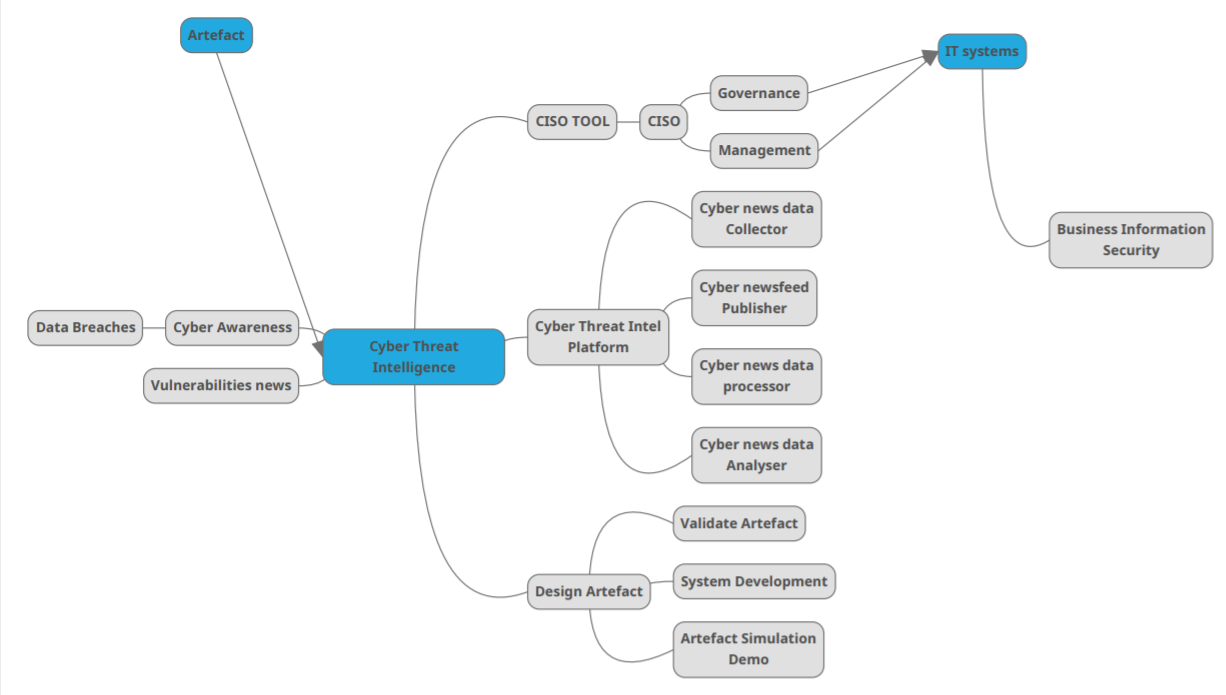
\includegraphics[width=.95\linewidth]{Figures/mindmap.png}}
    \caption{Mind Map to list Key words}
    \label{fig:info-intel}
\end{figure}
\FloatBarrier

\section{Databreaches pane picture}
\begin{figure}[ht]
    \centering
    \fbox{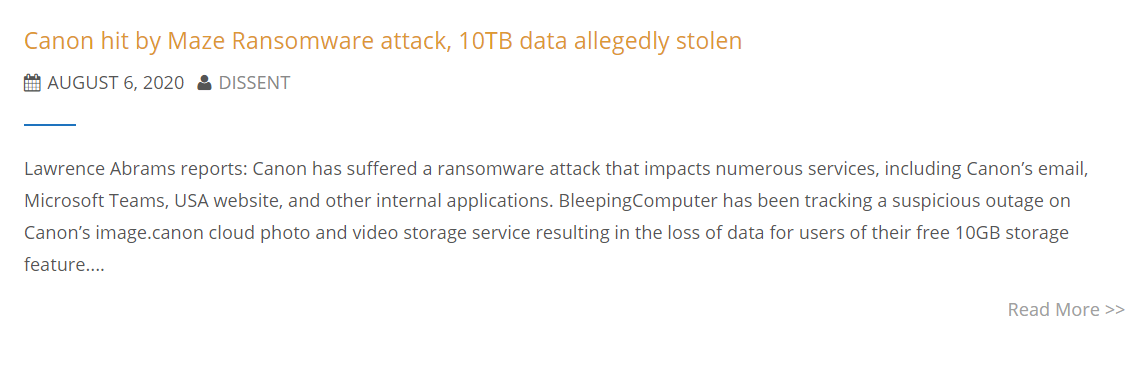
\includegraphics[width=.95\linewidth]{Figures/databreaches.PNG}}
    \caption{Databreaches pane picture}
    \label{fig:databreaches}
\end{figure}
\FloatBarrier

\section{Darkreading pane picture}
\begin{figure}[ht]
    \centering
    \fbox{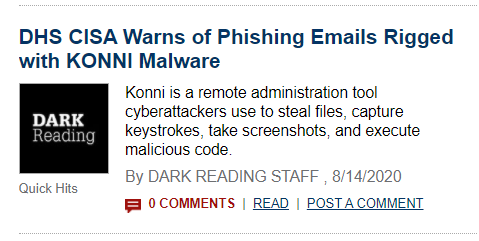
\includegraphics[width=.95\linewidth]{Figures/darkreading.PNG}}
    \caption{Darkreading pane picture}
    \label{fig:darkreading}
\end{figure}
\FloatBarrier

\chapter{Problem Domain and Research Question} % Main appendix title
\label{AppendixChapter4} 


\section{Presentation to CEO}\label{Presentation to CEO}

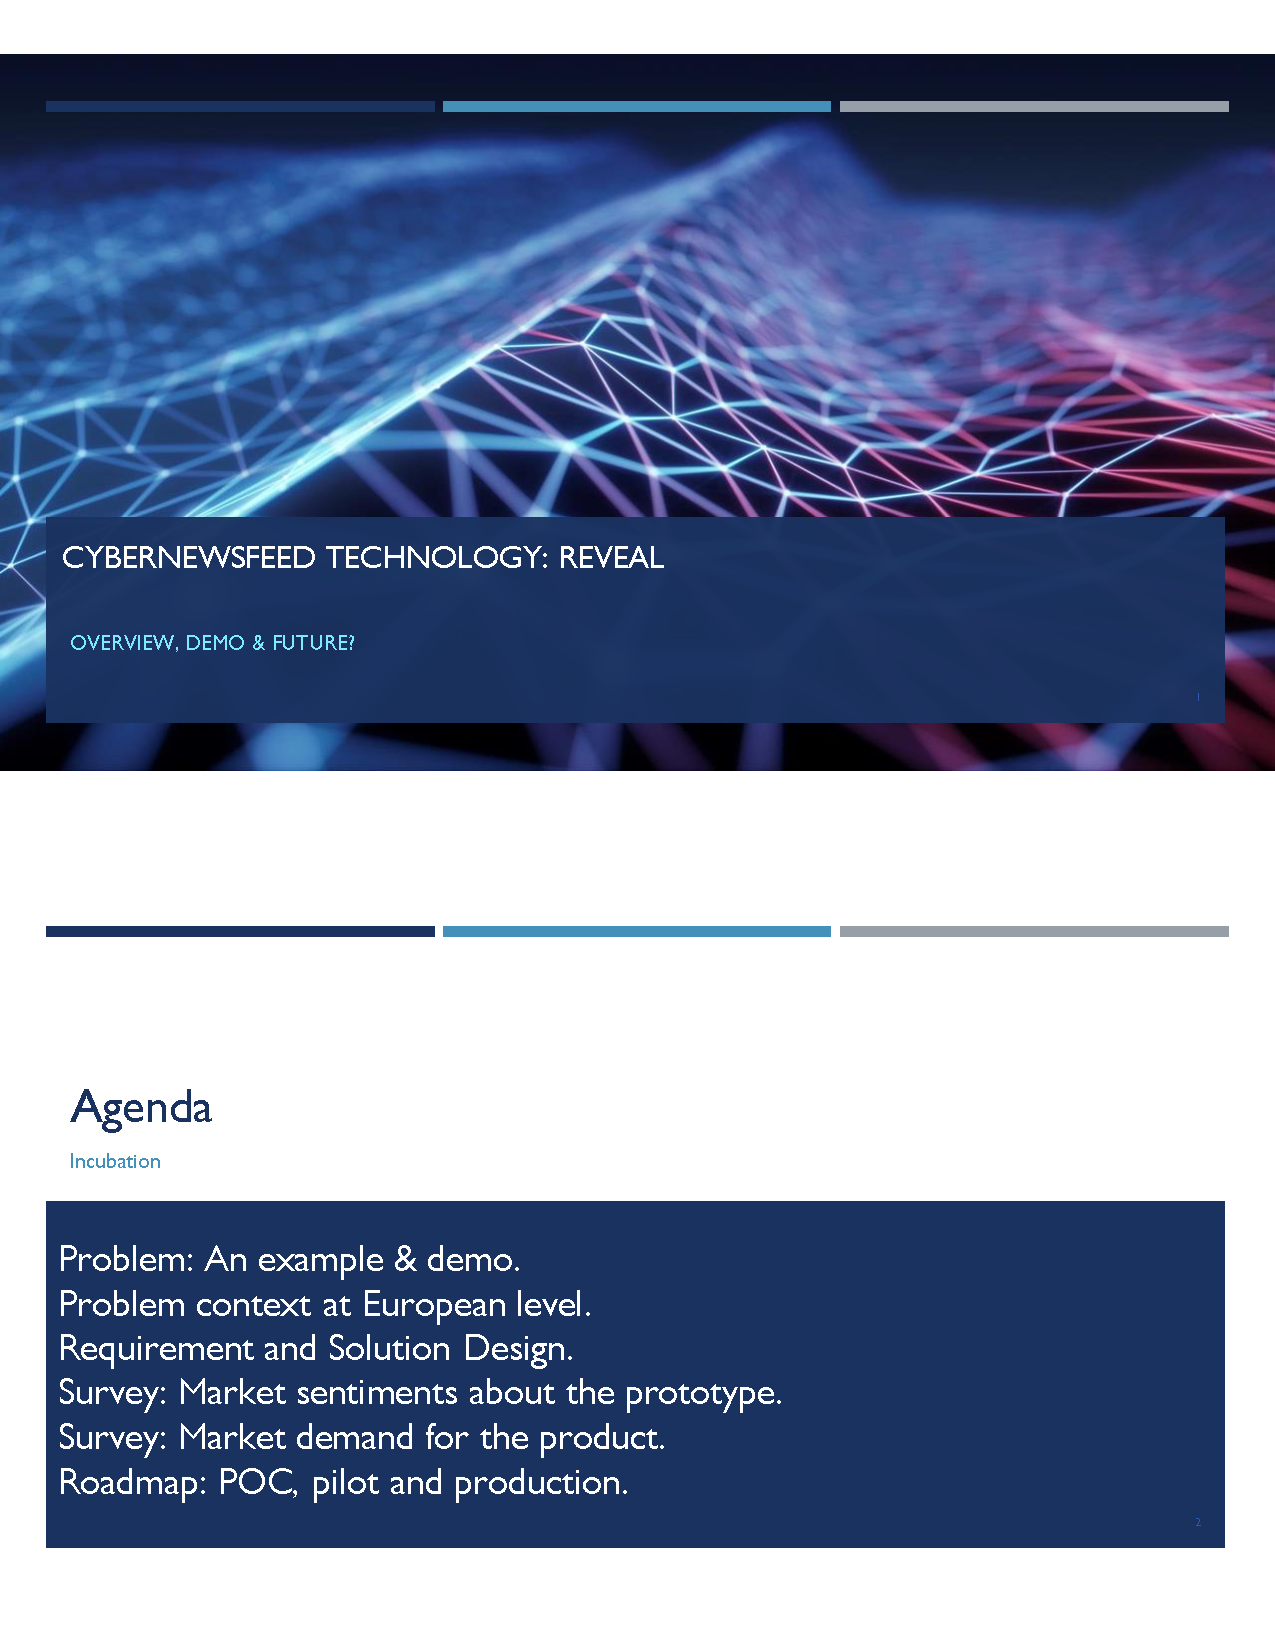
\includegraphics[page=1,scale=0.75]{Appendices/Threat-Brief-Product-marcel.pdf} 
\includegraphics[page=2,scale=0.75]{Appendices/Threat-Brief-Product-marcel.pdf} 
\includegraphics[page=3,scale=0.75]{Appendices/Threat-Brief-Product-marcel.pdf} 
\includegraphics[page=4,scale=0.75]{Appendices/Threat-Brief-Product-marcel.pdf} 

\section{Presentation to on2it}\label{Presentation to on2it}
\includegraphics[page=1,scale=0.75]{Appendices/Threat-Brief-Product-Jeroen-jean.pdf} 
\includegraphics[page=2,scale=0.75]{Appendices/Threat-Brief-Product-Jeroen-jean.pdf} 
\includegraphics[page=3,scale=0.75]{Appendices/Threat-Brief-Product-Jeroen-jean.pdf} 
\includegraphics[page=4,scale=0.75]{Appendices/Threat-Brief-Product-Jeroen-jean.pdf} 
\\includegraphics[page=5,scale=0.75]{Appendices/Threat-Brief-Product-Jeroen-jean.pdf} 
\includegraphics[page=6,scale=0.75]{Appendices/Threat-Brief-Product-Jeroen-jean.pdf} 
\includegraphics[page=7,scale=0.75]{Appendices/Threat-Brief-Product-Jeroen-jean.pdf} 
\includegraphics[page=8,scale=0.75]{Appendices/Threat-Brief-Product-Jeroen-jean.pdf} 



\section{Presentation to GSS}\label{Presentation to GSS}

\includegraphics[page=1,scale=0.75]{Appendices/GSS-Threat Brief PPT.pdf} 
\includegraphics[page=2,scale=0.75]{Appendices/GSS-Threat Brief PPT.pdf} 
\includegraphics[page=3,scale=0.75]{Appendices/GSS-Threat Brief PPT.pdf} 
\includegraphics[page=4,scale=0.75]{Appendices/GSS-Threat Brief PPT.pdf} 
%\includegraphics[page=5,scale=0.75]{Appendices/GSS-Threat Brief PPT.pdf} 

\chapter{Artefact Design} % Main appendix title

\label{AppendixChapter8} 
\label{AppendixD} % For referencing this appendix elsewhere, use \ref{AppendixA}

\section{Apply archiving to already processed data}
\begin{lstlisting}[language=SQL]
--Update Already processed data
update freshrss.on2itashishranjan_entry c set c.aging =1 
where c.aging =0 ;

--Delete old data
drop table freshrss.on2it_context ; 
--or
delete from  freshrss.on2it_context;


\end{lstlisting}
\label{tag-archiving}
\clearpage

%Importing code from file
\section{Filter to context cyber newsfeed}
\lstinputlisting[language=SQL]{Appendices/filter_context.sql}
\label{filter-context}
\clearpage

\clearpage

%Importing code from file
\section{Function to Apply TAG}
\lstinputlisting[language=SQL]{Appendices/function-sql-addtag.sql}
\label{tag-addtag}
\clearpage
%\lstinputlisting[language=Octave, caption=Octave sample code]{BitXorMatrix.m}
\section{PHP code to RSS feed}
\lstinputlisting[language=PHP]{Appendices/rss_send.php}
\label{rss-send}
\clearpage


\chapter{Artefact Evaluations } % Main appendix title

\label{AppendixChapter9} 


\section{Participants list}

\begin{table}[htbp!]
   \setlength{\arrayrulewidth}{0.5mm}
    \setlength{\tabcolsep}{5pt}
    \renewcommand{\arraystretch}{1.0}

    \centering{}
 
    \caption{Focus Group participation list}
    \label{table:expert-panel-list}
    
    \begin{tabularx}{0.92\linewidth}{|>{\columncolor[HTML]{ECB4E8}} p{3cm}|p{5.3cm}|p{3.5cm}|} 
    
%    |a|>{\columncolor[HTML]{FFFFFF}}C|C|C|
     \arrayrulecolor[HTML]{06000A}
        %% Table Body
        \hline
         \rowcolor[HTML]{BFCEED} Name & Designation & Responsibility Level \\
        \hline
     Marcel de Haan & IT Risk Manager, Montua & Stategic/Tactical \\
      \hline
Barry Derksen & Director, i-inc.nl & Strategic/Tactical \\
 \hline
Mark Butterhof & Management Consultant / Program Manager & Stategic/Tactical \\
 \hline
Pascale Van Damme & VP, EMEA VMware and Bhoomi, Dell Technology & Strategic \\
 \hline
Joshua Paffen & IT consultant & Tactical/Operational \\
 \hline
Nico J.W. Kuijper & Expert SAP Information and Privacy Governance & Stategic/Tactical \\
 \hline
Rion Rijker & Privacy Technologist, Rijker Advies  & Tactical/Operational
\\
\hline
\end{tabularx}

\end{table}






%----------------------------------------------------------------------------------------
%	BIBLIOGRAPHY
%----------------------------------------------------------------------------------------

% original call
%\printbibliography[heading=bibintoc]

% new call
\bibliography{example} 
\label{sec:bibliography}

%----------------------------------------------------------------------------------------

\end{document}  
